\author{João Gonçalves}
\newcommand{\authorr}{Teresa Nogueira}
\newcommand{\studentID}{99995}
\newcommand{\studentIDD}{100029}
%\newcommand{\supervisorone}{Prof\textsuperscript{\underline{a}}. XXXXXX}
\newcommand{\supervisorone}{}
\newcommand{\supervisortwo}{}
\newcommand{\department}{Engenharia Eletrotécnica e de Computadores}
\newcommand{\exam}{Redes de Computadores e Internet}

\title{%
Apontamentos sobre RCI\\
\large (Alguns tópicos \href{https://github.com/Kons-5}{\raisebox{0 em}{\large \faGithub}})}
\date{Fevereiro 2023}

\documentclass[a4paper,12pt]{article}
\usepackage[left=25mm,top=21mm,right=25mm,bottom=21mm]{geometry}
\usepackage[flushmargin,hang,bottom,multiple]{footmisc}
\usepackage[usestackEOL]{stackengine}
\usepackage{babel}
\usepackage[T1]{fontenc}
\usepackage[utf8]{inputenc}
\usepackage{fontawesome5,textcomp}
\usepackage{xcolor}
\usepackage{fancyhdr}

\usepackage[export]{adjustbox}
\usepackage{graphicx,array,tabularx}
\usepackage{float,wrapfig}
\usepackage[font=footnotesize]{caption}
\usepackage[justification=centering]{subcaption}

\usepackage{amsmath,amsfonts,amssymb}
\usepackage{bm}
\usepackage{mathtools}
\usepackage{mathabx}
\usepackage{physics}
\usepackage{cancel}

\usepackage{pgfplots}
\usepackage{msc}
\usepackage{booktabs}
\usepackage{tcolorbox}
\usepackage{etoolbox}

\usepackage{makecell}
\usepackage{listings}
\usepackage{enumitem}

\usepackage[linktoc=all]{hyperref}
\usepackage[capitalise]{cleveref}
\usepackage[nottoc,numbib]{tocbibind}
\usepackage[square,numbers,sort]{natbib}
\usepackage{breakurl}
\usepackage{placeins}
\usepackage{colortbl}
\usepackage{attrib}
\usepackage{multirow,multicol}

%\usepackage[printwatermark]{xwatermark}
\usepackage[framemethod=TikZ]{mdframed}
%\tcbuselibrary{skins,breakable}
%\usetikzlibrary{shadings,shadows}
\linespread{1}
%\setlength{\parindent}{0pt}

\hypersetup{
    colorlinks,
    linkcolor={black},
    citecolor={blue!50!black},
    urlcolor={blue!50!black}
}

\setlength{\abovedisplayskip}{3pt}
\setlength{\belowdisplayskip}{3pt}
\setlength{\fboxsep}{1.25\fboxsep}

\let\zzzfootnotesize\footnotesize
\def\newfootnotesize{%
\zzzfootnotesize
\abovedisplayskip=0pt
\belowdisplayskip=\abovedisplayskip
\abovedisplayshortskip=\abovedisplayskip
\belowdisplayshortskip=\abovedisplayskip
}
\renewcommand\footnotesize{\protect\newfootnotesize}

\mdfsetup{%
    linewidth=2pt
}
%//==============================--@--==============================//%
%                         -> error messages <-                        %
\usepackage{pifont}

\newenvironment{warning}
  {\par\begin{mdframed}[linewidth=1.5pt,linecolor=red]%
    \begin{list}{}{\leftmargin=0.9cm
                   \labelwidth=\leftmargin}\item[\raisebox{-0.4 em}{\Large\ding{43}}]}
  {\end{list}\end{mdframed}\par}

%//==============================--@--==============================//%
%                   -> reduzir espaço entre itens <-                  %
\usepackage{enumitem}
%\setlist[itemize]{nosep}
%\setlist[enumerate]{nosep}
\setlist[itemize]{itemsep=0.0125em}
\setlist[enumerate]{itemsep=0.0125em}
%//==============================METH-==============================//%
\newcounter{theo}[section]\setcounter{theo}{0}
\renewcommand{\thetheo}{\arabic{theo}}

%\definecolor{tempcolor}{RGB}{113, 110, 97}
\definecolor{tempcolor}{RGB}{0, 0, 0}
\newenvironment{theo}[2][]{%
    \refstepcounter{theo}
    \ifstrempty{#1}%
    % if condition (without title)
    {\mdfsetup{%
        frametitle={%
            \tikz[baseline=(current bounding box.east),outer sep=0pt]
            \node[anchor=east,rectangle,fill=blue!20]
            {\strut Teorema~\thetheo};}
        }%
    % else condition (with title)
    }{\mdfsetup{%
        frametitle={%
            \tikz[baseline=(current bounding box.east),outer sep=0pt]
            \node[anchor=east,rectangle,fill=white]
            {\strut #1};}%
        }%
    }%
    % Both conditions
    \mdfsetup{%
        innertopmargin=0pt,linecolor=tempcolor,%
        linewidth=2pt,topline=true,%
        frametitleaboveskip=1.25\dimexpr-\ht\strutbox\relax%
    }
 
\begin{mdframed}[]\relax\vspace{-0.5em}}{%
\end{mdframed}}

\def\delequal{\mathrel{\ensurestackMath{\stackon[1pt]{=}{\scriptstyle\Delta}}}}

\let\originalleft\left
\let\originalright\right
\renewcommand{\left}{\mathopen{}\mathclose\bgroup\originalleft}
\renewcommand{\right}{\aftergroup\egroup\originalright}
%------------------------------------ MAGIC--------------------------------------
\def\UrlBreaks{\do\/\do-}
\expandafter\def\expandafter\UrlBreaks\expandafter{\UrlBreaks\do\a%
\do\b\do\c\do\d\do\e\do\f\do\g\do\h\do\i\do\j\do\k\do\l\do\m\do\n%
\do\o\do\p\do\q\do\r\do\s\do\t\do\u\do\v\do\w\do\x\do\y\do\z\do\&}

\newcolumntype{C}[1]{>{\centering\let\newline\\\arraybackslash\hspace{0pt}}m{#1}}
\newcolumntype{L}[1]{>{\raggedright\let\newline\\\arraybackslash\hspace{0pt}}m{#1}}
%----------------------------------TITLE PAGE -----------------------------------
\makeatletter
\def\maketitle{
  \begin{center}\leavevmode
        \normalfont
        
\includegraphics[width=0.5\columnwidth]{img/title-page/IST.pdf}
        \vskip 0.05cm   
        \textsc{\large \department}\\
        \vskip 0.5cm
        \rule{0.95\linewidth}{0.2 mm} %\\
        {\large \exam}\\[0.5 cm]
        {\huge \bfseries \@title \par} 
        \vspace{1em}
        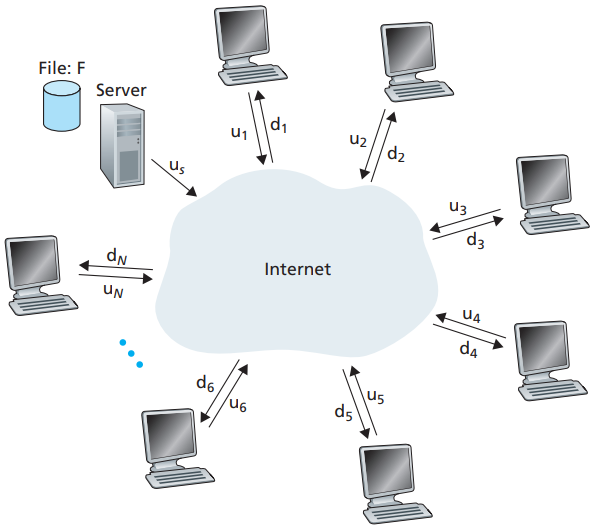
\includegraphics[scale=0.4]{img/title-page/000.png}
        \vspace{-0.5em}
        \captionof*{figure}{\color{gray} Imagem: \textit{Illustrative file distribution problem $[$Kurose \& Ross $2017]$}}
        %\vspace{0.5cm}
        \rule{0.95\linewidth}{0.2 mm} \\[0.75 cm]
        %\fontsize{9pt}{11pt}\selectfont
        \begin{minipage}[t]{1\textwidth}
	   \begin{flushleft} \large
                \emph{Autores:}\\
			\normalsize \textbf{\@author} : \studentID\\
                \fontsize{9pt}{11pt}\selectfont $\hookrightarrow$ jrazevedogoncalves@tecnico.ulisboa.pt \\
                \normalsize \textbf{\authorr} : \studentIDD\\
                \scriptsize $\hookrightarrow$ maria.teresa.ramos.nogueira@tecnico.ulisboa.pt
		\end{flushleft}
	\end{minipage}
	\vfill
        ``\textit{Let us reflect on the brief life of a bit}.''
        \vfill
	{\Large \@date\par}
   \end{center}
   %\vfill
   %\null
   \cleardoublepage
  }
\makeatother
%-------------------------------- ENDTITLE PAGE ----------------------------------
%---> Header <---
%\fancyhf{}
\renewcommand{\headrulewidth}{1pt}% Header rule width
\renewcommand{\footrulewidth}{0pt}% No footer rule
\setlength\headheight{26pt} 
\fancyhead[L]{\raisebox{0.1\height}[0pt][0pt]{\textit{Redes de Computadores e Internet}}}
\fancyhead[R]{\raisebox{0.1\height}[0pt][0pt]{2022/2023}}
%%%%%%%%%%%%%%%%%

\pgfplotsset{compat=1.18}
\setcounter{tocdepth}{3}
%\setcounter{secnumdepth}{4}
\setcounter{secnumdepth}{-2}

\renewcommand{\figurename}{Fig.}
\renewcommand{\tablename}{Tab.}
\renewcommand{\contentsname}{Índice}
\settocbibname{\raisebox{0em}{Referências}}
\setlength{\bibsep}{0.1em}%reduzir espaço entre refs.

%\renewcommand{\bibpreamble}{\vspace{-8em}}
\usepackage[titles]{tocloft}
\setlength{\cftbeforesecskip}{1em}

%\usepackage{pdfpages}
% \newwatermark[page=15,fontfamily=bch,color=red!50,angle=45,scale=3.5,xpos=-10,ypos=10]{TO BE ADDED}


\begin{document}
    \sloppy
    %% title page
    \pagenumbering{gobble}
    \maketitle
    %% toc
    \tableofcontents
    \setcounter{tocdepth}{4}
    %% body
    \newpage
    \pagestyle{fancy}
    \pagenumbering{arabic}
    
    \clearpage
    \section{1. Introdução às Redes de Computadores e à Internet}\label{sec:intro}%
        %//==============================--@--==============================//%
\subsection[1.1 Conceitos fundamentais]{\hspace*{0.075 em}\raisebox{0.2 em}{$\pmb{\drsh}$}  Conceitos fundamentais}
\label{subsec:conceitos-fundamentais}

%//==============================--@--==============================//%
\subsubsection[1.1.1 Redes de Computadores]{$\pmb{\rightarrow}$ Redes de Computadores}

Uma rede de computadores pode ser vista como um grupo de sistemas de computação conectados por meio de canais de comunicação em prole da comunicação e partilha de recursos de uma larga gama de utilizadores.

\vspace{-0.5em}
\begin{enumerate}
    \item \textbf{Sistemas terminais} (\textit{end systems or hosts})---e.g., PCs, servidores, quintas de servidores (server farms), telemóveis, laptops, frigoríficos, termostatos, etc.
    \item \textbf{Canal de comunicação} (\textit{peer-to-peer}, difusão)---abstração de comunicação cons- truida sobre um meio físico ou wireless: fios de cobre (e.g., RJ11, RJ45), cabos coaxiais (opção bastante isolada eletromagneticamente), fibra ótica (alta velocidade, opção imune a interferência eletromagnética), rádio nas suas múltiplas variantes...
    \item A interligação supramencionada é efetuada via \textbf{comutadores}, que transitam informação entre canais adjacentes.
    \item Exemplos de \textbf{serviços} de comunicação e partilha de recursos: encaminhamento de dados, garantia de entrega dos dados, autenticação, conversão entre nomes e endereços, etc.
\end{enumerate}

%//==============================--@--==============================//%
\vspace{-2em}
\subsubsection[1.1.2 Internet]{$\pmb{\rightarrow}$ Internet}

A \textit{Internet} é uma "rede de redes", global e hierarquizada, que providencia uma variedade de informação e serviços de comunicação (e.g., \textbf{aplicações distribuidas}) através da \underline{interconexão de redes} que fazem uso de \underline{protocolos} (de comunicação \textbf{standardizados}: abertos, sancionados por uma entidade competente (IETF), mas de adesão voluntária).

\begin{figure}[H]
    \centering
    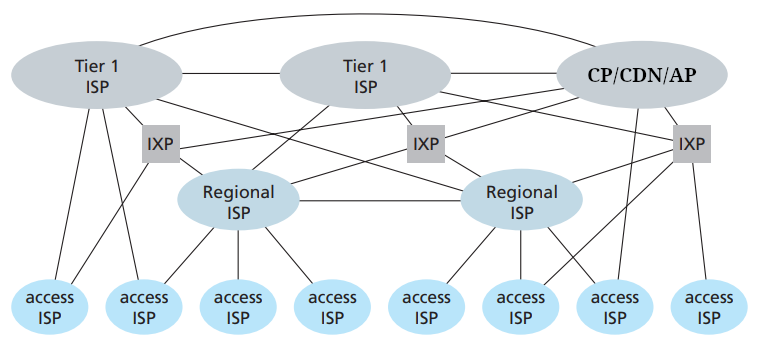
\includegraphics[width = 0.9\linewidth]{img/1/internet-ISP-interconnection.png}
    \caption{Interconexão de ISPs. ``In summary, today’s Internet--—a network of networks—--is complex, consisting of a dozen or so tier-1 ISPs and hundreds of thousands of lower-tier ISPs. The ISPs are diverse in their coverage, with some spanning multiple continents and oceans, and others limited to narrow geographic regions. The lower-tier ISPs connect to the higher-tier ISPs, and the higher-tier ISPs interconnect with one another $[$\textit{peering}, i.e., conectam as suas redes (settlement-free) de forma a que o tráfego comum passe pela conexão direta invés de por um ISP \textit{upstream}$]$.''\cite{Kurose2017}}
    \label{fig:internet}
\end{figure}

\vspace{-2em}
\begin{center}
    \scalebox{0.9}{%
    $$
        \text{CP – Content Provider} \quad \text{CDN – Content Distribution Network} \quad \text{AP – Application Provider}
    $$
    }
\end{center}

\vspace{-0.5em}
\noindent \textbf{Nota:} IXPs {\small(Internet Exchange Points)} são "pontos de encontro" para ISPs fornecidos por \textit{third-parties} que dispõem de infraestruturas independentes com os seus próprios \textbf{comutadores}.
%//==============================--@--==============================//%
\clearpage
\paragraph[1.1.2.1 Protocolos]{$\pmb{\star}$ Protocolos}\mbox{}\\[4pt]
Consideremos agora outra \textit{buzzword} importante em Redes de Computadores: \textit{protocolo}.

\vspace{-2.25em}
\begin{figure}[H] 
    \begin{subfigure}[b]{0.5\linewidth}
        \centering
        \resizebox{\columnwidth}{!}{
            \drawframe{no}
            \setmsckeyword{} %removes msc keyword from the title
            \begin{msc}[
                  normal values,
                  /msc/level height=0.6cm,
                  /msc/label distance=0.5ex,
                  /msc/first level height=0.6cm,
                  /msc/last level height=0.6cm
                ]{}
                \setlength{\instwidth}{2\mscunit} 
                \setlength{\instdist}{2\mscunit} %message width
                
                \declinst{prover}{}{\textbf{Human 1}}
                \declinst{verifier}{}{\textbf{Human 2}}
                \mess{Hi!}{prover}{verifier}
                \nextlevel[2]
                \mess{Hi!}{verifier}{prover}
                \nextlevel[2]
                \mess{Got time?}{prover}{verifier}
                \nextlevel[2]
                \mess{2:00 PM}{verifier}{prover}
            \end{msc}
        }
        \caption{Protocolo "humano".}
        \label{subfig:protocol-example1}
    \end{subfigure}%% 
    \begin{subfigure}[b]{0.5\linewidth}
        \centering
        \resizebox{\columnwidth}{!}{
            \drawframe{no}
            \setmsckeyword{} %removes msc keyword from the title
            \begin{msc}[
                  normal values,
                  /msc/level height=0.6cm,
                  /msc/label distance=0.5ex,
                  /msc/first level height=0.6cm,
                  /msc/last level height=0.6cm
                ]{}
                \setlength{\instwidth}{2\mscunit} 
                \setlength{\instdist}{2\mscunit} %message width
                
                \declinst{prover}{}{\textbf{Client}}
                \declinst{verifier}{}{\textbf{Server}}
                \mess{\footnotesize TCP connection request}{prover}{verifier}
                \nextlevel[2]
                \mess{\footnotesize TCP connection reply}{verifier}{prover}
                \nextlevel[2]
                \mess{\texttt{GET} $\left< \texttt{URL} \right>$}{prover}{verifier}
                \nextlevel[2]
                \mess{$\left< \texttt{file} \right>$}{verifier}{prover}
            \end{msc}
        }
        \caption{Protocolo de rede de computador\protect\footnotemark[1].}
        \label{subfig:protocol-example2}
    \end{subfigure}%% 
    \label{fig:exemplos-protocolos}
    \caption{Exemplos genéricos de protocolos.}
\end{figure}

\vspace{-1em}
\begin{theo}[\underline{Protocolo}]{def:protocolo}\label{def:protocolo}
    ``A \textbf{protocol} defines the format and the order of messages exchanged between two or more communicating entities, as well as the actions taken on the transmission and/or receipt of a message or other event.''\cite{Kurose2017}
\end{theo}

\noindent \textbf{Nota (no contexto computacional):} ``A \textit{protocol} is an agreement about the packets exchanged by communicating programs and what they mean. A protocol tells how packets are structured---for example, where the destination information is located in the packet and how big it is---as well as how the information is to be interpreted.''\cite{Donahoo-Kenneth2002}

\footnotetext[1]{%
    São exemplos de protocolos: TCP, UDP, HTTP/HTTPS; que veremos mais adiante.
}
%//==============================--@--==============================//%
\subsubsection[1.1.3 Breve História das Redes de Computadores e da Internet]{$\pmb{\rightarrow}$ Breve História das Redes de Computadores e da Internet}

\begin{enumerate}[noitemsep, nolistsep] \small
    \item[\textbf{1940:}] Máquina de Turing, primeira noção de um dispositivo computacional com comunicação.
    
    \item[\textbf{1960:}] Mainframes começam a ser utilizadas em universidades e instituições militares para partilhar recursos e comunicar entre si.
    
    \item[\textbf{1969:}] ARPANET, primeira rede de computadores, desenvolvida pelo Departamento de Defesa dos Estados Unidos com o objetivo de conectar instituições de pesquisa.

    \item[\textbf{1972:}] Ray Tomlinson cria o primeiro programa de correio eletrónico, expandindo as funcionalidades da ARPANET além da simples troca de arquivos.
    
    \item[\textbf{1974:}] Vint Cerf e Robert Kahn apresentam o protocolo TCP (Transmission Control Protocol), base para a comunicação na Internet.
    
    \item[\textbf{1983:}] A ARPANET adota o protocolo TCP/IP, sedimentando as bases para a Internet moderna e interconexão global de redes.
        
    \item[\textbf{1989:}] Tim Berners-Lee, no CERN, propõe a World Wide Web, um sistema global de documentos interligados por hiperligações e acessíveis pela Internet.
    
    \item[\textbf{1990:}] ARPANET é oficialmente desativada, dando lugar à Internet atual.
    
    \item[\textbf{1993:}] Mosaic, primeiro navegador gráfico da WWW, desenvolvido por Marc Andreessen e Eric Bina, populariza a Internet e atrai um público mais amplo.
    
    \item[\textbf{1994:}] O protocolo HTTP é desenvolvido por Tim Berners-Lee, facilitando a troca de informações na World Wide Web.
\end{enumerate}

\hfil \textbf{\vdots}

%//==============================--@--==============================//%
        %//==============================--@--==============================//%
\clearpage
\subsection[1.2 Multiplexagem e comutação]{\hspace*{0.075 em}\raisebox{0.2 em}{$\pmb{\drsh}$} Multiplexagem e comutação}
\label{subsec:multiplexagem-e-comutação}


\subsubsection[1.2.1 Circuit Switching]{$\pmb{\rightarrow}$ Circuit Switching}

\begin{theo}[\underline{Circuit Switching}]{def:CircuitSwitching}\label{def:CircuitSwitching}

    ``In circuit-switched networks, \textbf{the resources needed along a path} to provide for communication between the end systems \textbf{are \textit{reserved}} for the duration of the communication session between the end systems.''\cite{Kurose2017}
\end{theo}

\begin{figure}[H]
    \centering
    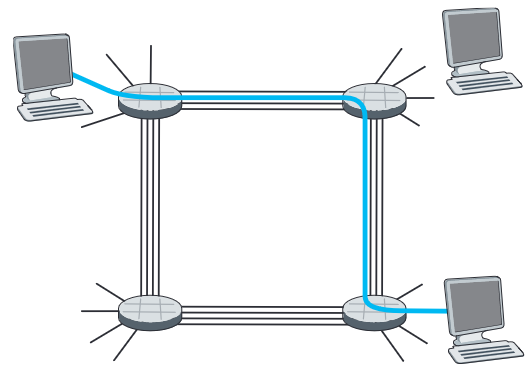
\includegraphics[width = 0.7\linewidth]{img/1/circuit-switching.png}
    \caption{Circuit Switching: ``In this network, the four circuit switches are interconnected by four links. Each of these links has four circuits, so that each link can support four simultaneous connections. The hosts (for example, PCs and workstations) are each directly connected to one of the switches. \textbf{When two hosts want to communicate, the network establishes a dedicated end-to-end connection between the two hosts.} Thus, in order for Host A to communicate with Host B, the network must first reserve one circuit on each of two links. \textbf{In this example, the dedicated end-to-end connection uses the second circuit in the first link and the fourth circuit in the second link.}''\cite{Kurose2017}}
    \label{fig:circuitswitching}
\end{figure}
\noindent A coordenação entre canal-subcanal de entrada e saída (referente à última frase da legenda da \hyperref[fig:circuitswitching]{Fig. 3}) é realizada através do uso de \textbf{tabelas de expedição} dinâmicas, que veremos mais adiante. 

\vspace{1 em}
\noindent Recorrendo novamente à \hyperref[fig:circuitswitching]{Fig. 3}, cada canal possui quatro circuitos, a velocidade trans- missão será um quarto da capacidade total do canal:

\begin{quote}
    ``Because each link has four circuits, for each link used by the end-to-end connection, the connection gets one fourth of the link’s total transmission capacity for the duration of the connection.''\cite{Kurose2017}
\end{quote}
$$
   \boxed{R_{\text{trans}} = \dfrac{R_{\text{link}}}{N}\; [\text{bps}]}
$$
\noindent Onde $N$ é o número de circuitos por canal (\textit{circuits} por \textit{link}).

%//==============================--@--==============================//%
\clearpage
\paragraph[1.2.1.1 Multiplexagem FDM]{$\pmb{\star}$ Multiplexagem FDM (\textit{frequency-division multiplexing})}\mbox{}

\begin{theo}[\underline{FDM}]{def:FDM}\label{def:FDM}
    ``With FDM, \textbf{the link dedicates a frequency band to each connection} for the duration of the connection''\cite{Kurose2017}
\end{theo}

\vspace{-0.75em}
\begin{figure}[H]
    \centering
    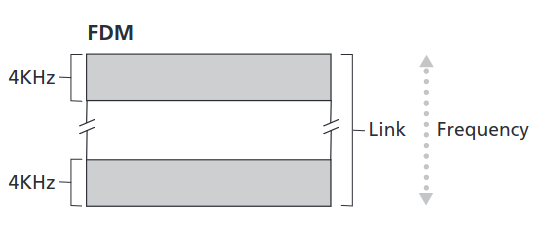
\includegraphics[width = 0.7\linewidth]{img/1/FDM.png}
    \caption{Vizualição das partições da banda de transmissão na multiplexagem de frequência}
    \label{fig:FDM}
\end{figure}

%//==============================--@--==============================//%
\paragraph[1.2.1.2 Multiplexagem TDM]{$\pmb{\star}$ Multiplexagem TDM (\textit{Time-division multiplexing})}\mbox{}

\begin{theo}[\underline{TDM}]{def:TDM}\label{def:TDM}
    ``For a TDM link, time is divided into frames of fixed duration, and each frame is divided into a fixed number of time slots. When the network establishes a connection across a link, the network dedicates one time slot in every frame to this connection.''\cite{Kurose2017}
\end{theo}

\begin{figure}[H]
    \centering
    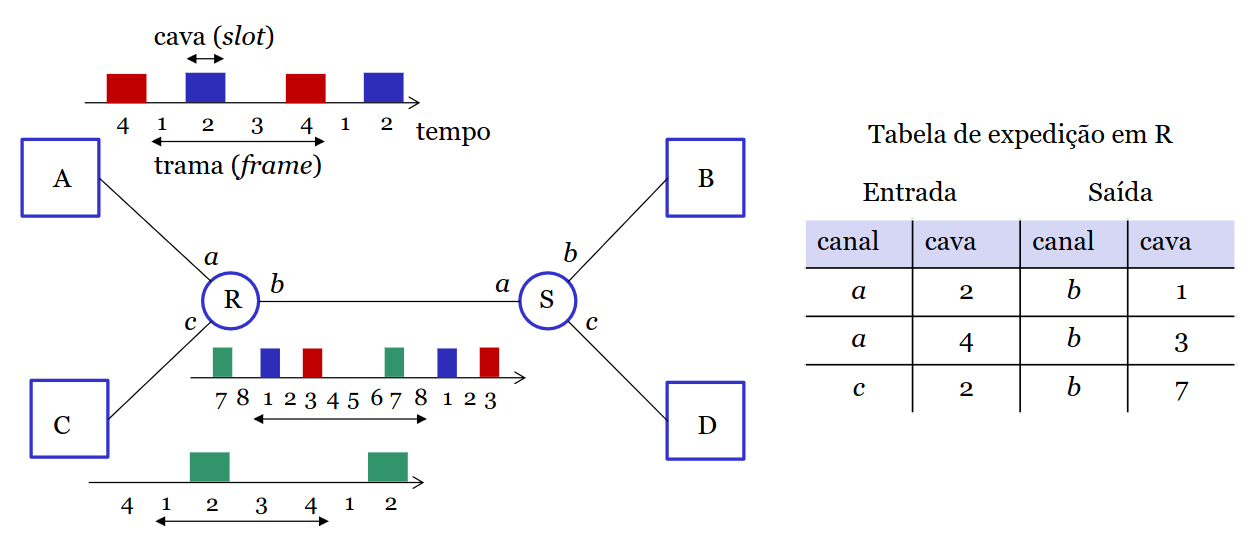
\includegraphics[width = 1\linewidth]{img/1/TDM.png}
    \caption{Time Division Mulplexing com respetiva tabela de expedição.}
    \label{fig:TDM}
\end{figure}

\noindent A informação é dividida no tempo em \textit{slots} (cavas), o conjunto de \textit{slots} origina uma estrutura denominada \textit{frame} (trama) de natureza períodica. A comutação entre canais é realizada através de tabelas de expedição que estabelecem associações entre canal e subcanal de entrada e saída:
\begin{enumerate}[label=$\rightarrow$]
    \item Na \hyperref[fig:TDM]{Fig. 5}, a informação a \textit{verde} comuta do canal $c$ para o $b$, sofrendo também uma comutação do subcanal 2 para o 7 (\textit{vide} tabela de expedição e a numerização dos slots). O mesmo processo verifica-se para a informação que comuta do canal $a$ para o canal $b$.
\end{enumerate}


%//==============================--@--==============================//%
\paragraph[1.2.1.3 Multiplexagem Determinística]{$\pmb{\star}$ Multiplexagem Determinística}\mbox{}\\[4pt]
O processo de \textit{circuit switching} é um método multiplexagem determinística (transmissão constante, certa, ``When the network establishes the circuit, it also reserves a constant transmission rate in the network’s links''\cite{Kurose2017})

{
\mdfsetup{linewidth=2pt}

\begin{mdframed}
\begin{enumerate}[label=$\blacktriangle$]
    \item Multiplexagem
        
        \vspace{-0.75em}
        \begin{itemize}
            \item Divisão de um canal em sub-canais de capacidades fixas (\textbf{TDM}, \textbf{FDM}, WDM, CDM).
        \end{itemize}
    \item Comutação (\textit{switching})
        
        \vspace{-0.75em}
        \begin{itemize}
            \item Circuito: concatenação de sub-canais ao longo de um caminho.
            \item Tabelas de expedição (fowarding table): associação entre pares de entrada (canal, sub-canal) e pares de saída (canal, sub-canal).
        \end{itemize}
        \item Circuitos dinâmicos:
        
        \vspace{-0.75em}
        \begin{itemize}
            \item Estabelecimento do circuito: atribuições de sub-canais em cada canal de um
                caminho e preenchimento das tabelas de expedição.
            \item Terminação do circuito: remoção das atribuições e limpeza das tabelas.
            \item Bloqueio se um canal não tiver um sub-canal disponível.
        \end{itemize}
\end{enumerate}
\end{mdframed}
}

%//==============================--@--==============================//%
\subsubsection[1.2.2 Packet Switching]{$\pmb{\rightarrow}$ Packet Switching}

\begin{theo}[\underline{Packet Switching}]{def:PacketSwitching}\label{def:PacketSwitching}

    ``\textbf{The source breaks long messages into smaller chunks of data known as \textit{packets}}. Between source and destination each packet travels through communication
    links and \textbf{\textit{packet switches}}---a router takes a packet arriving on one of its attached communication links and forwards that packet onto another one of its attached communication
links''\cite{Kurose2017}
\end{theo}

\renewcommand*{\thefootnote}{\fnsymbol{footnote}}
\footnotetext[1]{%
    ``Finally, there are two different ways to pronounce the word router, either as “rootor” or as “rowter,” and people waste a lot of time arguing over the proper pronunciation [Perlman 1999].''\cite{Kurose2017}
}
\renewcommand*{\thefootnote}{\arabic{footnote}}

\vspace{-1em}
\begin{figure}[H]
    \centering
    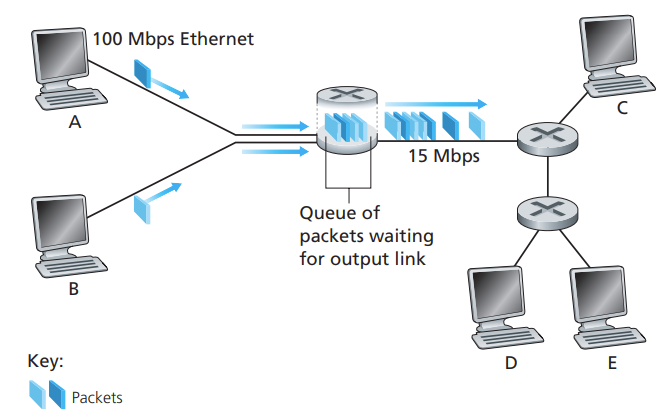
\includegraphics[width = 0.8\linewidth]{img/1/packet-switching.png}
    \caption{Packet Switching}
    \label{fig:PacketSwitching}
\end{figure}

\noindent Estes pacotes viajam com um ritmo igual ao ritmo total de transmissão do canal. Neste sentido, supondo o envio de um pacote de dimensão $L$ bits por um canal com capacidade $R$ bits/sec, o intervalo de tempo de transmissão é dado por:
$$
   \boxed{d_{\text{trans}} = \dfrac{L}{R}\; [\text{s}]}
$$
%//==============================--@--==============================//%
\paragraph[1.2.2.1 Store and Forward Transmission]{$\pmb{\star}$ Store and Forward Transmission}\mbox{}

\begin{theo}[\underline{Store and Forward Transmission}]{def:Store-For-Trans}\label{def:Store-For-Trans}
    ``Store-and-forward transmission means that \textbf{the packet switch \textit{must} receive the entire packet} before it can begin to transmit the first bit of the packet onto the outbound link.''\cite{Kurose2017}
\end{theo}
Pressupondo a transmissão de um pacote até um \textit{router} (\textit{packet switcher}) que aplica \textit{Store and Forward Transmission}, a subsequente comutação e transmissão para outro canal é apenas executada quando o \textit{router} possuir o pacote completo. Assim os bits já recebidos do pacote sofrem \textit{buffering} (são armazenados em fila de espera) até o \textit{router} possuir o pacote integral e proceder à sua transmissão.

\vspace{-1.2em}
\begin{figure}[H]
    \centering
    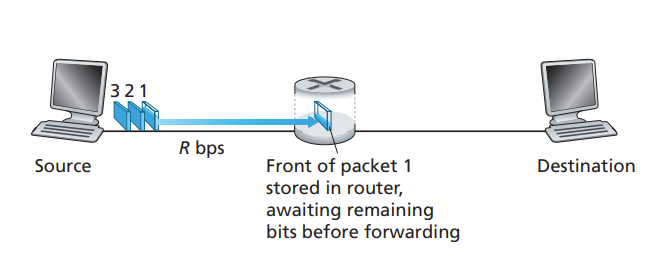
\includegraphics[width = 0.8\linewidth]{img/1/store-and-forward.png}
    \caption{Store and Forward transmission}
    \label{fig:Store-For}
\end{figure}

\noindent O tempo de espera resultante do processo de \textit{buffering} denomina-se de \textbf{\textit{queuing delay}}, $d_{\text{queue}}$. Este \textit{delay} é aleatório e está dependente do nível de \textbf{congestionamento} do canal (a taxa de chegada de pacotes a um comutador é superior à sua capacidade). Por outro lado o espaço da linha de espera é finito. Num caso extremo de congestionamento a linha de espera poderá encontrar-se totalmente preenchida, pacotes acabados de chegar poderão ser parcialmente ou totalmente perdidos, ocorre \textit{\textbf{packet loss}}.

%//==============================--@--==============================//%
\paragraph[1.2.2.2 Forwarding Tables and Routing Protocols]{$\pmb{\star}$ Forwarding Tables and Routing Protocols}\mbox{}

\begin{theo}[\underline{Forwarding Tables}]{def:Ftables}\label{def:Ftables}
    ``(...) Each router has a forwarding table that maps destination addresses (or portions of the destination addresses) to that router’s outbound links. \textbf{When a packet arrives at a router, the router examines the address and searches its \textit{forwarding table}}, using this destination address, \textbf{to find the appropriate outbound link}.''\cite{Kurose2017}
\end{theo}
\clearpage
As tabelas de expedição (\textit{forwarding tables}, localizadas nos cabeçalhos dos pacotes) são elaboradas automaticamente com recurso a \textit{\textbf{routing protocols}}:

\begin{quote}
    ``A \textbf{\textit{routing protocol}} may, for example, determine the shortest path from each router to each destination and use the shortest path results to configure the forwarding tables in the routers.''\cite{Kurose2017}
\end{quote}

%//==============================--@--==============================//%
\paragraph[1.2.2.3 Multiplexagem Estatística]{$\pmb{\star}$ Multiplexagem Estatística}\mbox{}\\[4pt]
\noindent O processo de \textit{packet switching} é um método de multiplexagem estatística---decorre da partilha assíncrona de um canal entre pacotes e obedece à política \textit{first come first served} (a transmissão de pacotes é realizada por ordem de chegada). A qualidade estatística refere-se ao caráter aleatória do congestionamento e \textit{rate} de transmissão:

{
\mdfsetup{linewidth=2pt}

\begin{mdframed}
    \begin{enumerate}[label=$\blacktriangle$]
        \item Multiplexagem
    
            \vspace{-0.75em}
            \begin{itemize}
                \item Mensagens e \textit{data streams} são divididas em pacotes (\textit{packages}) de pequena dimensão.
                \item Partilha assíncrona (no tempo) de um canal entre pacotes.
                \item Cabeçalhos distinguem os pacotes.
                \item Os cabeçalhos (\textit{headers}) dos pacotes contêm informação que permite o seu
                posterior reagrupamento nos dados originais.
            \end{itemize}
        \item Comutação
    
            \vspace{-0.75em}
            \begin{itemize}
                \item \textit{Store-and-forward}: cada mensagem é recebida na
                totalidade antes de ser expedida.
                \item As tabelas de expedição estabelecem a localização do subsequente \textit{outbound-link} através da associação entre terminais de entrada e saída.
            \end{itemize}
        \item \textbf{Equidade} na partilha dos recursos de transmissão e comutação (\textit{switching}).
        \item \textbf{Congestionamento} se a taxa de chegada de mensagens a um comutador for
    superior à capacidade deste, conduzindo a atrasos e, possivel perdas.
    \end{enumerate}%adoro-te :3
\end{mdframed}
}

\noindent \textbf{Nota:} Ao não executar a partição de dados em pacotes de menor tamanho a transmissão fica sujeita a períodos de \textbf{inequidade} (\textit{starvation}): quando uma mensagem longa impede o despacho de
mensagens curtas.

%//==============================--@--==============================//%
\subsubsection[1.2.3 Circuit Switching vs. Packet Switching]{$\pmb{\rightarrow}$ Circuit Switching vs. Packet Switching}
\vspace{-1 em}
\begin{table}[H]
    \begin{tabularx}{\linewidth}{>{\parskip1ex}X@{\kern4\tabcolsep}>{\parskip1ex}X}
    \toprule
    \hfil\bfseries Circuit Switching
    &
    \hfil\bfseries Packet Switching
    \\\cmidrule(r{3\tabcolsep}){1-1}\cmidrule(l{-\tabcolsep}){2-2}
    
    %% separated by empty line or \par
    Ideal para aplicações que exigem comu- nicação confiável/determinística, como as redes telefónicas.\par
    Fornece uma qualidade de serviço consis- tente.\par
    Requer um caminho dedicado durante toda a sessão de comunicação, mesmo durante períodos de inatividade.
    &
    
    %% separated by empty line or \par
    Garante flexibilidade e eficiência para redes com um elevado número de uti- lizadores.\par
    Experiência de comunicação imprevisível, graças à política de \textit{first come first served}.\par
    Mais simples, mais eficiente (em termos de recursos), e menos dispendiosa de implementar
    \\\bottomrule
    \end{tabularx}
    \caption{Pros \& cons dos tipos de comutação abordados.}
\end{table}
%//==============================--@--==============================//%
\subsubsection[1.2.4 Virtual Circuits]{$\pmb{\rightarrow}$ Virtual Circuits}

\begin{theo}[\underline{Virtual Circuits}]{def:virtual-circuits}\label{def:virtual-circuits}
    ``Virtual circuits provide a logical, \textbf{pre-determined path within a packet-switched network}, such as Frame Relay, Asynchronous Transfer Mode (ATM), and Multiprotocol Label Switching (MPLS) networks. Virtual circuits use statistical multiplexing, which is an intrinsic feature of packet-switched networks, allowing multiple virtual circuits to share the same physical links and resources, leading to better utilization of network resources and increased efficiency.'' $[$\textbf{?}$]$
\end{theo}

\vspace{-1em}
\begin{figure}[H]
    \centering
    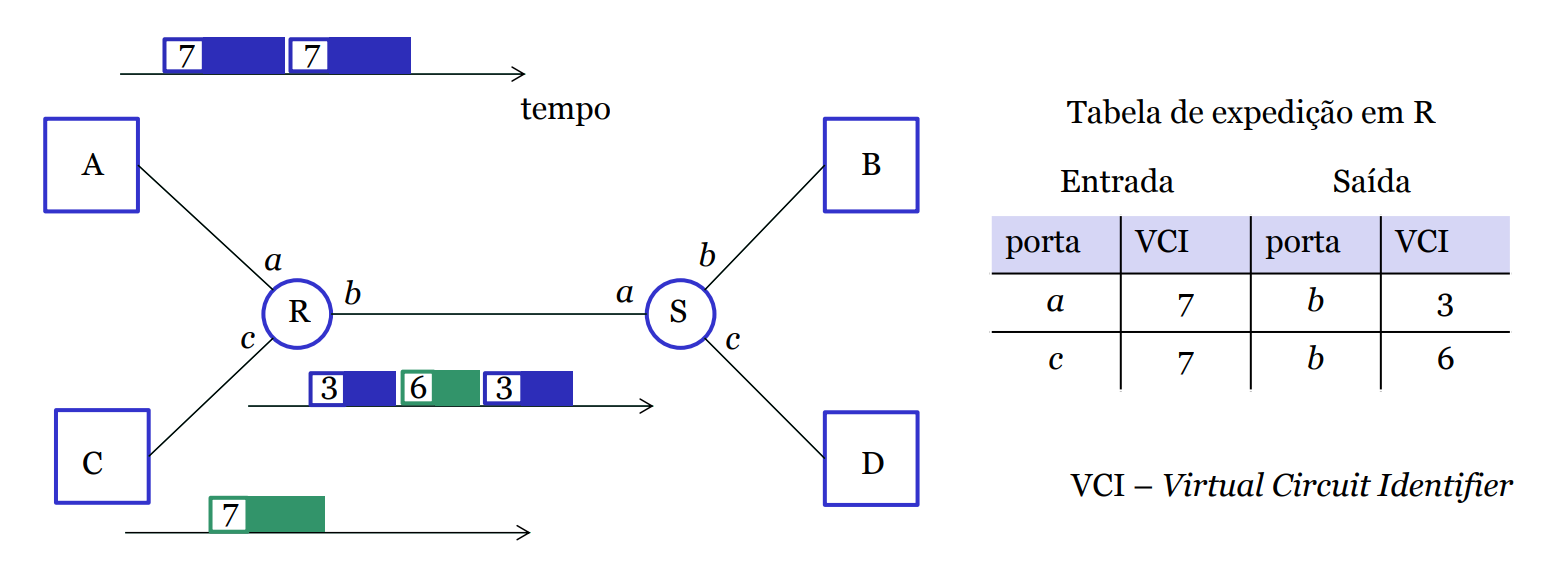
\includegraphics[width = 0.9\linewidth]{img/1/virtual-circuits.png}
    \caption{Circuitos virtuais.\protect\cite{slidesSobrinho}}
    \label{fig:virtual-circuits}
\end{figure}

\noindent While virtual circuits do not reserve a fixed bandwidth like traditional circuit-switched networks, they can offer certain advantages such as:
\begin{itemize}[label=$\blacktriangle$]
    \item \textbf{Established path}, which may lead to more consistent performance compared to purely connectionless packet switching.
    \item \textbf{In-order delivery} of packets, as they follow the same pre-determined path.
\end{itemize}

\noindent By allowing multiple virtual circuits to share the same physical links and resources, virtual circuits provide greater flexibility and efficiency compared to traditional circuit-switched networks.
        \input{src/1/débitos-e-atraso}
        \clearpage
%//==============================--@--==============================//%
\subsection[1.4 Arquitetura em camadas]{\hspace*{0.075 em}\raisebox{0.2 em}{$\pmb{\drsh}$} Arquitetura em camadas}
\label{subsec:arquitetura-em-camadas}

De modo a que a rede (de protocolos) tome uma estrutura, é necessário organizar os \textbf{protocolos} (tomamos uma abordagem em camadas---em que cada protocolo pertence a uma camada). Refletimos sobre os \textbf{serviços} que uma camada providencia à camada diretamente acima (\textbf{service-model} da camada).

\begin{quote}
    ``(...) each layer provides its service by (1) performing certain actions within that layer and by (2) using the services of the layer directly below it.''\cite{Kurose2017}
\end{quote}

\noindent Uma camada pode ser implementada em \textit{software}, em \textit{hardware}, ou numa combinação de ambos; e é usual que os componentes integrantes da rede (e.g., sistemas terminais, comutadores, etc.) tenham partes do protocolo da camada $n$ \textit{distribuídos} entre si.

Este modelo (\textit{protocol layering}) apresenta vantagens estruturais\footnotemark[2] e conceptuais que nos permitem chegar à \textit{pilha de protocolos da Internet}:

\vspace{-0.5em}
\begin{figure}[H]
    \centering
    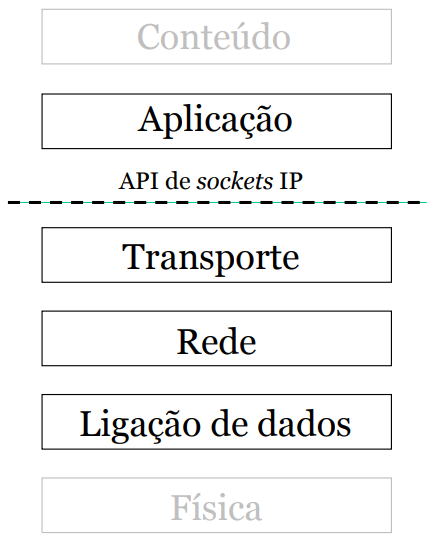
\includegraphics[width = 0.3\linewidth]{img/1/pilha-de-protocolos.png}
    \raisebox{7.5em}{
        \begin{minipage}{0.65\linewidth}
            \begin{enumerate}[label=$\bullet$]\small
                \item \textbf{Camada de Aplicação} -- Protocolos dependentes da aplicação em causa (HTTP/HTTPS, SMTP, ...)
                \item \textbf{Camada de Transporte} -- Controlo de erros e de fluxo extremo-a-extremo, controlo de congestionamento  (transferência de dados entre processos; TCP, UDP, etc.)

                \vspace{-0.75em}
                \hfill {\footnotesize \textit{transport-layer packets $\rightarrow$ \textbf{segments}}}
                \item \textbf{Camada de Rede}\footnotemark[3] -- Encaminhamento e expedição global (dos \textit{datagramas})

                \vspace{-0.75em}
                \hfill {\footnotesize \textit{network-layer packets $\rightarrow$ \textbf{datagrams}}}
                \item \textbf{Camada de Ligação} -- Controlo de erros local, en- caminhamento e expedição local, controlo de acesso ao meio (Ethernet, Wi-Fi, PPP, ...) \hfill {\footnotesize \textit{link-layer $\rightarrow$ \textbf{frames}}}
            \end{enumerate}
        \end{minipage}
    }
    \caption{Modelo simplificado da Internet---pilha de protocolos.}
    \label{fig:pilha-de-protocolos-internet}
\end{figure}

\phantomsection\addcontentsline{toc}{subsubsection}{1.4.1 Encapsulamento de dados}

\vspace{-1.5em}
\begin{figure}[H]
    \centering
    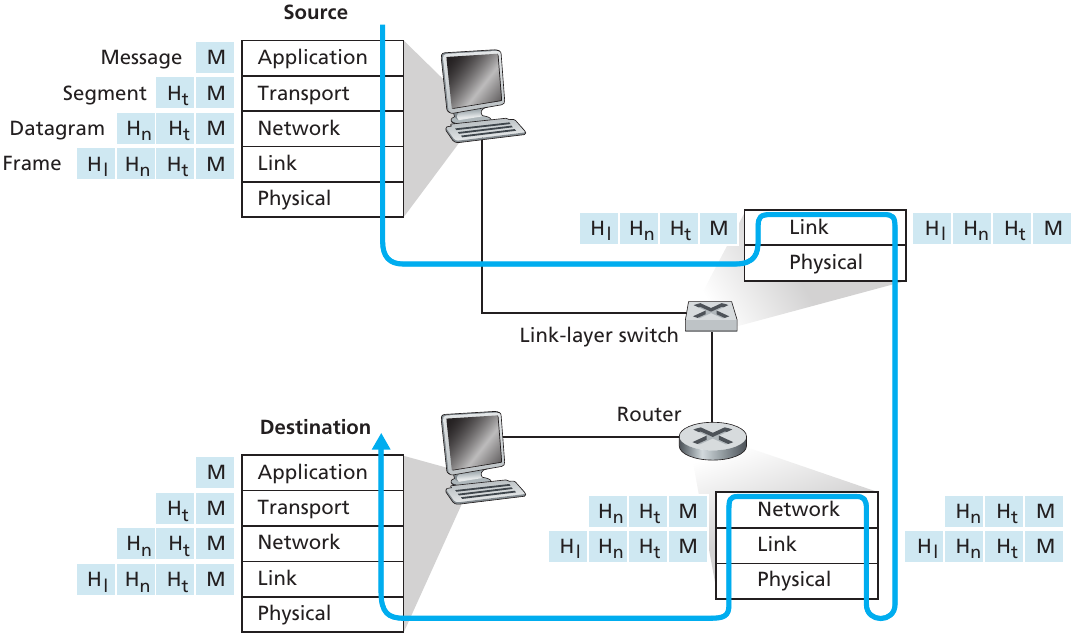
\includegraphics[width = 0.65\linewidth]{img/1/encapsulation.png}
    \hfill \raisebox{8.25em}{
        \begin{minipage}{0.3\linewidth}
            \parbox{\textwidth}{%
                \small \texttt{Identificadores na \textquotesingle net}: nomes e endereços p/ \textit{layer}.
            }

            \vskip 0.35em
            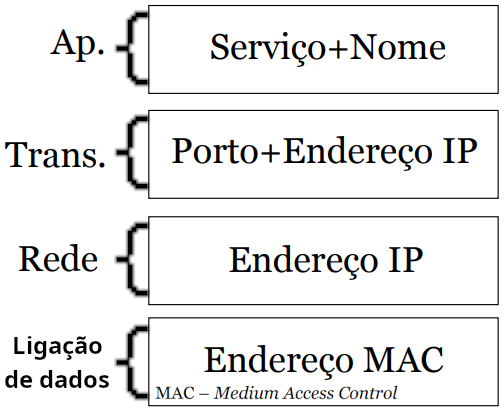
\includegraphics[width = 1\linewidth]{img/1/identifiers.png}
        \end{minipage}
    }
    \caption{Cada componente da rede dispõe de um conjunto de camadas, o que reflete a diferença entre as suas funcionalidades. \textbf{Encapsulamento:} o pacote da camada $N$ é constituído pelo cabeçalho da camada $N$ mais o pacote da camada $N + 1$.}
    \label{fig:encapsulation}
\end{figure}

\footnotetext[2]{%
    ``For large and complex systems that are constantly being updated, the ability to change the implementation of a service without affecting other components of the system $[$veja-se como modularidade$]$ is another important advantage of layering.''\cite{Kurose2017}
}
\footnotetext[3]{%
    ``Although the network layer contains both the IP protocol and numerous routing protocols, it is often simply referred to as the IP layer, reflecting the fact that IP is the glue that binds the Internet together.''\cite{Kurose2017}
}

\renewcommand*{\thefootnote}{\fnsymbol{footnote}}
\footnotetext[4]{%
    \textbf{Nota:}\hfill API -- Application Programming Interface \qquad\quad IP -- Internet Protocol.
}
\renewcommand*{\thefootnote}{\arabic{footnote}}
%//==============================--@--==============================//%

    \clearpage
    \section{2. Camada de Aplicação}\label{sec:application-layer}%
        %//==============================--@--==============================//%
\subsection[2.1 Arquiteturas de aplicação de redes]{\hspace*{0.075 em}\raisebox{0.2 em}{$\pmb{\drsh}$}  Arquiteturas de aplicação de redes}
\label{subsec:arquitetura-aplicacao-redes}

\begin{theo}[\underline{Application Architecture}]{def:AppArch}\label{def:AppArch}
    ``The application architecture, on the other hand, is designed by the application developer and dictates how the application is structured over the various end systems. In choosing the application architecture, an application developer will likely draw on one of the two predominant architectural paradigms used in modern network applications: \textbf{the client-server architecture} or the \textbf{peer-to-peer (P2P)} architecture.''\cite{Kurose2017}
\end{theo}

%//==============================--@--==============================//%
\subsubsection[2.1.1 Client-server architecture]{$\pmb{\rightarrow}$ \textit{Client-server architecture}}

Em arquiteturas cliente-servidor (\textit{client-server architectures}) um servidor (\textit{always-on host}) \textbf{providência os seus serviços a múltiplos clientes}: ``A classic example is the Web application for which an always-on Web server services requests from browsers running on client hosts." onde \textbf{os clientes não comunicam diretamente entre si} (o servidor é responsável pela manutenção e comunicação entre clientes). Os servidores \textbf{possuem um IP fixo}, garantindo um fluxo de comunicação constante. Para garantir o processamento de um elevado tráfego de pedidos são utilizados \textit{data centers} que albergam múltiplos \textit{hosts}:

\begin{quote}
    ``The most popular Internet services—such as search engines (e.g., Google, Bing, Baidu), Internet commerce (e.g., Amazon, eBay, Alibaba), Web-based e-mail (e.g., Gmail and Yahoo Mail), social networking (e.g., Facebook, Instagram, Twitter, and WeChat)—employ one or more data centers."\cite{Kurose2017}
\end{quote}

%//==============================--@--==============================//%
\subsubsection[2.1.2 Peer-to-Peer (P2P)]{$\pmb{\rightarrow}$ \textit{Peer-to-Peer (P2P)}}

Em arquiteturas \textit{peer-to-peer} (P2P) a comunicação é independente de servidores. A aplicação procura estabelecer contacto direto entre pares de \textit{hosts} ligados intermitentemente designador por \textit{peers}. Estes \textit{host} residem nas máquinas dos utilizadores (e.g. casa, universidades, escritorios, ...). A comunicação P2P é dotada de \textit{self-scalability}:

\begin{quote}
    ``For example, in a P2P file-sharing application, although each peer generates workload by requesting files, each peer also adds service capacity to the system by distributing files to other peers."\cite{Kurose2017}
\end{quote}

\vspace{-0.5 em}
\begin{table}[H]
    \begin{tabularx}{\linewidth}{>{\parskip1ex}X@{\kern4\tabcolsep}>{\parskip1ex}X}
    \toprule
    \hfil\bfseries Client-server architecture
    &
    \hfil\bfseries Peer-to-Peer (P2P) 
    \\\cmidrule(r{3\tabcolsep}){1-1}\cmidrule(l{-\tabcolsep}){2-2}
    
    %% separated by empty line or \par
    O servidor é dependente de \textit{data centers} que necessitam de manutenção e energia.\par
    Pagamento de \textit{recurring interconnection and bandwidth costs} na transmissão de dados.\par
    Seguro e estável, face à arquitetura \textit{peer-to-peer}
    &
    
    %% separated by empty line or \par
    \textit{Cost efficient}, não dependente de infraestruturas de larga escala.\par
    ``Face challenges of security, performance, and reliability due to their highly
    decentralized structure."\par
    \textit{Self-scalability}.
    \\\bottomrule
    \end{tabularx}
    \caption{Pros \& cons dos tipos de arquitetura de aplicação abordados.}
\end{table}
%//==============================--@--==============================//%
\subsubsection[2.1.3 Comunicação entre processos ]{$\pmb{\rightarrow}$ Comunicação entre processos}

\begin{theo}[\underline{Processo (Process)}]{def:Processo}\label{def:Processo}
    ``In the jargon of operating systems, it is not actually programs but processes that
communicate. \textbf{A process can be thought of as a program that is running within an end
system}. When processes are running on the same end system, they can communicate
with each other with \textbf{interprocess communication}. Processes on two different end systems communicate with each other by \textbf{exchanging messages across the computer network}.''\cite{Kurose2017}
\end{theo}

\noindent Uma aplicação de rede consiste na troca de mensagens entre pares de processos. Cada par possui um processo designado cliente e outro servidor, mediante a tarefa desempenhada no início da sessão de comunicação:

\begin{quote}
    ``In the context of a communication session between a pair of processes, \textbf{the process that initiates the communication} (that is, initially contacts the other process at the beginning of the session) \textbf{is labeled as the client. The process that waits to be contacted to begin the session is the server}."
\end{quote}

\noindent Um processo envia e recebe mensagens da rede através de uma interface designada \textit{socket} que estabelece a ligação entre a camada de aplicação e a camada de transporte da qual o programador pouco controlo tem com exceção da escolha do protocolo em uso. Este tema será explorado na \hyperref[subsec:socket-programming]{secção 2.x}.

%//==============================--@--==============================//%
\subsubsection[2.1.4 Endereçamento de processos ]{$\pmb{\rightarrow}$ Endereçamento de processos}

A identificação do processo de destino numa sessão de comunicação está dependente de dois identificadores:

\paragraph[2.1.4.1 Endereço IP]{$\pmb{\star}$ Endereço IP:} Identifica o \textit{host} na internet.

\begin{mdframed}
    ``Internet addresses are binary numbers. They come in two flavors, corresponding to the two versions of the Internet Protocol that have been standardized. The most common is version 4 (IPv4); the other is version 6 (IPv6), which is just beginning to be deployed. IPv4 addresses are 32 bits long; because this is only enough to identify about 4 billion distinct destinations, they are not really big enough for today’s Internet. For that reason, IPv6 was introduced. IPv6 addresses are 128 bits long.''\cite{Donahoo-Kenneth2002}
    
    \vspace{1 em}
    \noindent \textbf{Exemplo:} IPv4 – 193.136.128.169 \hspace*{0.75em} IPv6 – 2001:690:21c0:a::150
\end{mdframed}

\paragraph[2.1.4.2 Porto]{$\pmb{\star}$ Porto:} Especifica o processo de chegada (a socket de chegada) dentro do \textit{host}, já que este poderá estar a correr várias aplicações em simultâneo.

\begin{mdframed}
    ``Port numbers are the same in both IPv4 and IPv6: 16-bit unsigned binary numbers. Thus, each one is in the range 1 to 65,535 (0 is reserved)''\cite{Donahoo-Kenneth2002}
\end{mdframed}

%//==============================--@--==============================//%
\subsubsection[2.1.5 Serviços fornecidos pela camada de transporte ]{$\pmb{\rightarrow}$ Serviços fornecidos pela camada de transporte}
\begin{tabular}{|c|p{11cm}|}
\hline
\textbf{Category} & \textbf{Description} \\
\hline
\multirow{2}{*}{Reliable Data Transfer} & A transport-layer protocol guarantees that data sent by one end is correctly and completely delivered to the other end. \\
\hline
\multirow{4}{*}{Throughput} & A transport-layer protocol can provide a guaranteed available throughput at a specified rate, appealing to bandwidth-sensitive applications. Elastic applications can use any available throughput. \\
\hline
\multirow{3}{*}{Timing} & A transport-layer protocol can provide timing guarantees, ensuring data delivery within a specified time frame. This is essential for interactive real-time applications. \\
\hline
\multirow{3}{*}{Security} & A transport protocol can provide security services such as encryption, data integrity, and end-point authentication to protect data transmitted between processes. \\
\hline
\end{tabular}

\begin{figure}[H]
    \centering
    \includegraphics[width = 0.95\linewidth]{img/2/serviços-camada-transporte.png}
    \caption{Requisitos de algumas aplicações de redes.\cite{Kurose2017}}
    \label{fig:serviços-camada-transporte}
\end{figure}

\paragraph[2.1.5.1 Transmission Control Protocol (TCP)]{$\pmb{\star}$ Transmission Control Protocol (TCP)}\mbox{}\\[4pt]
\noindent O protocolo TCP fornece um serviço orientado à sessão (connection-oriented) de transferência fiável (\textit{reliable data transfer}) e entrega sequencial de pacotes. Serviços orientados à sessão envolvem um processo de \textit{handshaking} entre cliente e servidor de modo a trocar informação de controlo e preparar ambos os lados para a transmissão de dados, esta transmissão é bidirecional. Possui um mecanismo de \textit{congestion control} e \textbf{não fornece garantias de atraso nem de débito}.

\paragraph[2.1.5.2 User Datagram Protocol (UDP)]{$\pmb{\star}$ User Datagram Protocol (UDP)}\mbox{}\\[4pt]
\noindent UDP é um protocolo de transporte \textit{lightweight} que providência serviços minimos e não envolve processo de \textit{handshaking} (é \textit{connectionless}) \textbf{não possui uma transferência fiável nem garante uma entrega sequencial de pacotes}.

        \clearpage
%//==============================--@--==============================//%
\subsection[2.2 The Web \& HTTP]{\hspace*{0.075 em}\raisebox{0.2 em}{$\pmb{\drsh}$} The Web \& HTTP}
\label{subsec:the-web-and-http}

\begin{theo}[\underline{World Wide Web (WWW)}]{def:WWW}\label{def:WWW}
    ``The WWW is a global information space that consists of interconnected documents (Web pages) and resources accessible through the internet. The Web is built on top of the \hyperref[def:HTTP]{Hypertext Transfer Protocol (HTTP)}, which is a fundamental protocol used for transmitting and sharing data between web browsers (clients) and web servers.''
\end{theo}

%//==============================--@--==============================//%
\subsubsection[2.2.1 HTTP overview]{$\pmb{\rightarrow}$ HTTP overview}

\begin{theo}[\underline{Hypertext Transfer Protocol (HTTP)}]{def:HTTP}\label{def:HTTP}
    ``HTTP is an application-layer protocol that enables the exchange of documents, images, videos, and other resources on the World Wide Web. It uses a client-server model, where the client initiates requests and the server responds with the requested resource or an error message.''

    \vspace{-0.75em}
    \begin{enumerate}
        \item \textbf{Request-Response Cycle}: Clients (usually web browsers) send HTTP requests to servers, which respond with the requested resource or an error message.
        \item \textbf{HTTP Methods}: HTTP defines several methods, such as \texttt{GET}, \texttt{POST}, \texttt{PUT}, \texttt{DELETE}, and others, to specify the desired action to be performed on the requested resource.
        \item \textbf{HTTP Status Codes}: Servers respond with HTTP status codes to indicate the outcome of an HTTP request. Common status codes include 200 (OK), 404 (Not Found), and 500 (Internal Server Error).
    \end{enumerate}

    \noindent $\pmb{\rightarrow}$ \textbf{Nota:} HTTP utiliza \textbf{TCP} como protocolo de transporte!
\end{theo}

\noindent HTTP é dito um \textit{stateless protocol}, dado que um servidor HTTP n\~ao retem informaç\~ao acerca do utilizador:

\begin{quote}
    ``If a particular client asks for the same object twice in a period of a few seconds, the server does not respond by saying that it just served the object to the client; instead, the server resends the object, as it has completely forgotten what it did earlier.''\cite{Kurose2017}
\end{quote}

\noindent ``HTTP has evolved through several versions, each introducing new features and improvements:
\begin{itemize}
    \item \textbf{HTTP/1.0:} The initial version of HTTP, supporting basic request-response communication and using non-persistent connections.
    \item \textbf{HTTP/1.1:} An updated version that introduced persistent connections, chunked encoding, and improved caching mechanisms.
    \item \textbf{HTTP/2:} A more recent version that offers significant performance improvements, such as multiplexing, header compression, and server push.
    \item \textbf{HTTP/3:} The latest version, currently under development, which aims to improve performance further by using the QUIC transport protocol instead of TCP.'' $[$\textbf{?}$]$
\end{itemize}

%//==============================--@--==============================//%
\subsubsection[2.2.2 Persistência]{$\pmb{\rightarrow}$ Persistência}

\begin{theo}[\underline{Persistência}]{def:Persist}\label{def:Persist}
    ``(...) The application developer needs to make an important decision—should each request/response pair be sent over a separate TCP connection, or should all of the requests and their corresponding responses be sent over the same TCP connection? In the former approach, the application is said to use non-persistent connections; and in the latter approach, persistent connections.''
\end{theo}

\paragraph[2.2.2.1 Sessão não persistente]{$\pmb{\star}$ Sessão não persistente}\mbox{}

\begin{figure}[H]
    \centering
    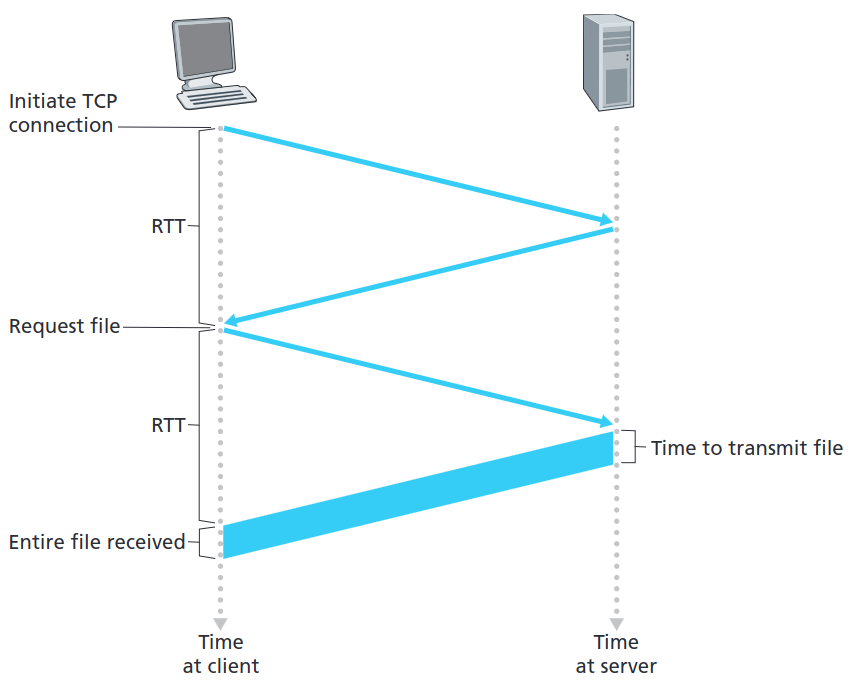
\includegraphics[width = 0.85\linewidth]{img/2/nao-resistente.png}
    \caption{Sessão TCP não persistente}
    \label{fig:nao-persistente}
\end{figure}

\noindent Suponhamos o começo de uma sessão TCP entre um \textit{browser} e um \textit{Web server}. É inicializado o procedimento \textit{three-way handshake}: O cliente (\textit{browser}) envia um pequeno segmento TCP ao servidor, subsequentemente o servidor recebe-o com sucesso e envia de volta um outro segmento TCP. Após completar as primeiras duas partes do \textit{handshake} o cliente envia um pedido HTTP incluindo também a terceira parte do \textit{handshake} (o reconhecimento da receção do segundo segmento). A conexão é solidificada, falta agora atender ao pedido:

\begin{enumerate}
    \item O servidor HTTP busca o objeto de pesquisa, encapsula-o numa mensagem de resposta HTTP e envia-a para o cliente através da \textit{socket}.
    \item O processo servidor indica o termínio da sessão TCP (embora esta não feche até saber o cliente recebeu a mensagem de forma intact).
    \item O cliente recebe a mensagem e consequentemente a sessão TCP é terminada.
\end{enumerate}

\noindent O tempo total de resposta é:
$$
    \boxed{\text{RTT} + \text{RTT} + \text{Time to transmit file}}
$$
\noindent Onde RTT (\textit{round-trip time}) é o tempo que um segmento TCP demora a viajar do cliente ao servidor e viceversa. ``The RTT includes packet-propagation delays, packet-queuing delays in intermediate routers and switches, and packet-processing delays."\cite{Kurose2017}

\vspace{0.6 em}
\noindent\textbf{Nota:} As sessões TCP não persistentes podem decorrer em paralelo, ``most browsers open 5 to 10 parallel TCP connections, and each of these connections handles one request-
response transaction (\textit{forking})"

\paragraph[2.2.2.2 Sessão persistente]{$\pmb{\star}$ Sessão persistente}\mbox{}\\[4pt]
\noindent Na sessões TCP persistentes ocorrem múltiplas transações HTTP por sessão TCP e o servidor não fecha a sessão TCP depois de responder a um pedido. Ocorre canalização (\textit{pipelining}) de pedidos, as respostas são enviadas na ordem de receção:

\vspace{1 em}
\begin{mdframed}
    ``Non-persistent connections in HTTP have limitations, such as the need to establish a new connection for each requested object and a two RTT delivery delay for each object. HTTP 1.1 introduced persistent connections, which allow the server to keep the TCP connection open for multiple requests and responses between the client and server. This enables sending an entire web page or multiple pages from the same server over a single persistent TCP connection. \textbf{Requests can be made back-to-back (pipelining) without waiting for replies to pending requests, and the server typically closes the connection after a configurable timeout interval of inactivity}."
\end{mdframed}

\begin{figure}[H]
    \centering
    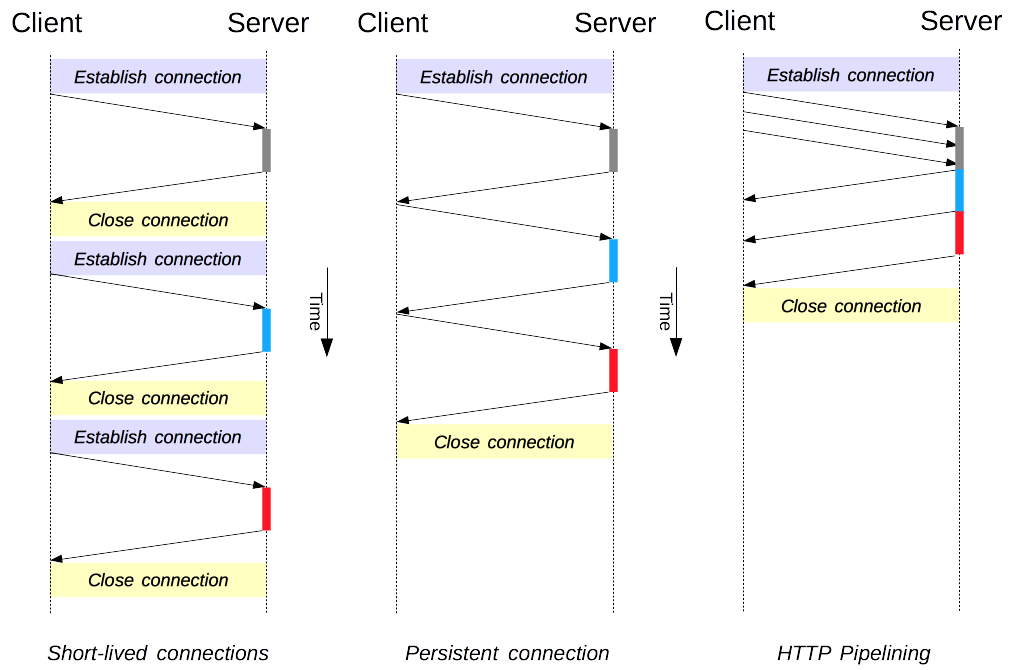
\includegraphics[width = 0.9\linewidth]{img/2/http-connections-example.png}
    \caption{Connection management in HTTP.}
    \label{fig:http-connection-example}
\end{figure}

%//==============================--@--==============================//%
\clearpage
\subsubsection[2.2.3 Transfer-Encoding: chunked]{$\pmb{\rightarrow}$ Transfer-Encoding: chunked}

Chunked encoding is a method used in HTTP to transmit data in smaller, manageable pieces (\textit{chunks}) instead of sending the entire resource in one go.

\vspace{-0.5em}
\begin{enumerate}
    \item \textbf{Purpose:} Enable the server to start transmitting data without knowing the total size of the resource, which is useful for dynamic content generation or when the resource size is unknown in advance.
    \item \textbf{Chunks:} Data is divided into separate chunks, each with its own \underline{size} specified \underline{at the beginning}. The \underline{size is followed by the actual data} and a newline character.
    \item \textbf{Transmission:} The server sends each chunk one by one, with the client assembling the received chunks to reconstruct the original resource.
    \item \textbf{End of data:} A special chunk with a size of zero signals the end of the data transmission, allowing the client to know when it has received the entire resource.
    \item \textbf{Benefits:} Improved responsiveness, as the client can start processing data as soon as the first chunk is received, and reduced resource usage, as the server doesn't need to buffer the entire resource before sending.
\end{enumerate}

\vspace{-0.75em}
\begin{figure}[H]
    \centering
    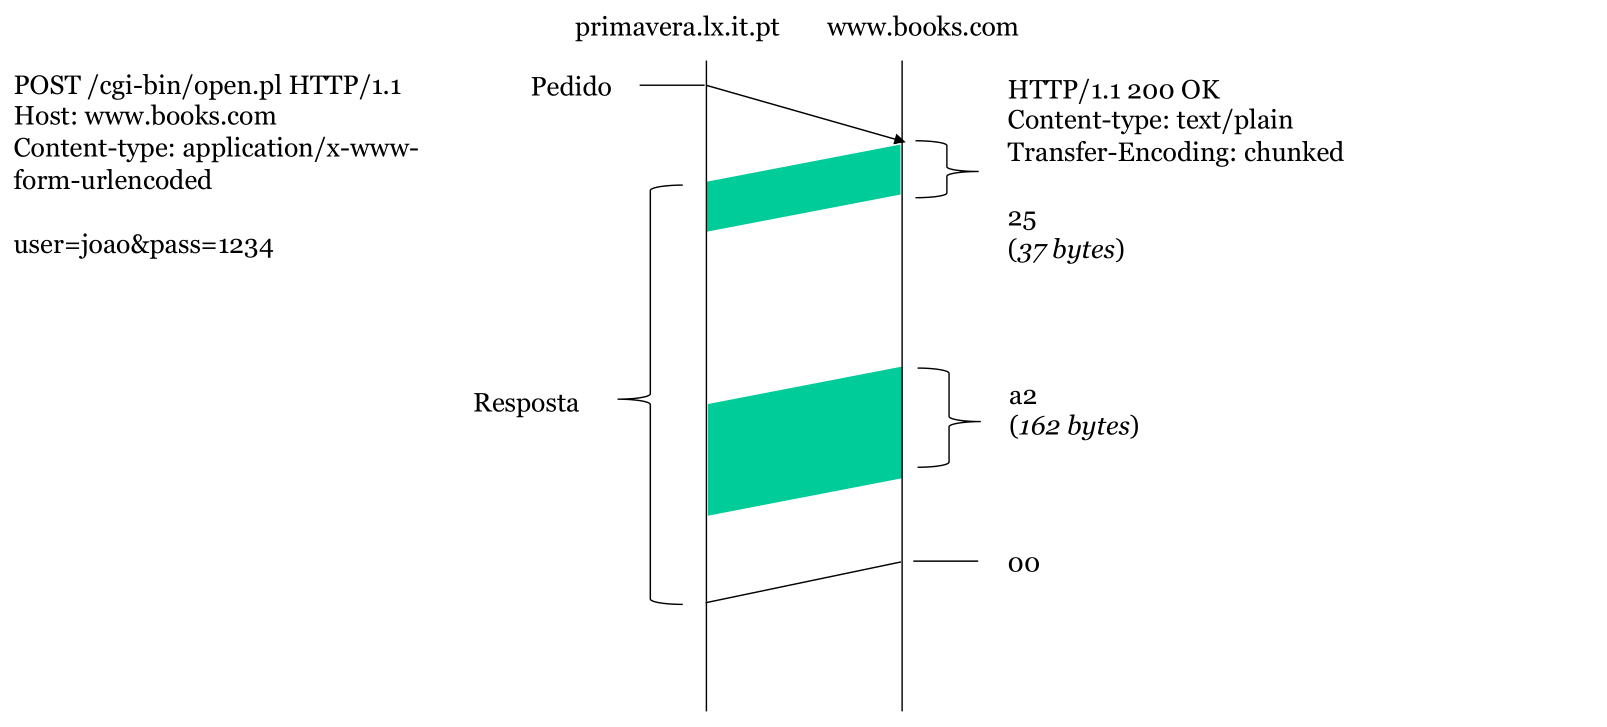
\includegraphics[width = 0.9\linewidth]{img/2/chunked-encoding.png}
    \caption{``Transfer-Encoding: chunked''\protect\cite{slidesSobrinho}}
    \label{fig:chunked-encoding}
\end{figure}

%//==============================--@--==============================//%
\subsubsection[2.2.4 Redirection]{$\pmb{\rightarrow}$ Redirection}

Redirection is a mechanism used in HTTP to inform a client that a requested resource is available at a different URL and instruct it to retrieve the resource from that new location.

\vspace{-0.5em}
\begin{enumerate}
    \item \textbf{Purpose}: Enable web servers to move or rename resources, load balance requests across multiple servers, or enforce URL canonicalization for SEO purposes.
    \item \textbf{HTTP status codes}: Redirection is signaled using HTTP status codes in the 3xx range, with each code indicating a specific type of redirection (e.g., 301 Moved Permanently, 302 Found, 303 See Other, 307 Temporary Redirect).
    \item \textbf{Location header}: The server provides the new URL for the resource in the Location HTTP header of the response. The client should follow the new URL to access the requested resource.
    \item \textbf{Considerations}: Excessive or circular redirections can lead to poor user experience and increased server load. It is essential to use the appropriate status codes and manage redirects properly to avoid such issues.
\end{enumerate}

%//==============================--@--==============================//%
\clearpage
\subsubsection[2.2.5 Formato de mensagens HTTP]{$\pmb{\rightarrow}$ Formato de mensagens HTTP}

HTTP communication relies on a request-response model, where the client initiates a request, and the server sends back a response. This exchange typically consists of four components:
\begin{enumerate}
    \item \textbf{Request/Response Line}
    \item \textbf{Headers:} Provides metadata about the request or response, such as content type, content length, and encoding.
    \item \textbf{Blank Line:} A separator between the headers and the message body.
    \item \textbf{Message Body (optional):} Contains the data being sent in the request or response, such as an HTML document or form data.
\end{enumerate}

\paragraph[2.2.5.1 HTTP request]{$\pmb{\star}$ HTTP request}\mbox{}

\begin{figure}[H]
    \centering
    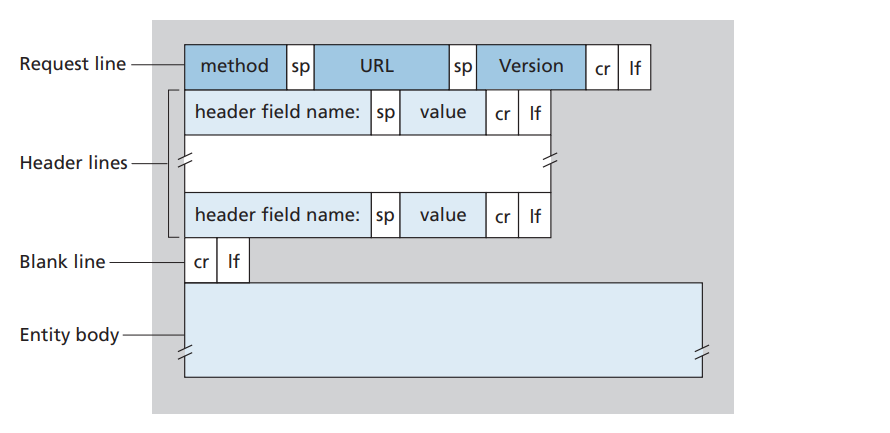
\includegraphics[width = 0.9\linewidth]{img/2/http-request-format.png}
    \caption{``General format of an HTTP request message.''\cite{Kurose2017}}
    \label{fig:http-request-format}
\end{figure}

\noindent HTTP defines several methods (also known as verbs) that indicate the action to be performed on the requested resource. Some of the most common methods include:
\begin{itemize}
    \item \texttt{GET}: Requests data from a specified resource.
    \item \texttt{POST}: Submits data to a specified resource for processing, usually resulting in a change on the server.
    \item \texttt{PUT}: Updates the specified resource with the supplied data.
    \item \texttt{DELETE}: Deletes the specified resource.
    \item \texttt{HEAD}: Similar to \texttt{GET}, but only requests the headers, without the actual data.
    \item \texttt{OPTIONS}: Retrieves the communication options available for the specified resource.
\end{itemize}

\renewcommand*{\thefootnote}{\fnsymbol{footnote}}
\footnotetext[4]{%
A \textit{Uniform Resource Locator (URL)} is a standardized address format used to locate resources on the internet. URLs typically consist of a protocol (e.g., \texttt{http}, \texttt{https}), a domain name or IP address, an optional port number, and a path to the specific resource. For example, \texttt{https://example.com:80/path/to/resource} is a URL, where \texttt{https} is the protocol, \texttt{example.com} is the domain name, \texttt{80} is the port number, and \texttt{/path/to/resource} is the path to the desired resource.
}
\renewcommand*{\thefootnote}{\arabic{footnote}}

\clearpage
\paragraph[2.2.5.2 HTTP response]{$\pmb{\star}$ HTTP response}\mbox{}

\begin{figure}[H]
    \centering
    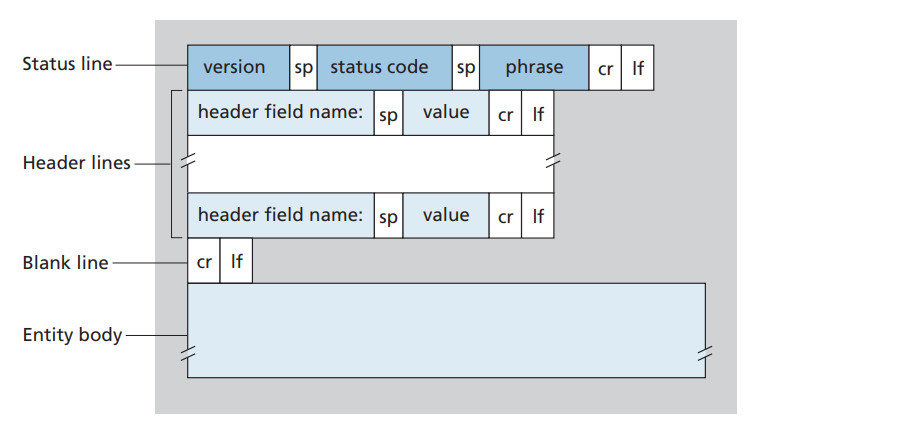
\includegraphics[width = 0.9\linewidth]{img/2/http-response-format.png}
    \caption{``General format of an HTTP response message.''\cite{Kurose2017}}
    \label{fig:http-response-format}
\end{figure}

\noindent HTTP status codes are three-digit numbers included in server responses that indicate the result of the client's request. They are categorized into five classes, based on the first digit:
\begin{itemize}
    \item \textbf{1xx (Informational):} Request received, and the server is continuing to process it.
    \item \textbf{2xx (Successful):} Request successfully received, understood, and accepted.
    \item \textbf{3xx (Redirection):} Request needs further action to be completed, such as following a different URL.
    \item \textbf{4xx (Client Error):} The request contains bad syntax or cannot be fulfilled by the server.
    \item \textbf{5xx (Server Error):} The server failed to fulfill a valid request.
\end{itemize}

%//==============================--@--==============================//%
\subsubsection[2.2.6 Interaç\~ao Cliente-Servidor: \textit{Cookies}]{$\pmb{\rightarrow}$ Interaç\~ao Cliente-Servidor: \textit{Cookies}}

Cookies are small text files stored on a user's device, allowing web applications to remember stateful information across sessions, such as preferences or login data.

\begin{enumerate}
    \item \textbf{Creation:} Servers generate cookies and send them to user's devices via \texttt{Set-Cookie} HTTP headers. The user's web browser then stores the cookie on the device.
    \item \textbf{Cookie usage:} In subsequent requests to the same website, the user's web browser automatically sends the cookie back to the server via the Cookie HTTP header. The server can then use the information in the cookie to customize the user's experience, for example, by displaying a message or remembering items in a shopping cart.
    \item \textbf{Cookie Management:} Websites can update or delete cookies; users can manage them via browser settings.
    \item \textbf{Privacy concerns:} While cookies provide a convenient way to maintain state across multiple sessions, they can also raise privacy concerns due to their ability to track users' browsing habits and collect personal information. Regulations such as the EU's General Data Protection Regulation (GDPR) aim to protect user privacy by requiring websites to obtain user consent before setting cookies and providing options for users to opt-out of tracking.
\end{enumerate}

%//==============================--@--==============================//%
\subsubsection[2.2.7 Web caching]{$\pmb{\rightarrow}$ \textit{Web caching}}

Web cachingis a technique to improve the efficiency and reduce the latency of web access by storing copies of frequently requested resources on a local cache server---also called a \textbf{proxy server}.

\begin{enumerate}
    \item \textbf{Purpose:} Reduce the load on origin servers, decrease network traffic, and improve user experience by providing faster response times.
    \item \textbf{Cache server:} A dedicated server that stores copies of resources, such as images or HTML files, to serve user requests without contacting the origin server.
    \item \textbf{Cache hit:} When a requested resource is found in the cache server, it's called a cache hit. The cache server then serves the resource directly to the user.
    \item \textbf{Cache miss:} When a requested resource is not found in the cache server, it's called a cache miss. The cache server must fetch the resource from the origin server, store it locally, and serve it to the user.
    \item \textbf{Cache replacement:} Due to limited storage capacity, cache servers employ replacement policies (e.g., Least Recently Used) to determine which resources to evict when the cache is full.
    \item \textbf{Conditional \texttt{GET}:} To ensure content freshness, cache servers can issue conditional \texttt{GET} requests, which only retrieve a resource if it has changed since the cache server's last fetch.
    \item \textbf{Collaborative caching:} Cache servers can work together to share resources, reducing redundant downloads and improving overall caching efficiency.
\end{enumerate}

\paragraph[2.2.6.1 Conditional \texttt{GET}]{$\pmb{\star}$ Conditional \texttt{GET}}\mbox{}

\begin{enumerate}
    \item \textbf{\texttt{If-Modified-Since}:} The client includes the \texttt{If-Modified-Since} HTTP header in its request, specifying the date and time of its last request for the resource. The server checks whether the resource has been modified since the specified date and time.
    \item \textbf{Resource status:} If the resource has been modified, the server sends the updated resource along with a 200 OK status code. If the resource has not been modified, the server sends a 304 Not Modified status code without the resource content, indicating that the client's cached version is still valid.
    \item \textbf{\texttt{ETag} and \texttt{If-None-Match}:} An alternative method uses the \texttt{ETag} (Entity Tag) header, which represents a unique identifier for the resource's current version. The client includes the \texttt{If-None-Match} header in its request, containing the \texttt{ETag} value received in the previous response. If the server's current \texttt{ETag} for the resource does not match the value in the \texttt{If-None-Match} header, the server sends the updated resource and its new \texttt{ETag}. If the \texttt{ETags} match, the server responds with a 304 Not Modified status code.
    \item \textbf{Cache validation:} Conditional \texttt{GET} is a crucial component of HTTP caching, as it allows clients to validate their cached resources and refresh them when necessary, without having to download the entire resource each time.
    \item \textbf{Performance benefits:} By reducing the amount of data transferred and allowing clients to reuse cached resources, conditional \texttt{GET} improves network efficiency, reduces server load, and results in faster load times for end users.
\end{enumerate}

%//==============================--@--==============================//%
\clearpage
\subsubsection[2.2.8 HTTP/2: Bloqueio topo-da-fila (\textit{head-of-line blocking})]{$\pmb{\rightarrow}$ HTTP/2: Bloqueio topo-da-fila (\textit{head-of-line blocking})} %adoro-te

\begin{theo}[\underline{Head-of-line blocking (HOL)}]{def:HOL}\label{def:HOL}
    ``Head-of-line blocking (HOL blocking) in computer networking is a performance-limiting phenomenon that occurs when a line of packets is held up in a queue by a first packet.''
\end{theo}

\noindent A versão HTTP/1.1 procura evitar este fenómeno recorrendo à abertura de várias sessões TCP paralelas, permitindo a renderização de objetos mais pequenos e subsequentemente diminuindo o \textit{user-perceived delay}. No entanto, o mecanismo de controlo de congestão inerente ao protocolo TCP força a abertura inadvertida de múltiplas conexões paralelas (exaustando assim as \textit{sockets} do sistema operativo):

\begin{quote}
     ``TCP congestion control inadvertently encourages browsers to use multiple parallel TCP connections instead of a single persistent connection. This is because congestion control aims to distribute an equal share of the available bandwidth to each TCP connection sharing a bottleneck link. By opening multiple parallel connections, a browser can "cheat" and acquire a larger portion of the link bandwidth."\cite{Kurose2017}
\end{quote}

\noindent A versão HTTP/2 procura otimizar o uso da funcionalidade de controlo de congestão bem como reduzir o número de conexões paralelas abertas:

\begin{itemize}
  \item \textbf{Framing e Multiplexagem de streams}: HTTP/2 breaks messages into small frames and interleaves request and response messages on the same TCP connection, significantly reducing user-perceived delay.
  The framing sub-layer of HTTP/2 breaks down HTTP messages into independent frames and reassembles them on the other end. This allows for interleaving and more efficient processing.
  
  \item \textbf{Binary encoding e compressão}: Frames are binary encoded (uma frame para o cabeçalho e outras múltiplas para o corpo da resposta), making them more efficient to parse, slightly smaller, and less error-prone.
  
  \item \textbf{Response message prioritization}: Clients can prioritize responses by assigning a weight between 1 and 256, allowing the server to send higher-priority frames first. Clients can also state each message's dependency on other messages.
  
  \item \textbf{Server pushing}: HTTP/2 enables servers to send multiple responses for a single client request, pushing additional objects to the client without the client having to request each one. This eliminates extra latency due to waiting for requests. (Servidor envia objetos que sabe que o cliente vai precisar sem que este lhe envie os pedidos correspondentes).
\end{itemize}

\begin{figure}[H]
    \centering
    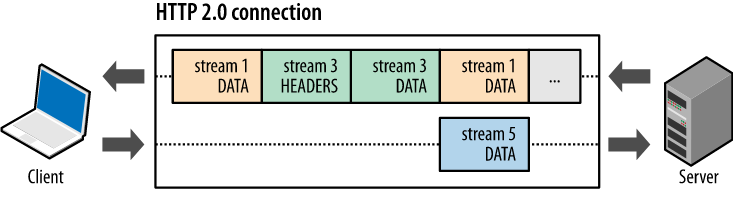
\includegraphics[width = 0.9\linewidth]{img/2/HTTP2.png}
    \caption{Multiplexagem de \textit{streams} de \textit{frames}}
    \label{fig:http2}
\end{figure}
        \clearpage
%//==============================--@--==============================//%
\subsection[2.3 Eletronic Mail (email)]{\hspace*{0.075 em}\raisebox{0.2 em}{$\pmb{\drsh}$} Eletronic Mail (email)}
\label{subsec:eletronic-mail}

%//==============================--@--==============================//%
\subsubsection[2.3.1 Simple Mail Transfer Protocol (SMTP)]{$\pmb{\rightarrow}$ Simple Mail Transfer Protocol (SMTP)}

\begin{theo}[\underline{Simple Mail Transfer Protocol (SMTP)}]{teo/def:SMTP}\label{teo/def:SMTP}
    ``SMTP is the principal application-layer protocol for Internet electronic mail. It uses the reliable data transfer service of TCP to transfer mail from the sender’s mail server to the recipient’s mail server. As with most application-layer protocols, SMTP has two sides: a client side, which executes on the sender’s mail server, and a server side, which executes on the recipient’s mail server."\cite{Kurose2017}
\end{theo}

\noindent \textbf{Nota:} ``SMTP restricts the body (not just the headers) of all mail messages to simple 7-bit ASCII'' \& ``does not normally use intermediate mail servers for sending mail, even when the two mail servers are located at opposite ends of the world.''´. Assim, se o servidor de destino estiver inativo, a receção da mensagem está dependente do reenvio por parte do servidor do utilizador, não permanecendo num servidor de resguardo temporário.

\definecolor{codegray}{rgb}{0.5,0.5,0.5}
\begin{lstlisting}[language=, title={Exemplo SMTP \protect\cite{slidesSobrinho}}, frame=tb, basicstyle=\footnotesize\ttfamily\color{codegray}]
S: 220 destino.pt
C: HELO origem.pt
S: 250 Hello origem.pt, pleased to meet you
C: MAIL FROM: fernando@origem.pt
S: 250 fernando@origem.pt ... Sender ok
C: RCPT TO: luis@destino.pt
S: 250 luis@destino.pt ... Recipient ok
C: DATA
S: 354 Enter mail, end with "." on a line by itself
C: From: fernando@origem.pt
C: To: luis@destino.pt
C:
C: Deus quer, o homem sonha, a obra nasce
C: .
S: 250 Message accepted for delivery
C: QUIT
S: 221 destino.pt closing connection
\end{lstlisting}

\begin{itemize}
    \item The client sends a message (``Deus quer, o homem sonha, a obra nasce'') from mail server \texttt{origem.pt} to mail server \texttt{destino.pt}.
    
    \item The client issued five commands: \texttt{HELO} (an abbreviation for HELLO), \texttt{MAIL FROM}, \texttt{RCPT TO}, \texttt{DATA}, and \texttt{QUIT}.
    
    \item The client also sends a line consisting of a single period, which indicates the end of the message to the server.
    
    \item The server issues replies to each command, with each reply having a reply code and some (optional) English-language explanation (e.g.: \texttt{354 Enter mail, end with "." on a line by itself}).
    \item SMTP uses persistent connections: If the sending mail server has several messages to send to the same receiving mail server, it can send all of the messages over the same TCP connection.
    
    \item For each message, the client begins the process with a new \texttt{MAIL FROM: origem.pt}, designates the end of the message with an isolated period, and issues \texttt{QUIT} only after all messages have been sent.
\end{itemize}
%//==============================--@--==============================//%
\subsubsection[2.3.2 Formato da mensagem]{$\pmb{\rightarrow}$ Formato da mensagem}%miminhos :3
O formato típico atribuído ao cabeçalho de um email é:
\definecolor{codegray}{rgb}{0.5,0.5,0.5}
\begin{lstlisting}[language=, title={Exemplo do formato do cabeçalho de uma mensagem}, frame=tb, basicstyle=\footnotesize\ttfamily\color{codegray}]
From: fernando@origem.pt
To: luis@destino.edu
Subject: Tenho em mim todos os sonhos do mundo
\end{lstlisting}
\noindent O cabeçalho é seguido de uma linha em branco e do corpo do email.

\vspace{1 em}
\noindent \textbf{Nota:} ``It is important to note that these header lines are different from the SMTP commands (even though they contain some common words such as “from” and “to”). The commands in that section were part of the SMTP handshaking protocol; the header lines examined in this section are part of
the mail message itself."\cite{Kurose2017}

%//==============================--@--==============================//%
\subsubsection[2.3.3 Mail access protocol]{$\pmb{\rightarrow}$ Mail access protocol}

\begin{figure}[H]
    \centering
    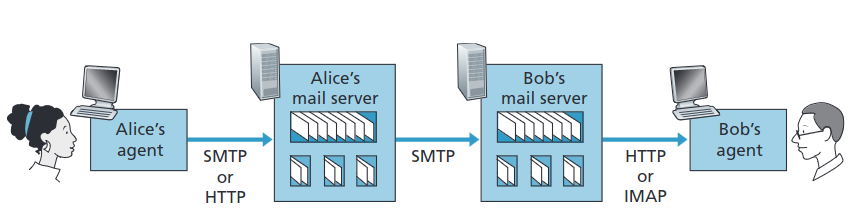
\includegraphics[width = 1\linewidth]{img/2/email-server.png}
    \caption{Protocolos de \textit{push} e \textit{pull}}
    \label{fig:email-server}
\end{figure}

\begin{itemize}
    \item Alice’s user agent uses SMTP or HTTP to deliver the e-mail
message into her mail server, then Alice’s mail server uses SMTP (as an SMTP client) to relay the e-mail message to Bob’s mail server. The two step procedure allows Alice’s mail server to repeatedly try to send the message to Bob’s mail server, until Bob’s mail server becomes operational.

    \item On the other hand, if Bob is using Web-based e-mail or a smartphone app (such as Gmail), then the user agent will use HTTP (since obtaining the messages is a pull operation, whereas SMTP is a push protocol) to retrieve Bob’s e-mail. This case requires Bob’s mail server to have an HTTP interface as well as an SMTP interface (to communicate with Alice’s mail server).
\end{itemize}

\noindent The alternative method, typically used with mail clients such as Microsoft Outlook, is to use the Internet Mail Access Protocol (IMAP). Both the HTTP and IMAP approaches allow Bob to manage folders, maintained in Bob’s mail server.
\renewcommand*{\thefootnote}{\fnsymbol{footnote}}
\footnotetext[4]{%
    \noindent \textbf{Internet Message Access Protocol (IMAP):} managing and accessing email messages on a remote.
    
    \vspace{-1em}
    \begin{enumerate}
        \item \textbf{Server-based Storage:} IMAP stores email messages on a remote server, allowing users to access their emails from multiple devices without needing to download messages locally.
        \item \textbf{Folder Organization:} Users can create, rename, and delete folders to organize their emails.
        \item \textbf{Selective Retrieval:} IMAP supports downloading only email headers or specific parts of a message, conserving bandwidth and improving efficiency.
        \item \textbf{Synchronization:} Changes made to emails, such as marking messages as read or moving them between folders, are synchronized with the server, ensuring a consistent view across all devices.
    \end{enumerate}
}
\renewcommand*{\thefootnote}{\arabic{footnote}}
%//==============================--@--==============================//%
        \clearpage
%//==============================--@--==============================//%
\subsection[2.4 Domain Name System (DNS)]{\hspace*{0.075 em}\raisebox{0.2 em}{$\pmb{\drsh}$} Domain Name System (DNS)}
\label{subsec:dns}

The Domain Name System (DNS) is a hierarchical and distributed database that translates human-readable domain names (e.g., \url{www.example.com}) into their corresponding IP addresses, which are used by computers to communicate with each other. This translation is \underline{essential for} the functioning of \underline{the Internet}.

%//==============================--@--==============================//%
\subsubsection[2.4.1 Services Provided by DNS]{$\pmb{\rightarrow}$ Services Provided by DNS}

DNS provides various services, including:

\vspace{-0.5em}
\begin{enumerate}
    \item \textbf{Hostname-to-IP address translation:} The primary function of DNS is to translate domain names into their corresponding IP addresses.
    \item \textbf{Alias resolution:} DNS allows the use of aliases (alternative domain names) to reference the same IP address. This is helpful for load balancing and providing user-friendly names.
    \item \textbf{Reverse lookup:} DNS can perform a reverse lookup, \underline{converting an IP} address back into its \underline{corresponding domain name}.
    \item \textbf{Load distribution:} DNS can distribute the load among multiple servers by returning different IP addresses for the same domain name.
\end{enumerate}

%//==============================--@--==============================//%
\subsubsection[2.4.2 Overview of how DNS works]{$\pmb{\rightarrow}$ Overview of how DNS works}

DNS operates using a distributed hierarchy of servers organized into four levels:

\vspace{-0.5em}
\begin{enumerate}
    \item \textbf{Root DNS servers:} These servers are at the top of the hierarchy and provide information about top-level domains (e.g., .com, .org).
    \item \textbf{Top-level domain (TLD) servers:} These servers are responsible for specific top-level domains, such as .com or .org, and provide information about second-level domains (e.g., example.com).
    \item \textbf{Authoritative DNS servers:} These servers store the actual DNS records for specific domain names and are responsible for providing the IP address associated with a given domain name.
    \item \textbf{Local DNS servers:} These servers are operated by ISPs or organizations and are the first point of contact for end-user DNS queries. They cache query results to provide faster responses for future requests.
\end{enumerate}

\noindent When a user requests the IP address for a domain name, the local DNS server initiates a series of queries through the DNS hierarchy until it reaches the authoritative DNS server for the requested domain, which provides the IP address.

\begin{figure}[H]
    \begin{subfigure}[b]{0.5\linewidth}%
        \centering
        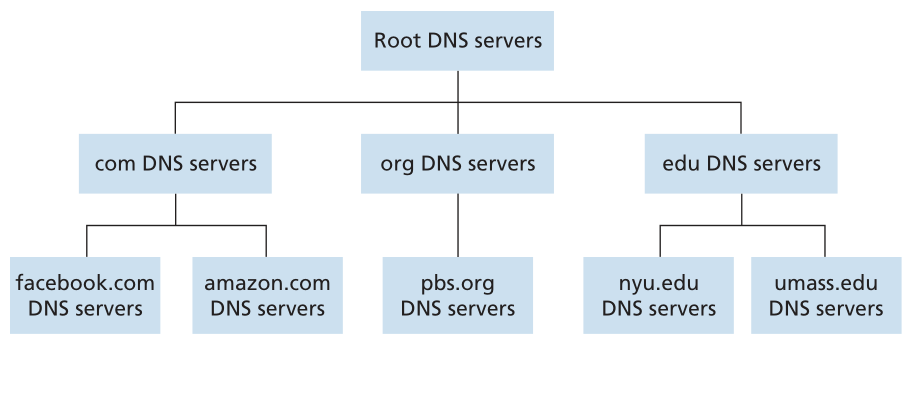
\includegraphics[width = 1\linewidth]{img/2/dns-hierarchy.png}
        \caption{``Portion of the hierarchy of DNS servers''\protect\cite{Kurose2017}}
        \label{fig:dns-hierarchy}
    \end{subfigure} \hfill
    \begin{subfigure}[b]{0.5\linewidth}%
        \centering
        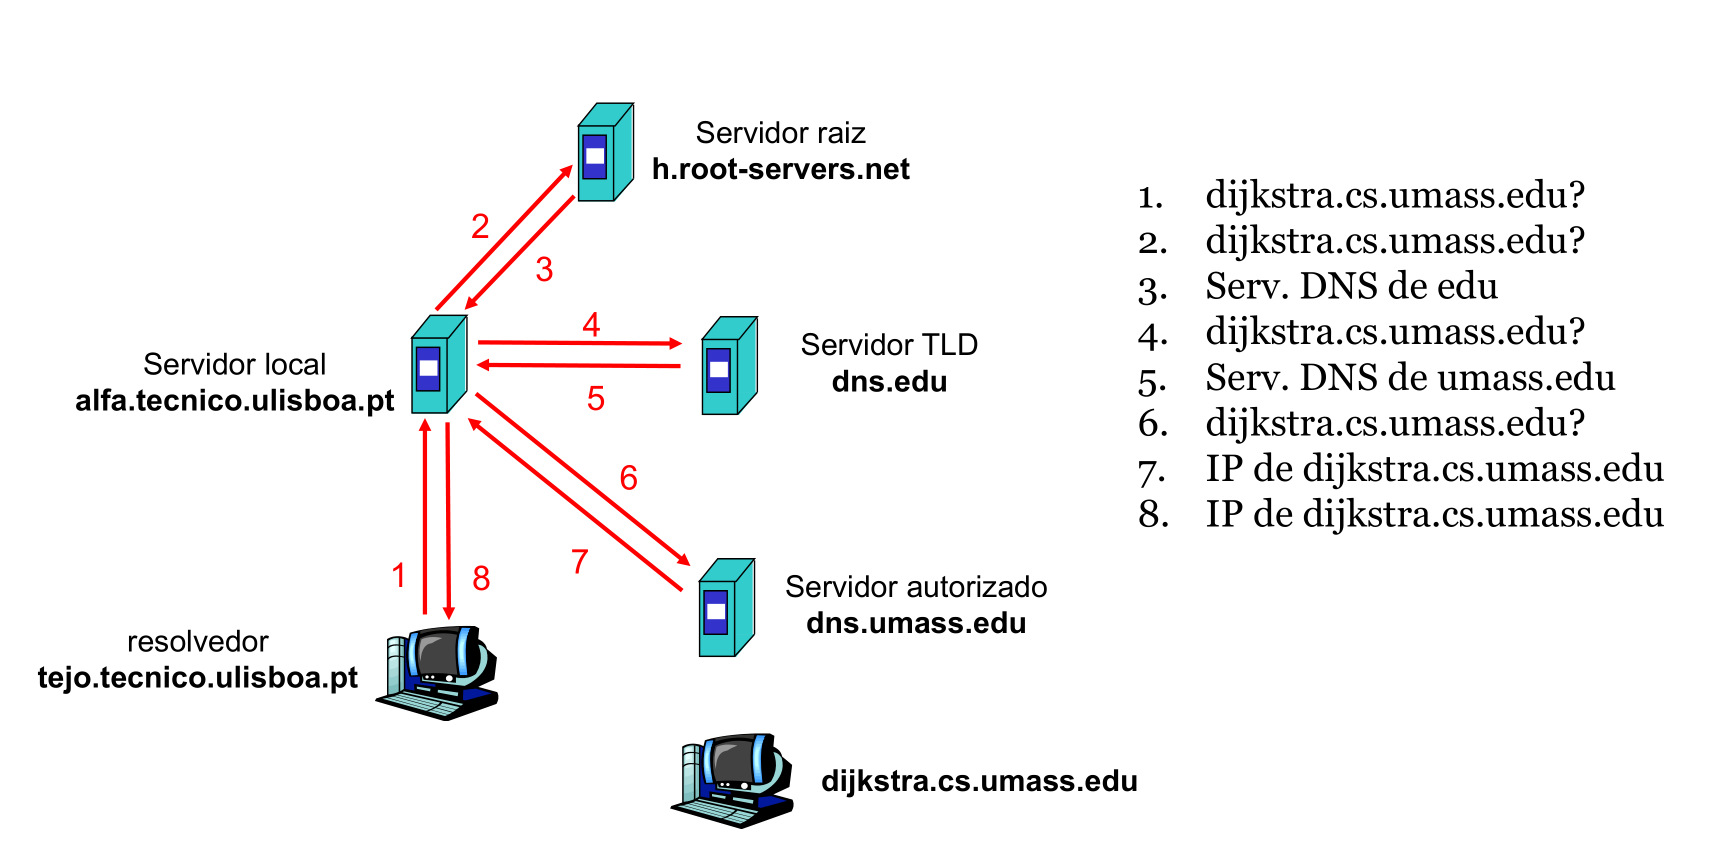
\includegraphics[width = 1\linewidth]{img/2/dns-hierarchy-example.png}
        \caption{``DNS: exemplo''\protect\cite{slidesSobrinho}}
        \label{fig:dns-hierarchy-example}
    \end{subfigure}%
    \caption{DNS hierarchy overview}
\end{figure}

%//==============================--@--==============================//%
\subsubsection[2.4.3 DNS records and messages]{$\pmb{\rightarrow}$ DNS records and messages}

DNS uses \textbf{Resource Records} (RRs) to store information. The most common RR types are:

\vspace{-0.5em}
\begin{enumerate}
    \item \textbf{A:} Contains the IP address corresponding to a given domain name.
    \item \textbf{NS:} Specifies the authoritative name server for a domain.
    \item \textbf{CNAME:} Defines an alias for a domain name, allowing multiple names to reference the same IP address.
    \item \textbf{MX:} Indicates the mail exchange server responsible for handling email for a domain.
    \item \textbf{PTR:} Provides reverse lookup functionality, mapping an IP address back to a domain name.

\end{enumerate}

\begin{lstlisting}[language=, title={Exemplo de registo de recursos \protect\cite{slidesSobrinho}}, frame=tb, basicstyle=\scriptsize\ttfamily, escapechar=\%]
%\begin{center} \small (Domain name, Value, Type, Classe, TTL) \end{center}%

(tejo.tecnico.ulisboa.pt, 193.136.138.142, A, IN, 448)
(tejo.tecnico.ulisboa.pt, 2001:CD00:0:CDE:1257:0:211E:729C, AAAA, IN, 448)
(tecnico.ulisboa.pt, ns1.tecnico.ulisboa.pt, NS, IN, 3600)
(mae.princeton.edu, live-princeton-mae-next.pantheonsite.io, CNAME, IN, 86400)
(tecnico.ulisboa.pt, email.tecnico.ulisboa.pt, MX, IN, 3600)
\end{lstlisting}

\vskip 0.5em
\noindent DNS messages consist of two types of messages:

\vspace{-0.5em}
\begin{enumerate}
    \item \textbf{Query:} A message sent by a client (local DNS server) to a DNS server, requesting the resolution of a domain name or an IP address.
    \item \textbf{Response:} A message sent by the DNS server back to the client, containing the requested information (e.g., IP address or domain name) and any additional relevant records.
\end{enumerate}

\noindent Both query and response messages have the same format, consisting of a header and four sections: Question, Answer, Authority, and Additional Information. The header contains various flags and identifiers, while the four sections contain the relevant resource records and requested information.

\begin{figure}[H]
    \centering
    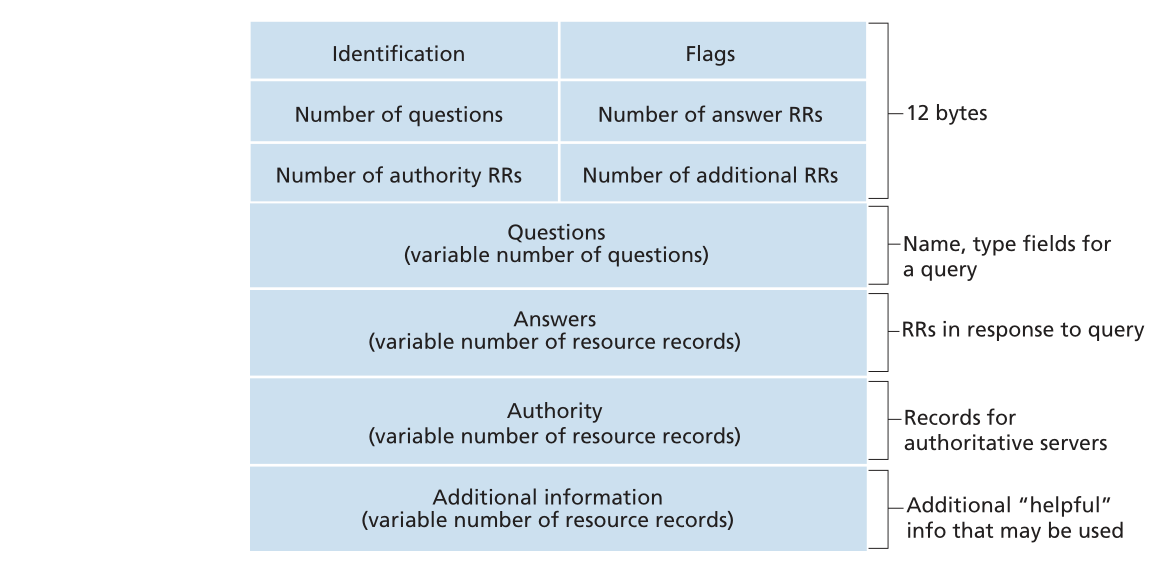
\includegraphics[width = 0.8\linewidth]{img/2/dns-message-format.png}
    \caption{``DNS message format''\protect\cite{Kurose2017}}
    \label{fig:dns-message-format}
\end{figure}

\renewcommand*{\thefootnote}{\fnsymbol{footnote}}
\footnotetext[4]{%
``\texttt{TTL} is the Time-To-Live of the resource record; it determines when a resource should be removed from a cache.''\cite{Kurose2017}
}
\renewcommand*{\thefootnote}{\arabic{footnote}}

%//==============================--@--==============================//%
\subsubsection[2.4.4 DNS Caching and Query Resolution]{$\pmb{\rightarrow}$ DNS Caching and Query Resolution}


\begin{enumerate}
    \item \textbf{DNS Caching:} Temporarily storing DNS query results to reduce lookup times for subsequent requests.
    \begin{enumerate}
            \item \textbf{Local Cache:} DNS clients (resolvers) and recursive DNS servers store query results locally to quickly answer repeated requests.
            \item \textbf{Cache Expiration:} Each DNS record has a Time-To-Live (TTL) value determining how long it should be stored in a cache before being discarded.
    \end{enumerate}
    
    \item \textbf{Recursive Query:} A DNS server contacts other DNS servers on behalf of the client to resolve a query, returning the final result to the client.
    
    \item \textbf{Iterative Query:} A DNS server provides the client with a referral to another DNS server, and the client continues the query resolution process by contacting the referred server.
\end{enumerate}

%//==============================--@--==============================//%
        %//==============================--@--==============================//%
\subsection[2.5 Socket Programming: Aplicações de Rede]{\hspace*{0.075 em}\raisebox{0.2 em}{$\pmb{\drsh}$} Socket Programming: Aplicações de Rede}
\label{subsec:socket-programming}

Uma aplicação de rede é tipicamente constituída por um par de programas---um programa de \textit{cliente} e um programa de \textit{servidor}---que residem em sistemas terminais distintos. Quando estes programas são executados, é iniciado um \textit{processo de cliente} e um \textit{processo de servidor}, que comunicam entre si ao ler e escrever em \textbf{\textit{sockets}}.

\begin{theo}[\underline{Socket}]{def:socket}\label{def:socket}
    {\footnotesize
        ``A \textbf{network socket} is a software structure within a network node of a computer network that serves as an endpoint for sending and receiving data across the network. The structure and properties of a socket are defined by an application programming interface (API) for the networking architecture. Sockets are created only during the lifetime of a process of an application running in the node. The API for the network protocol stack creates a handle for each socket created by an application, commonly referred to as a \textit{socket descriptor}.''
    }

    \vspace{0.75em}
    \noindent As \textit{sockets} são uma abstração que permite comunicar entre sistemas terminais com o uso de \textit{socket descriptors} standard. Em sistemas UNIX, todas as ações \texttt{I/O} são realizadas ao escrever, e ler, em \textit{file descriptors}.
\end{theo}

%\vspace{-1em}
\begin{figure}[H]
    \centering
    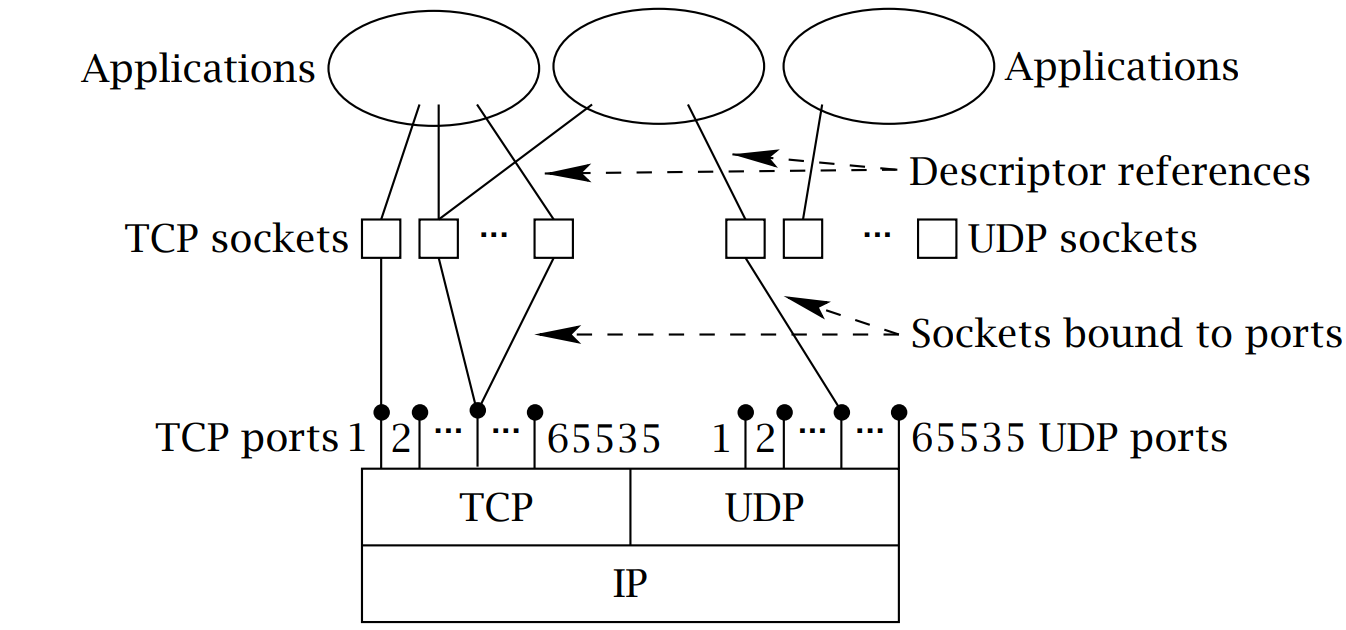
\includegraphics[width = 0.75\linewidth]{img/2/app-sockets-protocols.png}
    \caption{``Logical relationships among applications, socket abstractions, protocols, and port numbers within a single host.''\protect\cite{Donahoo-Kenneth2002}}
    \label{fig:app-sockets-protocols}
\end{figure}

\renewcommand*{\thefootnote}{\fnsymbol{footnote}}
\footnotetext[4]{%
    \textbf{Nota:} Um \textit{file descriptor} (\texttt{fd}) é um inteiro associado a um ficheiro aberto que pode ser: uma conexão de rede, um ficheiro de texto, um terminal...
}
\renewcommand*{\thefootnote}{\arabic{footnote}}

%//==============================--@--==============================//%
\iffalse
\clearpage
\subsubsection[2.5.1]{$\pmb{\rightarrow}$ Socket Programming: UDP}

\begin{lstlisting}[title={UDP\_client.c}]
#include <unistd.h>
#include <stdlib.h>
#include <string.h>
#include <sys/types.h>
#include <sys/socket.h>
#include <netinet/in.h>
#include <arpa/inet.h>
#include <netdb.h>

#define PORT "58001"

int main(void) {
	int fd, errcode;
	ssize_t n;
	socklen_t addrlen;
	struct addrinfo hints, *res;
	struct sockaddr_in addr;
	char buffer[128];

	fd = socket(AF_INET,SOCK_DGRAM,0); //UDP socket
	if (fd == -1) /*error*/ exit(1);

	memset(&hints,0,sizeof(hints));
	hints.ai_family = AF_INET;         //IPv4
	hints.ai_socktype = SOCK_DGRAM;    //UDP socket

	errcode = getaddrinfo("tejo.tecnico.ulisboa.pt",PORT,&hints,&res);
	if (errcode != 0) /*error*/ exit(1);

	n = sendto(fd,"Hello!\n",7,0,res->ai_addr,res->ai_addrlen);
	if (n == -1) /*error*/ exit(1);

	addrlen = sizeof(addr);
	n = recvfrom(fd,buffer,128,0,(struct sockaddr*) &addr, &addrlen);
	if (n == -1) /*error*/ exit(1);
	write(1,"echo: ",6); write(1,buffer,n);

	freeaddrinfo(res);
	close(fd);
}
\end{lstlisting}

%//==============================--@--==============================//%
\subsubsection[2.5.2]{$\pmb{\rightarrow}$ Socket Programming: TCP}

%//==============================--@--==============================//%
\fi

    \clearpage\addtocontents{toc}{\protect\newpage}
    \section{3. Camada de Transporte}\label{sec:transport-layer}%
        %//==============================--@--==============================//%
\subsection[3.1 Visão Geral]{\hspace*{0.075 em}\raisebox{0.2 em}{$\pmb{\drsh}$} Visão Geral}
\label{subsec:overview}

\begin{quote}
    ``Recall that the transport layer lies just above the network layer in the protocol stack. Whereas a\textbf{ transport-layer protocol provides logical communication between processes}  running on different hosts, a \textbf{network layer protocol provides logical communication between hosts}.''\cite{Kurose2017}
\end{quote}

\begin{figure}[H]
    \centering
    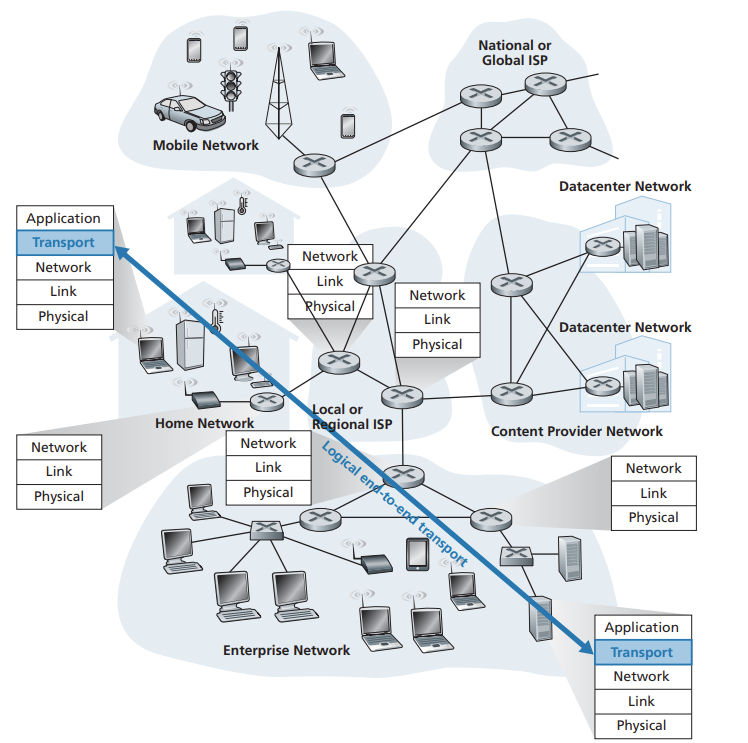
\includegraphics[width = 0.7\linewidth]{img/3/logical-transport.png}
    \caption{``Logical communication between processes''\protect\cite{Kurose2017}}
    \label{fig:logical-transport}
\end{figure}

\noindent A camada de transporte fornece uma abstração sobre a comunicação entre aplicações (processos) que atuam em \textit{hosts} diferentes---``It allows for communication between processes running on different hosts as if they were directly connected, even if they are physically located on opposite sides of the planet''\cite{Kurose2017}. A camada de rede garante o fluxo de \textit{packets} de um \textit{host} a outro, iterando sobre um número arbitrário de redes.

\vspace{0.5 em}
\noindent ``Recall that the Internet makes two distinct transport-layer protocols available to the application layer. One of these protocols is \textbf{UDP} (User Datagram Protocol) and \textbf{TCP} (Transmission Control Protocol)":

\begin{itemize}
    \item \textbf{Entrega fiável e ordenada para unicast: TCP}
    \vspace{-0.25em}    
    \begin{itemize}
        \item Controlo de erros
        \item Controlo de fluxo
        \item Controlo de congestão
    \end{itemize}
    
    \item \textbf{Entrega não-fiável para unicast ou multicast: UDP}
    \vspace{-0.25em}
    \begin{itemize}
        \item Deteção de erros
    \end{itemize}
\end{itemize}

\clearpage
\begin{quote}
    ``Transport-layer protocols are implemented in the end systems but not in network routers. On the sending side, the transport layer converts the application-layer messages it receives from a sending application process into transport-layer packets, known as transport-layer \textbf{segments} in Internet terminology. This is done by (possibly) breaking the application messages into \textbf{smaller chunks} and adding a \textbf{transport-layer header to each chunk} to create the \textbf{transport-layer segment}. The transport layer then passes the segment to the network layer at the sending end system, where the segment is encapsulated within a network-layer packet (a datagram) and sent to the destination.''\cite{Kurose2017}
\end{quote}


%//==============================--@--==============================//%
        %//==============================--@--==============================//%
\subsection[3.2 Multiplexação e Desmultiplexaçãol]{\hspace*{0.075 em}\raisebox{0.2 em}{$\pmb{\drsh}$} Multiplexação e Desmultiplexação}
\label{subsec:multiplex-demultiplex}


\begin{theo}[\underline{Multiplexing and demultiplexing}]{teo/def:Multi-Demu}\label{def:Multi-Demu}
    ``At the destination host, the transport layer receives segments from the network layer just below. The transport layer has the responsibility of delivering the data in these segments to the appropriate application process (socket) running in the host. (...) \textbf{This job of delivering the data in a transport-layer segment to the correct socket is called} \textbf{demultiplexing}. \textbf{The job of gathering data chunks at the source host from different sockets, encapsulating each data chunk with header information to create segments}, and passing the segments to the network layer \textbf{is called multiplexing}" 
\end{theo}

\noindent A multiplexação e a desmultiplexação está dependente da identificação única inerente às \textit{sockets} e requer que cada segmento da camada de transporte possua um \textbf{source port number} field e um \textbf{destination port number} field (\textit{vide} \hyperref[appendixB]{Appendix C: Reserved Ports}).

\begin{figure}[H]
    \centering
    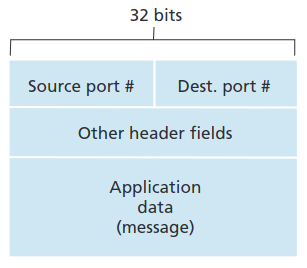
\includegraphics[width = 0.45\linewidth]{img/3/segment.png}
    \caption{Estrutura de um segmento da camada de transporte.\protect\cite{Kurose2017}}
    \label{fig:segment}
\end{figure}

\noindent Os restantes \textit{header fields} estão dependentes do tipo de protocolo em uso, nomeadamente, \textbf{UDP} e \textbf{TCP}.

%//==============================--@--==============================//%
        \clearpage
%//==============================--@--==============================//%
\subsection[3.3 Connectionless Transport: UDP]{\hspace*{0.075 em}\raisebox{0.2 em}{$\pmb{\drsh}$} Connectionless Transport: UDP}
\label{subsec:UDP}

\noindent \textbf{Nota:} As sockets UDP são identificada somente por dois campos: porto de destino e endereço IP de destino. Tal significa que informação oriunda de dois \textit{hosts} diferentes (consequentemente IP's de origem diferentes) cujos destinos possuem o mesmo IP e o mesmo porto será recebida pela mesma \textit{socket}.

\vspace{1 em}
\noindent A estrutura de um segmento UDP é a seguinte:

\begin{figure}[H]
    \centering
    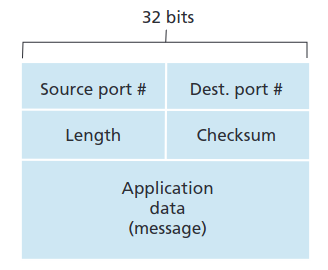
\includegraphics[width = 0.5\linewidth]{img/3/UDP-segment.png}
    \caption{Estrutura de um segmento UDP}
    \label{fig:seg-UDP}
\end{figure}

\begin{itemize}
    \item The UDP header has only four fields, each consisting of two bytes.
    \item The port numbers allow the destination host to pass the application data to the correct process running on the destination end system (that is, to perform the demultiplexing function).
    \item The length field specifies the number of bytes in the UDP segment (header plus data). An explicit length value is needed since the size of the data field may differ from one UDP segment to the next.
    \item The checksum is used by the receiving host to check whether errors have been introduced into the segment (como já referido, o protocolo garante apenas deteção de erros).
\end{itemize} 

%//==============================--@--==============================//%
\subsubsection[3.3.1 Checksum]{$\pmb{\rightarrow}$ Checksum}
\label{subsubsec:checksum}

\begin{mdframed}
    \begin{center}
        \textbf{Checksum (soma de verificação):} $\overline{x_1 \oplus \dots \oplus x_m} = 2^n - 1 - \left(x_1 \oplus \dots \oplus x_m \right)$
    \end{center}
    \vspace{-0.5em}
    \begin{quote}
        ``$[$The$]$ Sender side performs the 1s complement of the sum of all the 16-bit words in the segment"\cite{Kurose2017}
    \end{quote}
\end{mdframed}

\begin{quote}
    ``The UDP checksum provides for error detection. That is, \textbf{the checksum is used to determine whether bits within the UDP segment have been altered} (for example, by noise in the links or while stored in a router) as it moved from source to destination."\cite{Kurose2017}
\end{quote}

\noindent \underline{\textbf{Relembrar}}: Soma binária com \textit{wrapping} em caso de \textit{overflow}
$$
    x \oplus y = 
    \begin{cases}
        x + y, & x + y < 2^n \\
        x + y - 2^n + 1, &  x + y \ge 2^n
    \end{cases}
$$

\newpage
\noindent \textbf{Exemplo:} Supondo um segmento composto por 3 palavras de 16 bits. 

\begin{center}\texttt{%
    0110011001100000 \\
    0101010101010101 \\
    1000111100001100
    }
\end{center}

\begin{figure}[H]
    \centering
    \begin{minipage}{0.45\linewidth}%
        \begin{center}
        The sum of first two words is: \\[6pt]
        
        \texttt{%
            0110011001100000 \\
            0101010101010101 \\
            ------------------------------- \\
            1011101110110101
        }
        \end{center}
    \end{minipage}
    \raisebox{0.25em}{$\pmb{\rightarrow}$}
    \begin{minipage}{0.45\linewidth}%
        \begin{center}
        Adding the third word gives: \\[6pt]
        
        \texttt{%
            1011101110110101 \\
            1000111100001100 \\
            ------------------------------- \\
            0100101011000010
        }
        \end{center}
    \end{minipage}
    \label{fig:checksum}
\end{figure}

\vspace{-1.25
em}
$$
   \pmb{\therefore} \text{The 1s complement of the sum \texttt{0100101011000010} is \underline{\texttt{1011010100111101}}}
$$

\noindent Lastly, ``At the \textbf{receiver}, all \underline{four} 16-bit words are added $[$the segment's words and the checksum$]$. If no errors are introduced into the packet, then clearly the sum at the receiver will be \texttt{1111111111111111}."\cite{Kurose2017}

\vspace{0.75em}
\noindent \textbf{Nota:} Neste exemplo, a ultima soma resulta num \textit{overflow} que sofre um \textit{wrap around}, i.e., o bit de excesso é somado ao bit menos significativo do resultado. 
%//==============================--@--==============================//%
        %//==============================--@--==============================//%
\subsection[3.4 Reliable Data Transfer]{\hspace*{0.075 em}\raisebox{0.2 em}{$\pmb{\drsh}$} Reliable Data Transfer}
\label{subsec:reliable-data-transfer}

%//==============================--@--==============================//%
\subsubsection[3.4.1 Stop-and-Wait]{\hspace*{0.075 em}\raisebox{0.2 em}{$\pmb{\rightarrow}$} Stop-and-Wait}
\label{subsec:stop-and-wait}

Stop-and-wait is a simple and fundamental technique for reliable data transfer. The sender transmits a single data packet and then waits for an acknowledgment (ACK) from the receiver before transmitting the next packet.

\vspace{-0.5em}
\begin{enumerate}
    \item \textbf{Packet numbering}: To detect and discard duplicate packets, both data packets and ACKs are numbered. The receiver can then distinguish between new packets and duplicates.
    
    \item \textbf{Error detection}: Both data packets and ACKs include a checksum for error detection. If the receiver detects an error in a packet, it discards the packet without sending an ACK, prompting the sender to retransmit the packet.
    
    \item \textbf{Timeout and retransmission}: The sender sets a timer after transmitting a packet. If the timer expires before receiving an ACK, the sender assumes the packet or the ACK was lost and retransmits the packet.
\end{enumerate}

\begin{quote}
    ``If we define the utilization of the sender (or the channel) as the fraction of time the sender is actually busy sending bits into the channel, $[$direct observation$]$ (...) shows that the stop-and-wait protocol has a rather \textbf{dismal sender utilization} (...)''\cite{Kurose2017}
    $$
        U_\text{sender} = \frac{L/R}{\text{RTT} + L/R} \ll 1
    $$
\end{quote}

\noindent The solution to this \textit{conundrum} is known as \textbf{pipelining} as discussed bellow, where two basic approaches toward pipelined error recovery can be identified.

%//==============================--@--==============================//%
\subsubsection[3.4.2 Cumulative ACKs and Selective ACKs]{\hspace*{0.075 em}\raisebox{0.2 em}{$\pmb{\rightarrow}$} Cumulative ACKs and Selective ACKs}
\label{subsec:cumulative-acks-selective-acks}

\vspace{-0.5em}
\begin{enumerate}
    \item \textbf{Cumulative ACKs}: In this approach, the receiver acknowledges the receipt of all consecutive, correctly received packets up to a specified sequence number by sending an \underline{ACK containing the sequence number of the next expected packet}. If a packet is lost or arrives out of order, the receiver sends an ACK with the sequence number of the first expected packet it has not received.
    
    \item \textbf{Selective ACKs}: With selective ACKs, the receiver explicitly acknowledges \underline{individual packets}, allowing the sender to retransmit only the missing packets. This approach improves efficiency, especially in scenarios with high packet loss or long round-trip times.
\end{enumerate}

%//==============================--@--==============================//%
\subsubsection[3.4.3 Sliding Window Protocol]{$\pmb{\rightarrow}$ Sliding Window Protocol}

The sliding window protocol is a general concept that forms the basis for both Go-Back-N (GBN) and Selective Repeat (SR) protocols. It allows the sender to transmit multiple packets without waiting for an acknowledgment (ACK) for each one. The sender maintains a sending window that limits the number of unacknowledged packets, while the receiver maintains a receiving window that limits the number of out-of-order packets it can accept. The windows slide as the sender receives ACKs and the receiver receives in-order packets.
$$
    \text{\underline{Relação temporal fundamental:}} \quad \boxed{\frac{L}{c} \ll \text{RTT} < W \cdot \frac{L}{c} < Timeout}
$$

\begin{figure}[H]
    \centering
    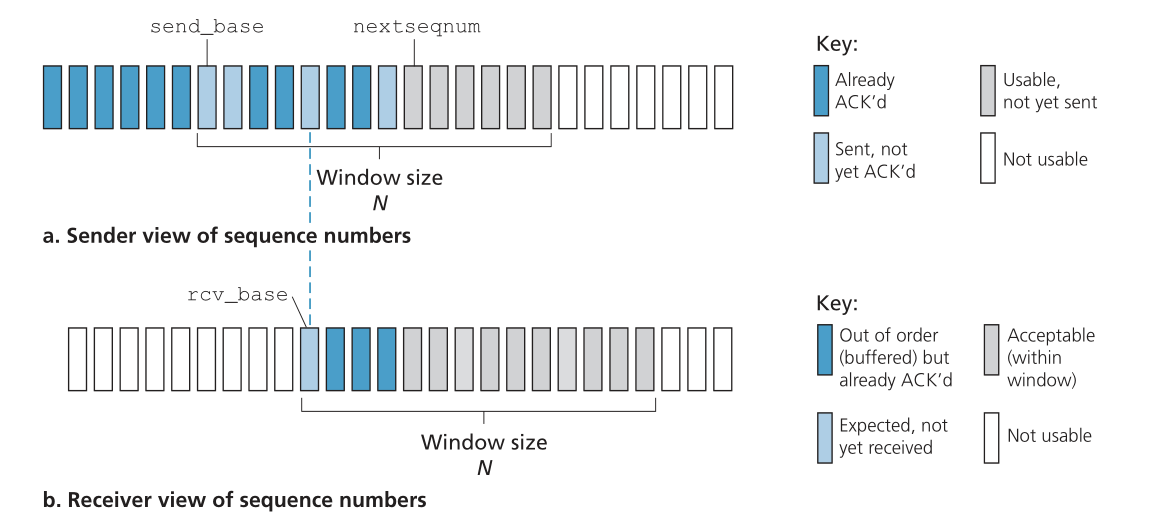
\includegraphics[width = 0.9\linewidth]{img/3/send-and-receive-windows.png}
    \caption{Exemplo janela deslizante}
    \label{fig:send-and-receive-windows}
\end{figure}

\paragraph[3.4.3.1 Go-Back-N (GBN)]{$\pmb{\star}$ Go-Back-N (GBN)}\mbox{}\\[4pt]
Go-Back-N (GBN) is a specific implementation of the sliding window protocol where the receiver sliding window has a size of 1. It uses a \underline{cumulative acknowledgment scheme}. If a packet is lost or corrupted, the receiver discards all out-of-order packets received after the lost packet. When the sender detects the loss, it retransmits the lost packet and all subsequent packets. GBN is relatively simple to implement, but its performance degrades in networks with high error rates, as it requires retransmission of multiple packets even if only a single packet was lost.
$$
    \text{\underline{Tamanho máximo da janela para evitar ambiguidades na receção:}} \quad \boxed{W_s \leq N_\text{seq} - 1}
$$

\paragraph[3.4.3.2 Temporizador/janela e ACKs cumulativos]{$\pmb{\star}$ Temporizador/janela e ACKs cumulativos}\mbox{}\\[4pt]
Uma alternativa ao protocolo GBN é a utilização de uma janela de tamanho igual à sender window no lado do receiver. Deste modo, a retransmissão de todos os pacotes subsequentes é evitada.
$$
    \text{\underline{Tamanho máximo da janela para evitar ambiguidades na receção:}} \quad \boxed{W \leq \left\lfloor N_\text{seq}/2 \right\rfloor}
$$

\paragraph[3.4.3.3 Selective Repeat (SR). Temporizador/pacote e ACKs seletivos]{$\pmb{\star}$ Selective Repeat (SR). Temporizador/pacote e ACKs seletivos}\mbox{}\\[4pt]
Selective Repeat (SR) is another implementation of the sliding window protocol, which addresses the performance issues of GBN. Instead of using cumulative ACKs, the receiver sends \underline{individual ACKs (selective ACKs)} for each received packet, regardless of their order. The receiver stores out-of-order packets in a buffer until the missing packets arrive. The sender only retransmits the lost or corrupted packets, which are identified by the absence of their respective ACKs. Although SR is more efficient than GBN in handling packet losses, it is more complex to implement due to the need to handle individual ACKs and maintain the buffer for out-of-order packets.
$$
    \text{\underline{Tamanho máximo da janela para evitar ambiguidades na receção:}} \quad \boxed{W \leq \left\lfloor N_\text{seq}/2 \right\rfloor}
$$

%//==============================--@--==============================//%
\subsubsection[3.4.4 Fast Retransmission with 3 ACKs]{\hspace*{0.075 em}\raisebox{0.2 em}{$\pmb{\rightarrow}$} Fast Retransmission with 3 ACKs}
\label{subsec:fast-retransmission}

Fast retransmission is an optimization technique to improve the performance of reliable data transfer protocols. It allows the sender to detect and retransmit lost packets faster than relying solely on timeouts.

\vspace{-0.5em}
\begin{enumerate}
    \item \textbf{Duplicate ACKs}: When the receiver detects an out-of-order packet, it sends a duplicate ACK sends an ACK with the sequence number of the first expected packet it has not received. The sender can infer that a packet was lost if it receives multiple duplicate ACKs.
    
    \item \textbf{Three-duplicate-ACKs rule}: If the sender receives three duplicate ACKs for the same packet, it assumes the packet was lost and immediately retransmits it without waiting for the timeout.
\end{enumerate}

%//==============================--@--==============================//%
\subsubsection[3.4.5 Reminder]{\hspace*{0.075 em}\raisebox{0.2 em}{$\pmb{\rightarrow}$} Reminder}
\label{subsec:reminder}

\paragraph[3.4.5.1 Canal não sequencial]{$\pmb{\star}$ Canal não sequencial}\mbox{}\\[4pt]
\noindent Mediante um canal não fiável não sequencial, o espaço de numeração deve ser tal que não existam repetições de identificadores dentro do intervalo de tempo decorrido entre a recepção do pacote mais rápido e a recepção do pacote mais lento, sendo o pacote mais lento emitido imediatamente antes do mais rápido:
$$
    \boxed{\text{número de identificadores} \ge r \cdot T}
$$
\noindent Onde $r$ é o débito a que os números de sequência são consumidos (1/delay de transmissão para \textit{sliding window protocol} e 1/RTT para \textit{stop-and-wait protocol}) e $T$ é o tempo de vida máxima de um pacote no canal.

\paragraph[3.4.5.2 Transmissão sem interrupção]{$\pmb{\star}$ Transmissão sem interrupção}\mbox{}
$$
    \boxed{ N_\text{pkt}\, t_\text{trans} \ge \text{RTT} + t_\text{trans} }
$$
%//==============================--@--==============================//%
\newpage
\subsubsection[3.4.5 TL;DR Reliable Data Transfer]{\hspace*{0.075 em}\raisebox{0.2 em}{$\pmb{\rightarrow}$} TL;DR Reliable Data Transfer}
\label{subsec:TLDR}

{
\setlength{\tabcolsep}{16pt}

\begin{table}[h!]
    \centering
    \captionsetup{justification=centering}
    \begin{tabularx}{\textwidth}{lX}
        \toprule
        \multicolumn{1}{c}{\textbf{Mechanism}} & \multicolumn{1}{c}{\textbf{Use, Comments}} \\
        \midrule
        Checksum & Used to detect bit errors in a transmitted packet. \\ \midrule
        Sequence number & Used for sequential numbering of packets of data flowing from sender to receiver. Gaps in the sequence numbers of received packets allow the receiver to detect a lost packet. Packets with duplicate sequence numbers allow the receiver to detect duplicate copies of a packet. \\ \midrule
        Acknowledgment & Used by the receiver to tell the sender that a packet or set of packets has been received correctly. Acknowledgments will typically carry the sequence number of the packet or packets being acknowledged. Acknowledgments may be individual or cumulative, depending on the protocol. \\ \midrule
        Negative acknowledgment & Used by the receiver to tell the sender that a packet has not been received correctly. Negative acknowledgments will typically carry the sequence number of the packet that was not received correctly. \\ \midrule
        Window, pipelining & The sender may be restricted to sending only packets with sequence numbers that fall within a given range. By allowing multiple packets to be transmitted but not yet acknowledged, sender utilization can be increased over a stop-and-wait mode of operation. We’ll see shortly that the window size may be set on the basis of the receiver’s ability to receive and buffer messages, or the level of congestion in the network, or both. \\
        \bottomrule
    \end{tabularx}
    \caption{``Summary of reliable data transfer mechanisms and their use''\cite{Kurose2017}}
    \label{tab:TLDR}
\end{table}
}

%//==============================--@--==============================//%
        \clearpage
%//==============================--@--==============================//%
\subsection[3.5 Connection-Oriented Transport: TCP]{\hspace*{0.075 em}\raisebox{0.2 em}{$\pmb{\drsh}$} Connection-Oriented Transport: TCP}
\label{subsec:TCP}

%//==============================--@--==============================//%
\subsubsection[3.5.1 The TCP Connection]{$\pmb{\rightarrow}$ The TCP Connection}

\begin{itemize}
    \item \textbf{Connection-oriented:} TCP establishes a connection through a \underline{handshake} before data can be exchanged between application processes.
    
    \item \textbf{Logical connection:} The TCP connection is not an end-to-end circuit but a logical one, with common state residing only in the TCPs of the communicating end systems.
    
    \item \textbf{Full-duplex service}: TCP connections allow \underline{simultaneous data flow} in both directions between two processes.
    
    \item \textbf{Point-to-point:} TCP connections only involve a single sender and a single receiver, with \underline{multicasting not possible}.
    
    \item \textbf{Three-way handshake:} To establish a TCP connection, the client and server exchange three special TCP segments, setting up the parameters for the data transfer.
    
    \item \textbf{Send and receive buffers:} Each side of the connection has its own send buffer and its own receive buffer. The client process passes a stream of data through its socket, and TCP directs this data to the connection's send buffer. From time to time, TCP grabs chunks of data from the send buffer and passes it to the network layer.
    
    \item \textbf{Maximum Segment Size (MSS):} Maximum amount of application-layer data in a segment, typically determined by the \textbf{Maximum Transmission Unit (MTU)} for the local sending host. ``Ethernet and PPP link-layer protocols have an MTU of 1,500 bytes. Thus, a typical value of MSS is 1460 bytes.''\cite{Kurose2017}
    
    \item \textbf{TCP segments:} TCP pairs each chunk of client data with a TCP header, forming TCP segments, which are passed to the network layer and encapsulated within network-layer IP datagrams.
\end{itemize}

%//==============================--@--==============================//%
\subsubsection[3.5.2 TCP Segment Structure]{$\pmb{\rightarrow}$ TCP Segment Structure}

\vspace{-0.5em}
\begin{figure}[H]
    \centering
    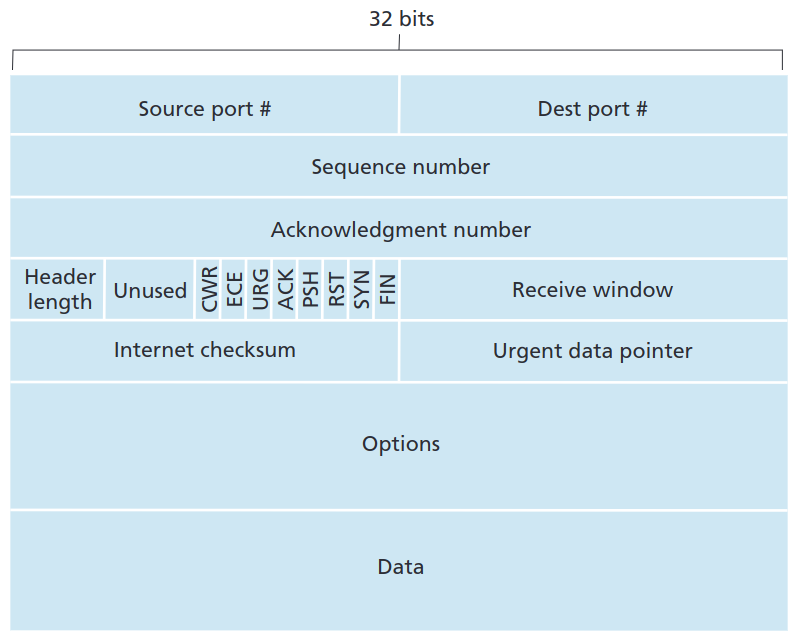
\includegraphics[width = 0.55\linewidth]{img/3/TCP-segment.png}
    \caption{Estrutura de um segmento TCP (consists of a header and payload). The header contains essential information, such as source and destination port numbers, sequence numbers, acknowledgment numbers, and flags. Additionally, the header includes the window size, checksum, and urgent pointer fields.}
    \label{fig:seg-TCP}
\end{figure}

\begin{itemize}
    \item \textbf{Sequence Numbers and Acknowledgment Numbers}
    \begin{itemize}
        \item Sequence numbers are over the stream of transmitted bytes, not over the series of transmitted segments.
        \item Acknowledgment numbers indicate the sequence number of the next byte the host is expecting.
        \item TCP provides \textbf{cumulative acknowledgments}, only acknowledging bytes up to the first missing byte in the stream.
        \item Initial sequence numbers are randomly chosen to minimize possible confusion with segments from earlier connections.
    \end{itemize}
    
    \item \textbf{Header Fields}
    \begin{itemize}
        \item \textbf{Source and destination port numbers}: for multiplexing/demultiplexing data from/to upper-layer applications.
        \item \textbf{Checksum field}
        \item 32-bit \textbf{sequence number field} and 32-bit \textbf{acknowledgment number field}: used for reliable data transfer service
        \item 16-bit \textbf{receive window field}: used for flow control, indicating the number of bytes that a receiver is willing to accept
        \item 4-bit \textbf{header length field}: specifies the length of the TCP header in 32-bit words
        \item \textbf{Optional} and \textbf{variable-length options field}: used for negotiating the MSS, window scaling factor, and time-stamping option
        \item \textbf{Flag field}: contains 6 bits (ACK, RST, SYN, FIN, CWR, and ECE) for various purposes
        \item \textbf{Urgent data pointer}: indicates the location of the last byte of urgent data
    \end{itemize}
\end{itemize}

%//==============================--@--==============================//%
\subsubsection[3.5.3 Round-Trip Time Estimation and Timeout]{$\pmb{\rightarrow}$ Round-Trip Time Estimation and Timeout}

\begin{mdframed}
    \vspace{-1.15 em}
    \begin{align*}
        \texttt{EstimatedRTT} &= \texttt{EstimatedRTT} \cdot (1 - \alpha) + \texttt{SampleRTT} \cdot \alpha \\
        \texttt{DeviationRTT} &= \texttt{DeviationRTT} \cdot (1 - \beta) + \left\vert\, \texttt{SampleRTT} - \texttt{EstimatedRTT}\, \right\vert \cdot \beta \\[-6pt] \cline{1-2}
        \texttt{Timeout} &= \texttt{EstimatedRTT} + 4 \cdot \texttt{DeviationRTT}
    \end{align*}
\end{mdframed}

\noindent \textbf{Nota:} Valores típicos para: $\alpha = 0.125 = 1/8$ $[$RFC 6298$]$, $\beta = 0.25 = 1/4$.

\renewcommand*{\thefootnote}{\fnsymbol{footnote}}
\footnotetext[4]{%
    ``Note that \texttt{EstimatedRTT} is a weighted average of the \texttt{SampleRTT} values. (...) this weighted average puts more weight on recent samples than on old samples. This is natural, as the more recent samples better reflect the current congestion in the network. In statistics, such an average is called an \textbf{exponential weighted moving average (EWMA)}.''\cite{Kurose2017}
}
\renewcommand*{\thefootnote}{\arabic{footnote}}

%//==============================--@--==============================//%
\subsubsection[3.5.4 Reliable Data Transfer]{$\pmb{\rightarrow}$ Reliable Data Transfer}
 
 Com base no discutido na \hyperref[subsec:reliable-data-transfer]{secção \textbf{Reliable Data Transfer}}, o protocolo utilizado pelo TCP é o \textbf{temporizador/janela e ACKs cumulativos}, possuindo também uma forma rudimentar de controlo de congestão que passa pela duplicação dos intervalos de \textit{timeout}: ``(...) each time TCP retransmits, it sets the next timeout interval to twice the previous value $[$sofre um crescimento exponencial$]$ (...) However, whenever the timer is started after data is received from the application above or an ACK is received, the \texttt{TimeoutInterval} is derived from the most recent values of \texttt{EstimatedRTT} and \texttt{DeviationRTT}."\cite{Kurose2017}

%//==============================--@--==============================//%
\subsubsection[3.5.5 TCP Flow Control]{$\rightarrow$ TCP Flow Control}

TCP flow control prevents sender-induced buffer overflow at the receiver, ensuring efficient data transmission. It uses a sliding window mechanism to adjust the transmission rate according to the receiver's buffer capacity and network conditions.

\vspace{-0.5em}
\begin{enumerate}
    \item \textbf{Receiver buffer and advertised window (\texttt{rwnd})}: The receiver allocates a buffer, with spare room defined as:
          \begin{equation*}
            \texttt{rwnd} = \texttt{RcvBuffer} - [\texttt{LastByteRcvd} - \texttt{LastByteRead}]
          \end{equation*}
          The sender is informed of \texttt{rwnd} via the Window field in TCP headers.
          
    \item \textbf{Sliding window and flow control operation}: The sender adjusts its sending window based on \texttt{rwnd} and network conditions. It stops transmitting data if \texttt{rwnd} drops to zero and resumes when a non-zero \texttt{rwnd} value is received.
    
    \item \textbf{Handling zero \texttt{rwnd}}: If \texttt{rwnd} is zero and the receiver has no data or ACKs to send, the sender continues sending one-byte segments to keep the receiver updated about its buffer state.
    
    \item \textbf{Interaction with congestion control}: Flow control works with congestion control mechanisms like slow start and congestion avoidance to adapt the transmission rate to both the receiver's buffer capacity and network bandwidth.
\end{enumerate}

%//==============================--@--==============================//%
\subsubsection[3.5.6 TCP Connection Management]{$\rightarrow$ TCP Connection Management}

The connection management process is mainly driven by a three-way handshake and a four-way handshake for connection establishment and termination, respectively.

\vspace{-0.5em}
\begin{enumerate}
    \item \textbf{Three-way handshake (Connection Establishment)}: The handshake process involves three steps:
        \begin{enumerate} \small
            \item SYN: The client sends a TCP segment with the SYN (synchronize) flag set, indicating a connection request.
            \item SYN + ACK: The server responds with a segment with both the SYN and ACK (acknowledge) flags set, acknowledging the client's request and synchronizing its own sequence number.
            \item ACK: The client sends an ACK segment, confirming the establishment of the connection.
        \end{enumerate}
    \item \textbf{Data transmission}: Once the connection is established, data transmission occurs using the sliding window and congestion control mechanisms.
    \item \textbf{Four-way handshake (Connection Termination)}: The termination process involves the following steps:
        \begin{enumerate} \small
            \item FIN: The endpoint initiating the connection termination sends a segment with the FIN (finish) flag set, signaling the desire to close the connection.
            \item ACK: The other endpoint acknowledges the FIN segment with an ACK segment.
            \item FIN: The other endpoint also sends a FIN segment to indicate it is ready to close the connection.
            \item ACK: The initiating endpoint acknowledges the second FIN segment with an ACK segment, completing the termination process.
        \end{enumerate}
\end{enumerate}

\renewcommand*{\thefootnote}{\fnsymbol{footnote}}
\footnotetext[4]{%
    \textbf{TCP Connection States}: During connection management, both client and server transition through various states such as LISTEN, SYN-SENT, SYN-RECEIVED, ESTABLISHED, FIN-WAIT-1, FIN-WAIT-2, CLOSING, TIME-WAIT, CLOSE-WAIT, LAST-ACK, and CLOSED.
}
\renewcommand*{\thefootnote}{\arabic{footnote}}
%//==============================--@--==============================//
        \clearpage
%//==============================--@--==============================//%
\subsection[3.6 Congestion control]{\hspace*{0.075 em}\raisebox{0.2 em}{$\pmb{\drsh}$} Congestion control}
\label{subsec:congestion-control}

\subsubsection[3.6.1 Approaches to Congestion Control]{$\pmb{\rightarrow}$ Approaches to Congestion Control}

At the highest level, we can distinguish among congestion-control approaches by whether the network layer provides explicit assistance to the transport layer for congestion-control purposes:

\begin{itemize}
    \item \textbf{Network-assisted congestion control:} In this approach, the network layer provides explicit feedback to the transport layer about the presence of congestion. The transport layer then adjusts its sending rate accordingly. Examples of this approach include ATM's ABR (Available Bit Rate) service and Frame Relay's BECN (Backward Explicit Congestion Notification) mechanism.
    
    \item \textbf{End-to-end congestion control:} In this approach, the network layer does not provide explicit feedback to the transport layer. Instead, the transport layer uses implicit feedback, typically from dropped packets or increased end-to-end delay, to infer the presence of congestion. The transport layer then adjusts its sending rate accordingly. The congestion-control mechanism used by TCP is an example of end-to-end congestion control.
\end{itemize}

\noindent Regardless of the approach taken, most congestion-control algorithms have the following objectives:

\begin{itemize}
    \item \textbf{Maximize network utilization:} The algorithm should aim to make the best use of available network resources, ensuring that network capacity is fully utilized whenever possible.
    
    \item \textbf{Fairness:} The algorithm should allocate resources fairly among competing flows, preventing any one flow from monopolizing the network.
    
    \item \textbf{Stability:} The algorithm should be able to react to changes in network conditions and maintain stable performance, avoiding oscillations in throughput or other undesirable behavior.
\end{itemize}

\subsubsection[3.6.2 Overview TCP]{$\pmb{\rightarrow}$ Overview TCP}

\noindent TCP sender limits its send rate using a congestion window (\texttt{cwnd}), which constrains the amount of unacknowledged data in the network. TCP detects congestion through loss events, either timeouts or three duplicate ACKs. In a congestion-free network, acknowledgments indicate successful data delivery, allowing the sender to increase \texttt{cwnd} and its send rate. TCP is self-clocking since it adjusts its congestion window size based on the rate of incoming acknowledgments:
$$
    \boxed{\texttt{LastByteSent} - \texttt{LastByteAcked} \leq \min\{\texttt{cwnd}, \texttt{rcvwnd}\}}
$$

\begin{enumerate}
    \item A lost segment implies congestion, and the sender should decrease its rate (by decreasing \texttt{cwnd}).
    \item An acknowledged segment indicates the network is delivering data, so the sender can increase its rate.
    \item \textbf{Bandwidth probing}: TCP increases its rate until a loss event occurs, then decreases the rate and probes again.
\end{enumerate}


\subsubsection[3.6.3 Classic TCP congestion control]{$\pmb{\rightarrow}$ Classic TCP congestion control}

\noindent \textbf{(1) Slow Start:}
\begin{itemize}[noitemsep, nolistsep]
    \item Initial \texttt{cwnd} is 1 MSS.
    \item Sender doubles sending rate every RTT.
    \item Exponential growth ends in three cases:
    \begin{itemize}[noitemsep, nolistsep]
        \item Timeout event: sets \texttt{cwnd} to 1 and \texttt{ssthresh} to \texttt{cwnd}/2 and starts slow start anew.
        \item \texttt{cwnd} equals \texttt{ssthresh}: transitions into congestion avoidance mode.
        \item Three duplicate ACKs: fast retransmit and enters fast recovery state.
    \end{itemize}
\end{itemize}

\vspace{0.5em}
\noindent \textbf{(2) Congestion Avoidance:}
\begin{itemize}[noitemsep, nolistsep]
    \item \texttt{cwnd} is approximately half its previous value.
    \item Increases \texttt{cwnd} by 1 MSS every RTT: common approach is to increase \texttt{cwnd} by MSS/\texttt{cwnd} when a new acknowledgment arrives.
    \item Linear increase (1 MSS per RTT) ends in two cases:
    \begin{itemize}
        \item Timeout event: set \texttt{cwnd} to 1 MSS, update \texttt{ssthresh} to half the value of previous cwnd.
        \item Triple duplicate ACK event: halve \texttt{cwnd} value, update \texttt{ssthresh} to half the value of previous \texttt{cwnd}, and enter fast-recovery state.
    \end{itemize}
\end{itemize}

\vspace{0.25em}
\noindent \textbf{(3) Fast Recovery} {\footnotesize (``Fast recovery is a \underline{recommended, but not required}, component of TCP''\cite{Kurose2017})}
\begin{itemize}[noitemsep, nolistsep]
    \item In fast recovery, increase \texttt{cwnd} by 1 MSS for every duplicate ACK received for the missing segment.
    \item Upon receiving an ACK for the missing segment, enter the congestion-avoidance state and deflate \texttt{cwnd}.
    \item If a timeout event occurs, perform the same actions as in slow start and congestion avoidance:
    \begin{itemize}
        \item Set \texttt{cwnd} to 1 MSS.
        \item Set \texttt{ssthresh} to half the value of \texttt{cwnd} when the loss event occurred.
    \end{itemize}
    \item After the timeout event, transition to the slow-start state.
\end{itemize}

\begin{figure}[H]
    \centering
    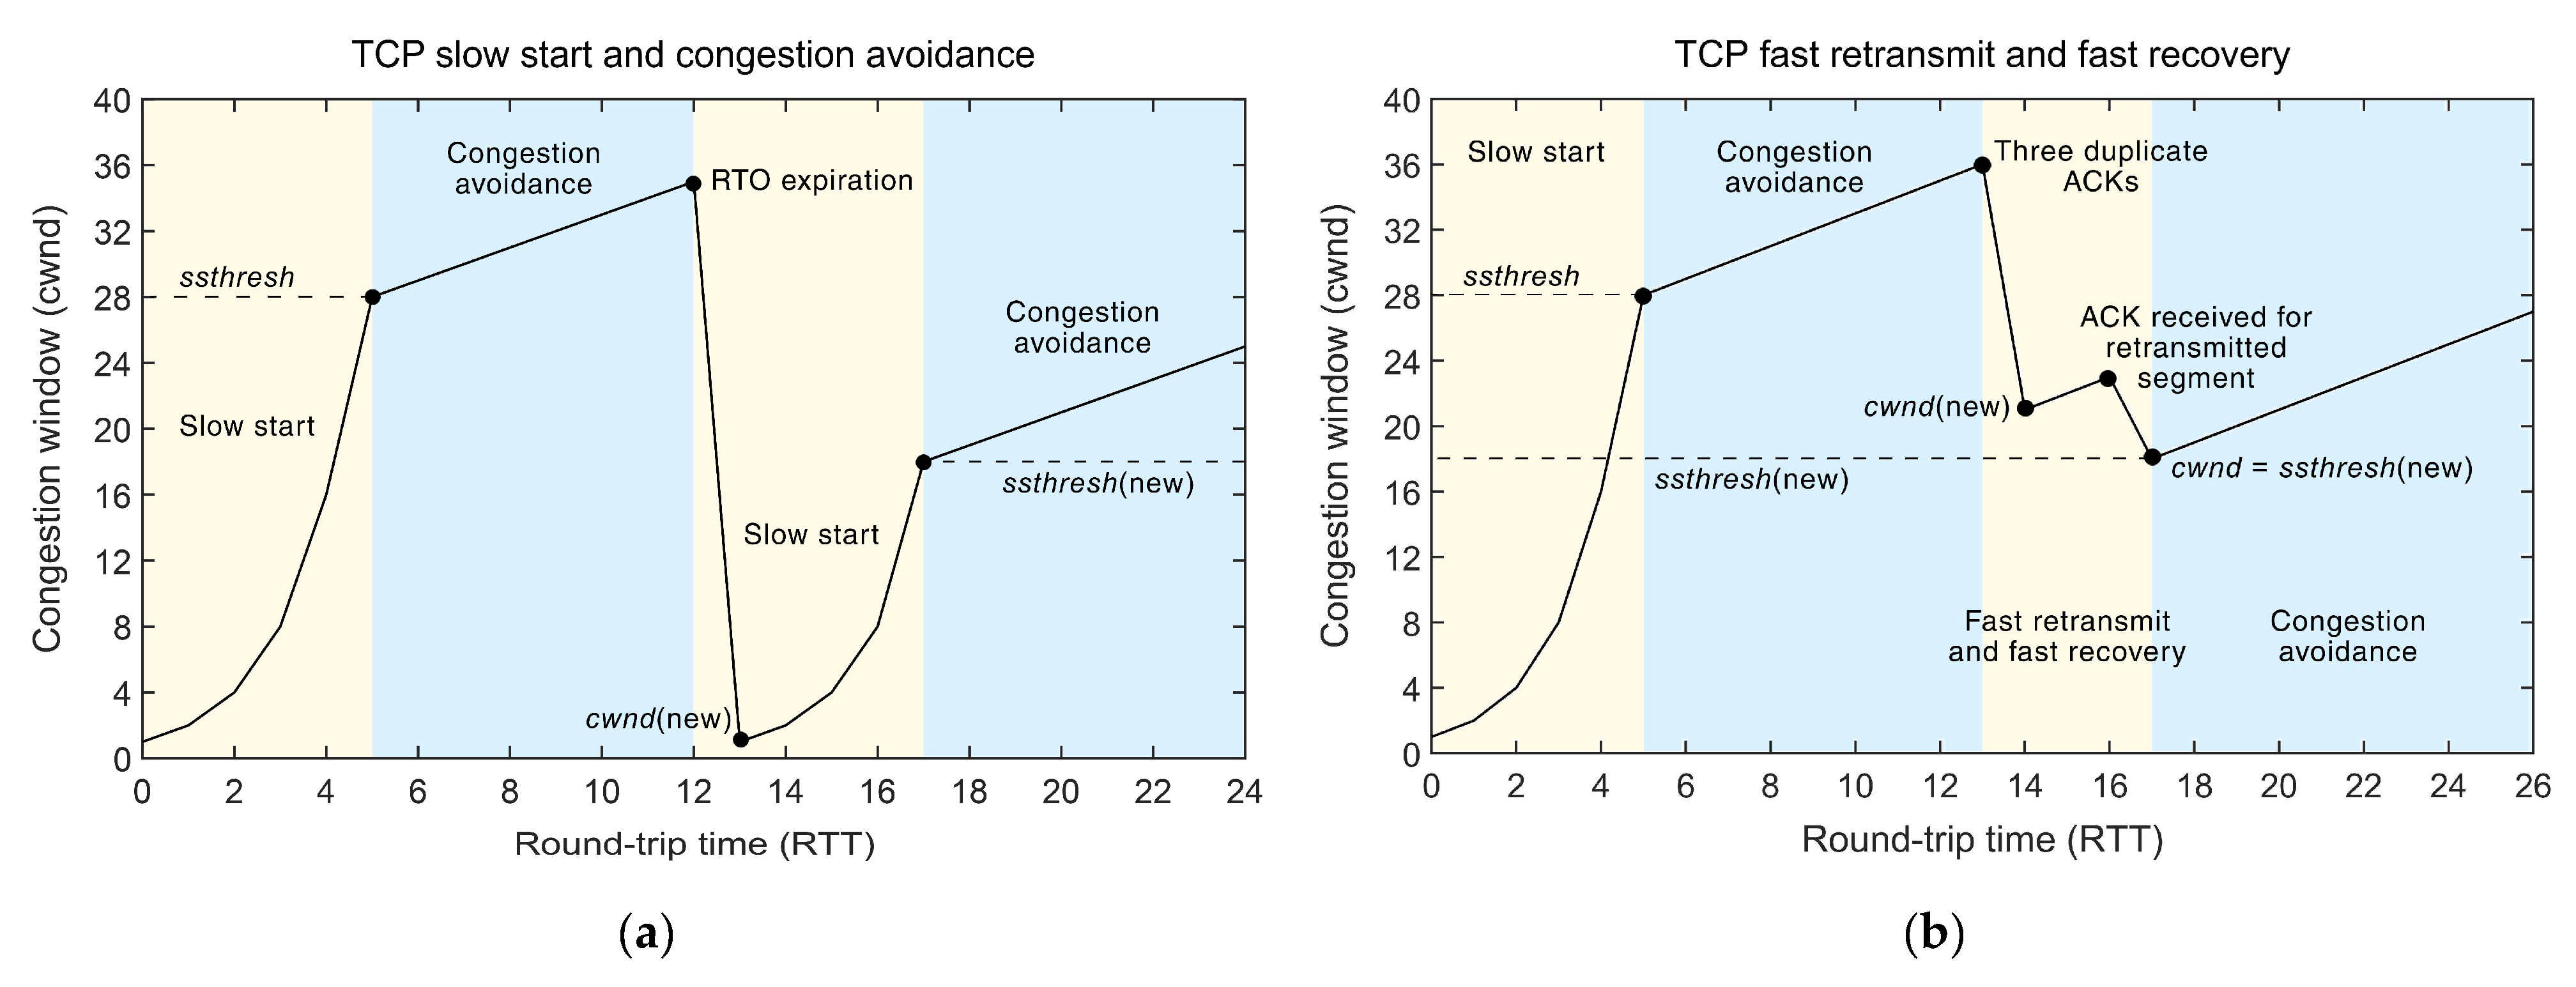
\includegraphics[width = 0.9\linewidth]{img/3/congestion-graphic.png}
    \caption{Standard working principles of the TCP CC mechanism related to the interdependence between \texttt{cwnd} and RTT for: (a) the TCP slow start and congestion avoidance mechanism; (b) the TCP fast retransmit and fast recovery mechanism. $[$Lorincz 2021$]$}
    \label{fig:congestion-graphic}
\end{figure}

\noindent ``For this reason, TCP congestion control is often referred to as an \textbf{additive-increase, multiplicative-decrease (AIMD)} form of congestion control.''\cite{Kurose2017}

\begin{figure}[H]
    \centering
    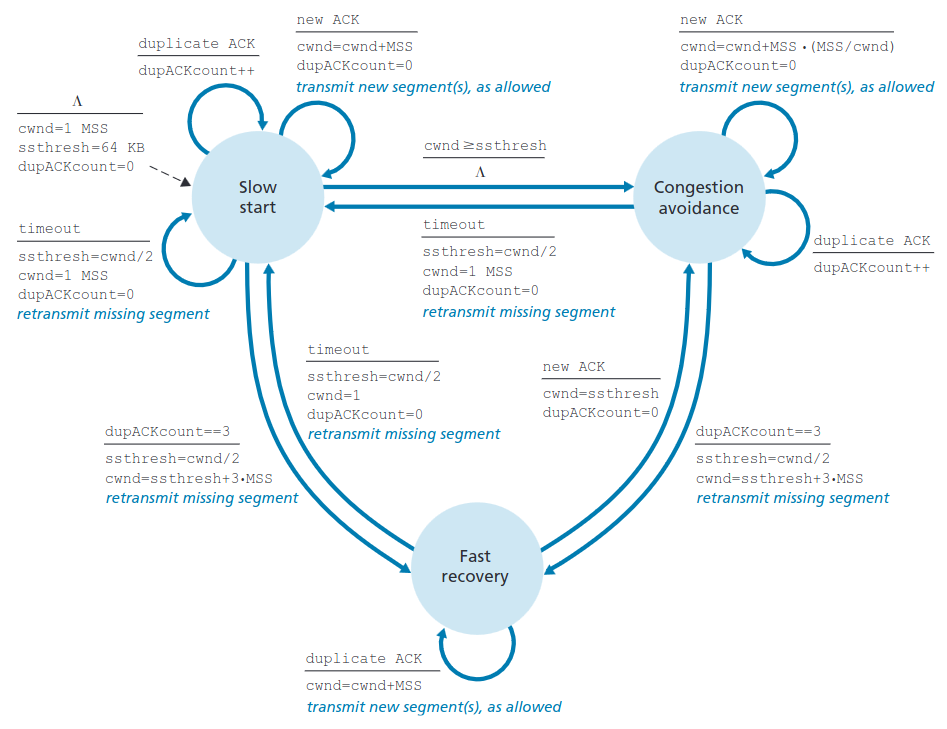
\includegraphics[width = 1\linewidth]{img/3/congestion-control-diagram.png}
    \caption{Diagrama de controlo de congestão TCP \cite{Kurose2017}}
    \label{fig:congestion-control-diagram}
\end{figure}

\paragraph[3.6.3.1 Nota histórica: TCP Tahoe \& TCP Reno]{$\pmb{\star}$ Nota histórica: TCP Tahoe \& TCP Reno}\mbox{}

\begin{figure}[ht]
    \centering
    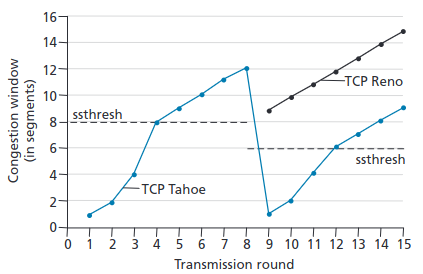
\includegraphics[width = 0.65\linewidth]{img/3/reno-tahoe.png}
    \caption{``Evolution of TCP’s congestion window (Tahoe and Reno)''\cite{Kurose2017}}
    \label{fig:tahoe-reno}
\end{figure}

\vspace{-1em}
\begin{quote}
    ``Fast recovery is a recommended, but not required, component of TCP $[$RFC 5681$]$. It is interesting that an early version of TCP, known as TCP Tahoe, unconditionally cut its congestion window to 1 MSS and entered the slow-start phase after either a timeout-indicated or triple-duplicate-ACK-indicated loss event. The newer version of TCP, TCP Reno, incorporated fast recovery.''\cite{Kurose2017}
\end{quote}

\newpage
\subsubsection[3.6.4 Extensions and Alternatives to TCP]{$\rightarrow$ Extensions and Alternatives to TCP}

\begin{itemize}
    \item \textbf{RED (Random Early Discard):} An active queue management strategy that randomly drops packets before the buffer is full, encouraging sources to reduce sending rates and preventing global synchronization of flows.
    
    \item \textbf{ECN (Explicit Congestion Notification):} A mechanism allowing routers to signal congestion to end-points by setting a flag in the packet header, allowing end-points to adjust their sending rates without waiting for packet loss as a signal.
    
    \item \textbf{TCP Vegas:} A congestion control algorithm that detects congestion early by monitoring the difference between expected and actual throughput, adjusting sending rates to avoid oscillations and maintain steady performance.
    
    \item \textbf{TCP BBR (Bottleneck Bandwidth and Round-trip propagation time):} A congestion control algorithm using the bottleneck bandwidth and round-trip time to estimate available network capacity, achieving higher throughput and lower latency than traditional loss-based algorithms.
    
    \item \textbf{CUBIC TCP:} A congestion control algorithm using a cubic function for window growth, enabling faster recovery from congestion and better performance in high-bandwidth, high-latency networks.
    
    \item \textbf{QUIC (Quick UDP Internet Connections):} A transport layer protocol developed by Google using UDP, offering faster connection establishment, built-in encryption, and improved congestion control compared to TCP, resulting in better web performance over high-latency networks.
\end{itemize}

\subsubsection[3.6.5 Congestion control fairness]{$\rightarrow$ Congestion control fairness}

Fairness in congestion control refers to the equal distribution of available bandwidth among concurrent connections. Various factors can affect the fairness of congestion control mechanisms:

\begin{itemize}
    \item \textbf{TCP's AIMD algorithm:} For TCP's AIMD algorithm, it converges to provide an equal share of a bottleneck link's bandwidth among competing TCP connections, as demonstrated by Chiu 1989. This algorithm allows TCP connections to adjust their transmission rates based on network congestion and fairly share the available bandwidth.
    
    \item \textbf{Varying RTTs:} Multiple connections sharing a common bottleneck with varying RTTs can lead to unequal bandwidth allocation. Connections with smaller RTTs can grab available bandwidth more quickly, resulting in higher throughput than connections with larger RTTs.
    
    \item \textbf{UDP vs. TCP:} Many multimedia applications often run over UDP to avoid TCP's rate throttling, leading to a potentially unfair distribution of resources. UDP sources can maintain constant transmission rates and occasionally lose packets, while TCP sources reduce their rates during congestion. As a result, UDP sources can crowd out TCP traffic, causing fairness concerns.
    
    \item \textbf{Real-world scenarios:} In real-world situations, the ideal conditions such as only TCP connections traversing the bottleneck link, connections having the same RTT value, and only a single TCP connection being associated with a host-destination pair are rarely met. As a result, these factors can lead to unequal bandwidth allocation among different connections in client-server applications.
\end{itemize}

%//==============================--@--==============================//%

    \clearpage
    \section{4. Camada de Rede}\label{sec:network-layer}%
        %//==============================--@--==============================//%
\subsection[5.1 Visão Geral]{\hspace*{0.075 em}\raisebox{0.2 em}{$\pmb{\drsh}$} Visão Geral}
\label{subsec:visao-geral}

\begin{theo}[\underline{Link Layer}]{def:Link-Layer}\label{def:Link-Layer}
    ``The basic service of any link layer is to move a datagram from one node to an adjacent node over a single communication link."\cite{Kurose2017}
\end{theo}

\noindent The link layer may provide the following services:
\begin{itemize}
    \item \textbf{Framing:} Encapsulates network-layer datagrams in link-layer frames. A frame consists of a data field, in which the network-layer datagram is inserted, and a number of header fields.
    \item \textbf{Link access:} MAC (Medium Access Control) protocol governs frame transmission, coordinating multiple nodes on a broadcast link.
    \item \textbf{Reliable delivery:} Ensures error-free transmission across the link, useful for high-error-rate links but unnecessary for low-error-rate links.
    \item \textbf{Error detection and correction:} Identifies and corrects bit errors introduced by signal attenuation and electromagnetic noise.
\end{itemize}

\noindent The link layer implementation:
\begin{itemize}
    \item Involves both hardware and software components.
    \item Uses a \textbf{network adapter}, also known as a \textbf{network interface controller (NIC)} for hardware implementation.
    \item Can be integrated into the motherboard chipset or implemented via a dedicated Ethernet chip.
    \item Handles various link layer services including framing, link access, and error detection.
\end{itemize}

\begin{figure}[H]
    \centering
    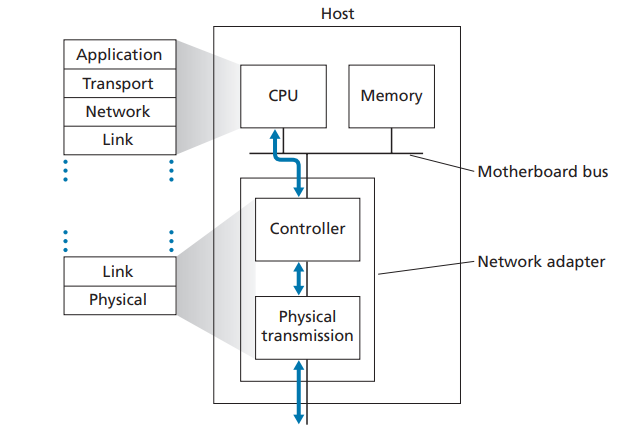
\includegraphics[width = 0.75\linewidth]{img/5/network-adapter.png}
    \caption{``Network adapter: relationship to other host components and to protocol stack functionality''\cite{Kurose2017}}
    \label{fig:network-adapter}
\end{figure}

\newpage
\noindent The link layer in the protocol stack involves both hardware and software components:
\begin{itemize}
    \item On the sending side:
    \begin{itemize}[nolistsep, noitemsep]
        \item The network adapter takes a datagram created and stored in host memory by higher layers of the protocol stack.
        \item It encapsulates the datagram in a link-layer frame.
        \item The frame is transmitted into the communication link following the link-access protocol.
    \end{itemize}
    \item On the receiving side:
    \begin{itemize}[nolistsep, noitemsep]
        \item The network adapter receives the entire frame.
        \item It extracts the network-layer datagram.
        \item Error detection is performed, if necessary.
    \end{itemize}
    \item Higher-level link-layer features are implemented in software running on the host's CPU:
    \begin{itemize}[nolistsep, noitemsep]
        \item Software components assemble link-layer addressing information.
        \item They activate the controller hardware.
        \item Error conditions are handled, and datagrams are passed up to the network layer.
    \end{itemize}
\end{itemize}

%//==============================--@--==============================//%
        \clearpage
%//==============================--@--==============================//%
\subsection[4.3 Control Plane]{\hspace*{0.075 em}\raisebox{0.2 em}{$\pmb{\drsh}$} Control Plane}
\label{subsec:control-plane}

%//==============================--@--==============================//%
\subsubsection[4.3.1 Routing Protocols]{$\rightarrow$ Routing Protocols}
\label{subsubsec:routing-protocols}

%//==============================--@--==============================//%
\paragraph[4.3.1.1 Link-State Protocol]{$\pmb{\star}$ Link-State Protocol (centralized routing algorithm)}\mbox{}\\[4pt]
The link-state protocol discovers adjacency, broadcasts network topology, and implements Dijkstra's algorithm for the shortest paths. It involves:

\begin{itemize}
    \item \textbf{Adjacency discovery:} Routers exchange "hello" messages, discovering neighbors and establishing adjacencies (HELLO protocol).
    
    \item \textbf{Topology broadcast:} Routers create a \textbf{Link-State Advertisement (LSA)} containing adjacencies and broadcast it across the network.
    
    \item \textbf{Topology synchronization:} Routers maintain a \textbf{Link-State Database (LSDB)} storing LSAs, ensuring an identical and up-to-date network topology view.
    
    \item \textbf{Shortest path computation:} Routers use the LSDB and Dijkstra's algorithm to \underline{compute the shortest path tree, then populate forwarding tables} for destination-based forwarding.
\end{itemize}

\noindent Let us define the following notation:
\begin{itemize}[noitemsep, nolistsep]
    \item \texttt{D(v)}: cost of the least-cost path from the source node to destination \texttt{v} as of this
    iteration of the algorithm.
    \item \texttt{p(v)}: previous node (neighbor of \texttt{v}) along the current least-cost path from the
    source to \texttt{v}.
    \item \texttt{N'}: subset of nodes; \texttt{v} is in \texttt{N'} if the least-cost path from the source to \texttt{v} is definitively known.
\end{itemize}

\definecolor{codegray}{rgb}{0.5, 0.5, 0.5}
\definecolor{codeblack}{rgb}{0.0, 0.0, 1.0}
\definecolor{codeorange}{rgb}{0.8, 0.33, 0.0}
\definecolor{codered}{rgb}{1.0, 0.03, 0.0}
\begin{lstlisting}[language=, title={``Link-State (LS) Algorithm for Source Node \texttt{u}''\cite{Kurose2017}}, frame=tb, basicstyle=\scriptsize\ttfamily, escapechar=\%]
%\color{codeblack}initialization:%
    N' = {u}
    %\color{codeorange}for% all nodes v
        %\color{codeorange}if% v is a neighbor of u
            %\color{codeorange}then% D(v) = c(u,v)
        %\color{codeorange}else% D(v) = %$+\infty$%

%\color{codeblack}loop% {
    %\color{codeorange}find% w %\color{codered}not% in N' such that D(w) is a minimum
    %\color{codeorange}add% w to N'
    %\color{codeorange}update% D(v) %\color{codeorange}for% each neighbor v of w and %\color{codered}not% in N':
        D(v) = min(D(v), D(w)+ c(w,v))
    %\color{codegray}/* new cost to v is either old cost to v or known%
     %\color{codegray} * least path cost to w plus cost from w to v */%
} %\color{codeblack}until% N' = N
\end{lstlisting}

\vspace{1em}
\noindent \textbf{Pros \& Cons:}
\begin{table}[H]
    \begin{tabularx}{\linewidth}{>{\parskip1ex}X@{\kern4\tabcolsep}>{\parskip1ex}X}
    \toprule
    \hfil\bfseries Pros
    &
    \hfil\bfseries Cons 
    \\\cmidrule(r{3\tabcolsep}){1-1}\cmidrule(l{-\tabcolsep}){2-2}
    
    %% separated by empty line or \par
    Faster convergence, $\mathcal{O}(N^2)$, and more reliable path selection.\par
    Each router has a consistent view of the entire network topology.\par
    Resilient to routing loops.
    &
    
    %% separated by empty line or \par
    Higher memory and processing requi- rements.\par
    More complex and harder to trouble- shoot.\par
    May not scale well in very large networks.
    \\\bottomrule
    \end{tabularx}
    \caption{Pros \& cons: Link-State Protocol.}
\end{table}

\newpage
\noindent \textbf{Exemplo de execução do Link-State algorithm:}
\begin{figure}[H]
    \centering
    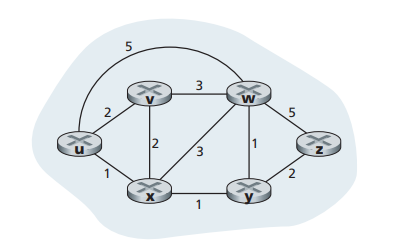
\includegraphics[width = 0.5\linewidth]{img/4/control-plane/state-link/graph-example.png}
    \caption{``Abstract graph model of a computer network''\cite{Kurose2017}}
    \label{fig:graph-example}
\end{figure}

\begin{figure}[H]
    \centering
    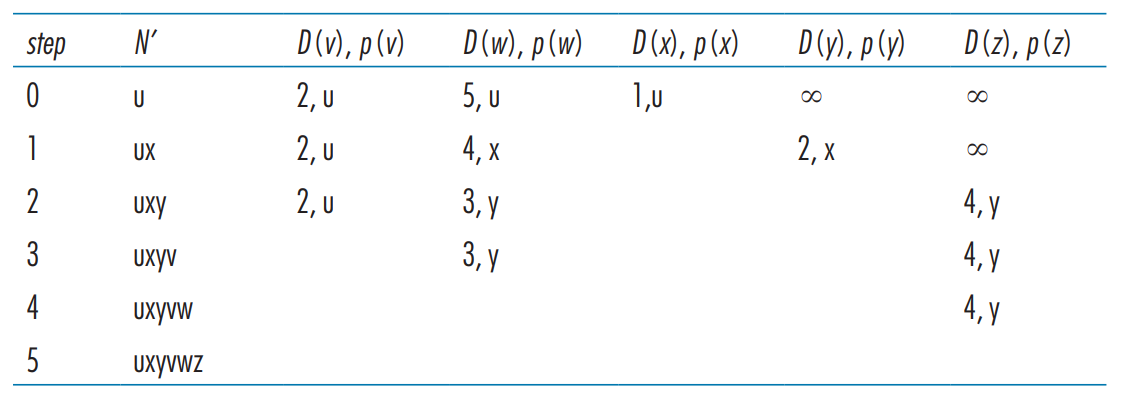
\includegraphics[width = 0.85\linewidth]{img/4/control-plane/state-link/dijkstra.png}
    \caption{``Running the link-state algorithm on the network''\cite{Kurose2017}}
    \label{fig:dijkstra}
\end{figure}

\begin{figure}[H]
    \centering
    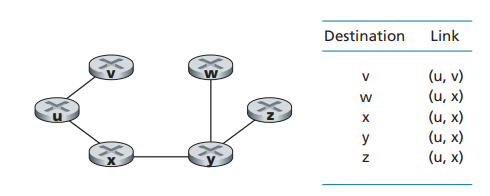
\includegraphics[width = 0.7\linewidth]{img/4/control-plane/state-link/shortest-path.png}
    \caption{``Least cost path and forwarding table for node \texttt{u}''\cite{Kurose2017}}
    \label{fig:shortest-path}
\end{figure}

%//==============================--@--==============================//%
\clearpage
\paragraph[4.3.1.2 Distance-Vector Protocols]{$\pmb{\star}$ Distance-Vector Protocols (decentralized routing algorithm)}\mbox{}

$$
    \text{\underline{Bellman-Ford equation:}} \quad \boxed{ D_\texttt{x}(\texttt{y}) = \min_\texttt{v}\{\, \text{c}(\texttt{x}, \texttt{v}) + D_\texttt{v}(\texttt{y})\, \} }
$$
Distance-vector protocols employ the Bellman-Ford algorithm to compute the shortest path. They involve:

\begin{itemize}
    \item \textbf{Routing table exchange:} Routers periodically exchange routing tables with neighbors, updating their tables accordingly.
    
    \item \textbf{Route selection:} Routers use the Bellman-Ford algorithm to update routing tables and determine the best path to each destination.
    
    \item \textbf{Count to infinity problem:} Slow convergence may lead to \underline{routing loops} and suboptimal paths. "Split horizon" and "poison reverse" techniques can mitigate this problem.
\end{itemize}

\definecolor{codegray}{rgb}{0.5, 0.5, 0.5}
\definecolor{codeblack}{rgb}{0.0, 0.0, 1.0}
\definecolor{codeorange}{rgb}{0.8, 0.33, 0.0}
\definecolor{codered}{rgb}{1.0, 0.03, 0.0}
\begin{lstlisting}[language=, title={``Distance-Vector (DV) Algorithm''\cite{Kurose2017}}, frame=tb, basicstyle=\scriptsize\ttfamily, escapechar=\%]
%\color{codeblack}initialization:%
    %\color{codeorange}for% all destinations y in N:
        %$\texttt{D}_\texttt{x}(\texttt{y})$% = c(x,y) %\color{codegray} /* if y is not a neighbor then c(x,y)= $+\infty$ */%
    %\color{codeorange}for% each neighbor w
        %$\texttt{D}_\texttt{w}(\texttt{y})$% = ? for all destinations y in N
    %\color{codeorange}for% each neighbor w
        %\color{codeorange}send% distance vector %$\texttt{D}_\texttt{x}$% = [%$\texttt{D}_\texttt{x}(\texttt{y})$%: y in N] to w

%\color{codeblack}loop% {
    %\color{codered}wait% %\color{codeorange}until% 
        I see a link cost change to some neighbor w
    %\color{codeorange}or until% 
        I receive a distance vector from some neighbor w
    
    %\color{codeorange}for% each y in N:
        %$\texttt{D}_\texttt{x}(\texttt{y})$% = min_v{c(x,v) + %$\texttt{D}_\texttt{v}(\texttt{y})$%}
    
    %\color{codeorange}if% %$\texttt{D}_\texttt{x}(\texttt{y})$% changed for any destination y
        %\color{codeorange}send% distance vector %$\texttt{D}_\texttt{x}$% = [%$\texttt{D}_\texttt{x}(\texttt{y})$%: y in N] to all neighbors
} %\color{codeblack}forever%
\end{lstlisting}

\vspace{1em}
\noindent \textbf{Addressing Routing Loops in Distance-Vector Protocols:}
\begin{itemize}
    \item \textbf{Routing loops} occur when a packet is forwarded in a continuous loop between routers, causing degraded network performance and packet loss. They often result from incorrect routing information due to slow convergence or the count-to-infinity issue in distance-vector protocols.

    \item The \textbf{count-to-infinity} issue arises when routers incrementally update their routing tables with outdated information, causing the routing metric to increase indefinitely. This can lead to suboptimal routing decisions and loops.
    
    \item \textbf{Split horizon} prevents routing loops by not propagating routing information learned from a neighbor back to that same neighbor, avoiding the spread of incorrect routing information.
    
    \item \textbf{Poison reverse} mitigates routing loops by advertising unreachable destinations with an infinite metric, informing neighbors not to use the advertising router as a path to the destination.
    
    \item Combining \textbf{split horizon} and \textbf{poison reverse} techniques can effectively prevent and resolve routing loops, leading to a more stable and efficient network.
\end{itemize}

\newpage
\noindent \textbf{Pros \& Cons:}
\begin{table}[H]
    \begin{tabularx}{\linewidth}{>{\parskip1ex}X@{\kern4\tabcolsep}>{\parskip1ex}X}
    \toprule
    \hfil\bfseries Pros
    &
    \hfil\bfseries Cons 
    \\\cmidrule(r{3\tabcolsep}){1-1}\cmidrule(l{-\tabcolsep}){2-2}
    
    %% separated by empty line or \par
    Lower computational requirements com- pared to link-state protocols.\par
    Simpler to configure and maintain.
    &
    
    %% separated by empty line or \par
    Slower convergence, $\mathcal{O}(N \cdot E)$, leading to temporary routing loops and suboptimal paths.\par
    Limited network visibility.\par
    May not scale well in large networks due to the periodic exchange of routing tables.
    \\\bottomrule
    \end{tabularx}
    \caption{Pros \& cons: Distance-Vector Protocols.}
\end{table}

\noindent \textbf{Exemplo de execução do Distance-Vector algorithm:}
\begin{figure}[H]
    \centering
    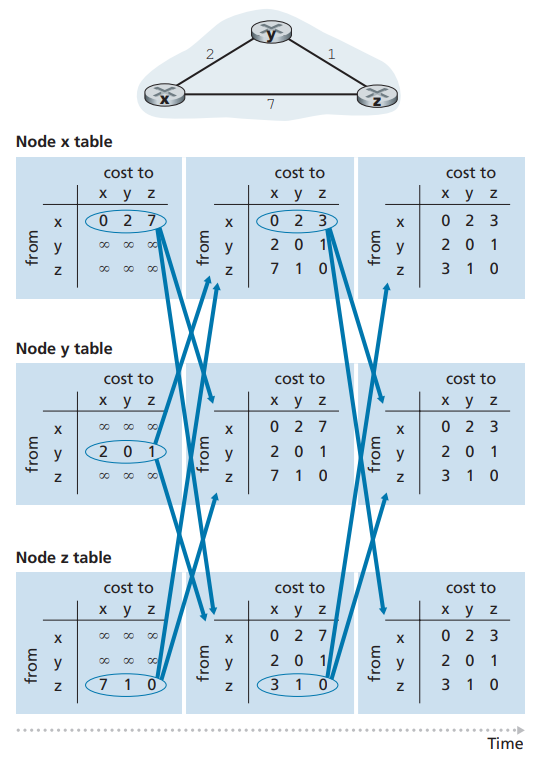
\includegraphics[width = 0.75\linewidth]{img/4/control-plane/distance-vector/DV-example.png}
    \caption{``Distance-vector (DV) algorithm in operation''\cite{Kurose2017}}
    \label{fig:shortest-path-DV}
\end{figure}

%//==============================--@--==============================//%
\clearpage
\paragraph[4.3.1.3 Path-Vector Protocols]{$\pmb{\star}$ Path-Vector Protocols}\mbox{}\\[4pt]
Path-vector routing protocols extend distance-vector protocols by sharing the entire path information to a destination. They involve:

\begin{itemize}
    \item \textbf{Path advertisement:} Routers advertise the entire path to each destination, instead of just the distance.
    
    \item \textbf{Path selection:} Routers use advertised paths to select the best path to each destination based on criteria such as path length, reliability, or administrative preferences.
    
    \item \textbf{Preventing routing loops:} Routers detect and prevent routing loops by checking for their own presence in the advertised path.
\end{itemize}

\vspace{1em}
\noindent \textbf{Pros \& Cons:}
\begin{table}[H]
    \begin{tabularx}{\linewidth}{>{\parskip1ex}X@{\kern4\tabcolsep}>{\parskip1ex}X}
    \toprule
    \hfil\bfseries Pros
    &
    \hfil\bfseries Cons 
    \\\cmidrule(r{3\tabcolsep}){1-1}\cmidrule(l{-\tabcolsep}){2-2}
    
    %% separated by empty line or \par
    More accurate and reliable path selection compared to distance-vector protocols.\par
    Prevents routing loops by detecting and discarding paths containing the router's own ID.\par
    Supports policy-based routing by allowing administrators to define routing preferences.
    &
    
    %% separated by empty line or \par
    Path advertisement can increase message size and bandwidth consumption.\par
    Requires more memory and processing power than distance-vector protocols, but less than link-state protocols.\par
    Less straightforward than distance-vector protocols in terms of configuration and troubleshooting.
    \\\bottomrule
    \end{tabularx}
    \caption{Pros \& cons: Path-Vector Protocols.}
\end{table}

%//==============================--@--==============================//%
\subsubsection[4.3.2 Hierarchical Routing and Autonomous Systems]{$\rightarrow$ Hierarchical Routing and Autonomous Systems}
\label{subsec:hierarchical-routing-autonomous-systems}

Hierarchical routing simplifies large-scale network routing by organizing the topology into hierarchical levels, reducing routing information, and improving scalability and convergence times.

\begin{itemize}
    \item \textbf{Autonomous Systems (ASes):} Collections of IP networks and routers controlled by a single organization with a common routing policy. The Internet is divided into thousands of ASes, each with a unique AS number.
    
    \item \textbf{Levels:} Hierarchical routing divides networks into tiers, such as core and edge, or additional levels like regional or local tiers.
    
    \item \textbf{Addressing:} Each hierarchy level has a unique address space, enabling efficient address aggregation and route summarization.
    
    \item \textbf{Route Aggregation and Summarization:} Higher-level routers maintain summarized routes, reducing the number of routes to store and exchange, and conserving resources.
    
    \item \textbf{Isolation:} Hierarchical routing isolates failures and updates within specific hierarchy levels or ASes, preventing network-wide instability.
\end{itemize}

\noindent Hierarchical routing is employed in both intradomain and interdomain routing, with OSPF and BGP using area or AS hierarchies. Intradomain routing within an AS uses protocols like OSPF, while interdomain routing between ASes is achieved through BGP.

%//==============================--@--==============================//%
\subsubsection[4.3.2 Intra-AS Routing in the Internet]{$\rightarrow$ Intra-AS Routing in the Internet}
\label{subsubsec:AS-protocols}

%//==============================--@--==============================//%
\paragraph[4.3.2.1 RIP: Routing Information Protocol]{$\pmb{\star}$ RIP: Routing Information Protocol}\mbox{}\\[4pt]
RIP is a distance-vector routing protocol that uses hop count as the metric for selecting the best path. It has a maximum hop count limit of 15, which restricts its scalability. Operates on top of UDP.

\begin{itemize}
    \item \textbf{RIP Inner Workings}: RIP routers exchange their routing tables every 30 seconds. Upon receiving an update, a router will compare the received routes with its own routing table and update its entries if a shorter path is found.
\end{itemize}

%//==============================--@--==============================//%
\paragraph[4.3.2.2 OSPF: Open Shortest Path First]{$\pmb{\star}$ OSPF: Open Shortest Path First}\mbox{}\\[4pt]
OSPF is a link-state routing protocol that calculates the shortest path using Dijkstra's algorithm. It is hierarchical and supports areas, allowing for better scalability compared to RIP.

\begin{itemize}
    \item OSPF is a widely used, open, link-state routing protocol for intra-AS routing.
    \item Routers construct a complete topological map of the AS and use Dijkstra's algorithm to determine shortest-path trees.
    \item Link costs can be configured by the network administrator, OSPF does not dictate how they are set.
    \item Routers broadcast routing information to all routers in the AS, not just their neighbors.
    \item Link-state information is broadcasted when a link's state changes or at least once every 30 minutes for robustness.
    \item \underline{OSPF messages are carried by IP} with an upper-layer protocol number of 89.
    \item The OSPF protocol implements functionality for reliable message transfer, link-state broadcast, link health check, and database synchronization with neighbors.
\end{itemize}

\noindent OSPF provides:

\begin{itemize}
    \item \textbf{Security:} OSPF supports authentication (simple and MD5) to prevent unauthorized routers from injecting incorrect information.
    \item \textbf{Multiple same-cost paths:} OSPF allows load balancing over multiple equal-cost paths.
    \item \textbf{Integrated support for unicast and multicast routing:} Multicast OSPF (MOSPF) extends OSPF to support multicast routing.
    \item \textbf{Support for hierarchy within a single AS:}
    \begin{itemize}[noitemsep, nolistsep]
        \item OSPF AS can be divided into areas, each running its own link-state routing algorithm.
        \item Area border routers handle routing between areas.
        \item One OSPF area is designated as the backbone area, which routes traffic between other areas.
    \end{itemize}
\end{itemize}

%//==============================--@--==============================//%
\clearpage
\subsubsection[4.3.3 Inter-AS Routing in the Internet]{$\rightarrow$ Inter-AS Routing in the Internet}
\label{subsubsec:inter-as}

%//==============================--@--==============================//%
\paragraph[4.3.3.1 BGP: Border Gateway Protocol]{$\pmb{\star}$ BGP: Border Gateway Protocol}\mbox{}\\[4pt]
BGP is a path-vector routing protocol designed for inter-domain routing between Autonomous Systems (ASes). It is crucial for the global Internet routing infrastructure.

\vspace{1 em}
\noindent BGP provides each router a means to:
\begin{itemize}
    \item Obtain prefix reachability information from neighboring ASes (allows each subnet to advertise its existence).
    \item Determine the “best” routes to the prefixes.
\end{itemize}

\noindent\textbf{Advertising BGP Route Information:} BGP routers, also known as "peers" or "neighbors," exchange routing updates containing the entire AS-path information. BGP uses various attributes, such as AS-path length and local preference, to select the best path.

\begin{itemize}
    \item \textbf{eBGP:} External BGP is used to exchange routing information between ASes.
    \item \textbf{iBGP:} Internal BGP is used to exchange routing information within the same AS.
\end{itemize}

\vspace{-1.0 em}
\begin{figure}[H]
    \centering
    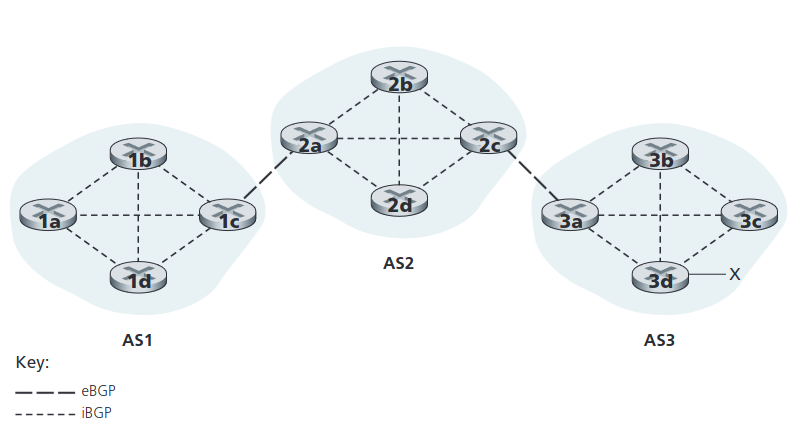
\includegraphics[width = 0.825\linewidth]{img/4/control-plane/BGP/BGP.png}
    \caption{eBGP and iBGP connections. Notice that iBGP connections do not necessarily follow the physical link between routers, in order to propagate the reachability information, both iBGP and eBGP sessions are used.}
    \label{fig:BGP}
\end{figure}

\renewcommand*{\thefootnote}{\fnsymbol{footnote}}
\footnotetext[4]{%
    \noindent\textbf{Commercial Routing Between Autonomous Systems} \mbox{}
    
    \noindent In the context of commercial routing, ASes can establish various types of relationships, such as transit, peering, or customer-provider relationships. These relationships dictate how routing information is exchanged and propagated through the Internet.
    
    \begin{itemize}
        \item \textbf{Transit:} A transit AS provides connectivity for other ASes to reach the global Internet. Transit providers typically charge for their services.
        
        \item \textbf{Peering:} In a peering relationship, two ASes agree to exchange routing information without charging each other. This is commonly established between ISPs of similar size for mutual benefit.
        
        \item \textbf{Customer-Provider:} In this relationship, a provider AS offers Internet access and routing services to a customer AS. The customer typically pays the provider for the services.
    \end{itemize}
}
\renewcommand*{\thefootnote}{\arabic{footnote}}

\newpage
\noindent\textbf{Route Selection in BGP}\mbox{}

\noindent Determining the Best Routes in BGP involves considering multiple paths from a given router to a destination subnet. BGP routers often receive reachability information about dozens of different possible paths. A router chooses among these paths and configures its forwarding table accordingly. When a router advertises a prefix across a BGP connection, it includes several BGP attributes, such as \texttt{AS-PATH} and \texttt{NEXT-HOP}, with the prefix.

\begin{itemize}
    \item \textbf{AS-PATH} contains the list of ASes traversed by the advertisement. Routers use the \texttt{AS-PATH} attribute to detect and prevent looping advertisements by rejecting advertisements containing their own AS in the path list. 

    \item \textbf{NEXT-HOP} is the IP address of the router interface that begins the \texttt{AS-PATH}. It serves as the critical link between inter-AS and intra-AS routing protocols.

    \item \textbf{LOCAL-PREF} is a BGP attribute representing the local preference value assigned to a route within an AS. This value is not passed outside the AS and is used to select the preferred exit point from the AS for a given route. The higher the local preference value, the more preferred the route.

    \item \textbf{MED} (Multi-Exit Discriminator) is another BGP attribute used to influence the choice of entry point to an AS for incoming traffic. The \texttt{MED} value suggests the preferred entry point by comparing the \texttt{MED} values of different routes advertised by neighboring ASes. The lower the \texttt{MED} value, the more preferred the route.
\end{itemize}

\begin{figure}[H]
    \centering
    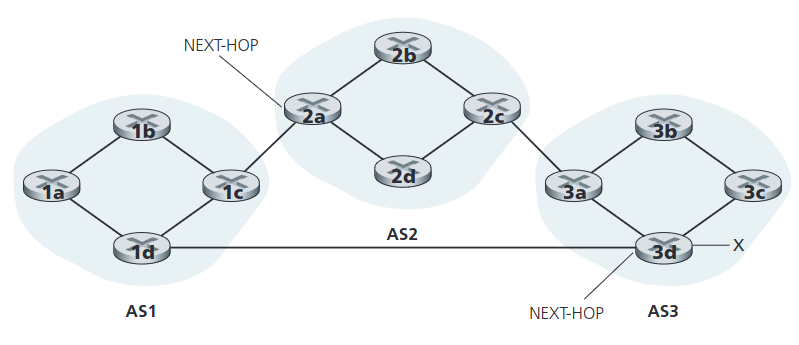
\includegraphics[width = 0.825\linewidth]{img/4/control-plane/BGP/route.png}
    \caption{The IP address of the leftmost interface of router 3d and of router 2a are known as Next-Hop.}
    \label{fig:route}
\end{figure}

\noindent\textbf{Hot Potato Routing Algorithm}\mbox{}

\noindent Hot potato routing, also known as "early-exit" or "closest-exit" routing, is a strategy used to select the best path based on the shortest internal distance within an AS. Hot potato is a selfish algorithm: it tries to reduce the cost in its own AS while ignoring the other components of the end-to-end costs outside its AS.

\begin{figure}[H]
    \centering
    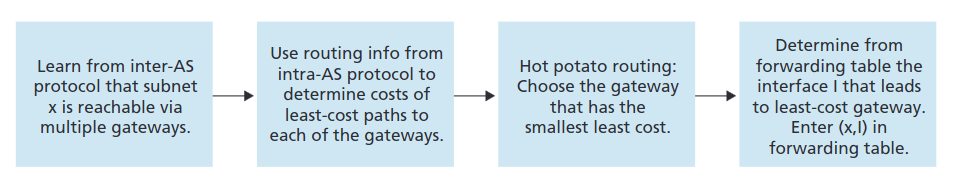
\includegraphics[width = 0.85\linewidth]{img/4/control-plane/BGP/hot-potato.png}
    \caption{Hot potato algorithm \cite{Kurose2017}}
    \label{fig:Hot-potato}
\end{figure}

\noindent\textbf{BGP Route-Selection Algorithm}\mbox{}

\noindent In practice, BGP uses a more sophisticated route-selection algorithm that incorporates Hot Potato Routing and takes \texttt{LOCAL-PREF} and \texttt{MED} into account. For any given destination prefix, the input into BGP's route-selection algorithm is the set of all routes to that prefix that have been learned and accepted by the router. BGP sequentially invokes the following elimination rules until one route remains:

\begin{enumerate}
    \item Select the routes with the highest local preference values (\texttt{LOCAL-PREF}).
    \item From the remaining routes, select the route with the shortest \texttt{AS-PATH}.
    \item From the remaining routes, choose the route with the lowest \texttt{MED} value.
    \item From the remaining routes, use Hot Potato Routing to select the route with the closest \texttt{NEXT-HOP} router.
    \item If more than one route still remains, use other BGP identifiers to select the route.
\end{enumerate}

\noindent\textbf{Route Filtering and Policy Control in BGP}\mbox{}

\noindent BGP provides various methods for filtering and controlling route advertisements to implement routing policies.

\begin{itemize}
    \item \textbf{Prefix Lists:} Used to filter routes based on the IP prefix.
    
    \item \textbf{AS-PATH Access Lists:} Used to filter routes based on the \texttt{AS-PATH} attribute.
    
    \item \textbf{Route Maps:} Used to apply complex policies that involve multiple BGP attributes. Route maps can manipulate attributes or filter routes based on various criteria.

    \item Each AS may choose to \underline{not} advertise their routes to neighbouring ASes.

    \item Each AS attributes a preference value to the routes advertised by their neighbors.
\end{itemize}

\noindent By utilizing these filtering and policy control methods, BGP allows network administrators to manage inter-domain routing and implement policies based on commercial agreements or traffic engineering requirements.

\begin{itemize}
    \item \textbf{AS routing policy can trump other considerations}, such as shortest AS path or hot potato routing; local-preference attribute value is fixed by the policy of the local AS.
    
    \item \underline{Access ISP\footnotemark[4] networks (last-mile/local ISPs)} \textbf{advertise no paths to any other destinations except themselves}, ensuring all traffic leaving/entering them must have the source/destination within their own network.

    \item The rule of thumb followed by commercial ISPs: \textbf{any traffic flowing across an ISP's backbone network must have either a source or a destination (or both) in a network that is a \underline{customer of that ISP}}.
    
    \item Differences between inter-AS and intra-AS routing protocols: Policy (dominates in inter-AS routing), Scale (critical for inter-AS routing, less so for intra-AS routing), and Performance (less important in inter-AS routing due to policy constraints).
\end{itemize}

\footnotetext[4]{%
    Access ISPs are usually connected to higher-tier ISPs, such as Tier-1 or Tier-2 ISPs, which have broader network coverage and provide backbone connectivity for lower-tier ISPs. In this sense, access ISPs are at the bottom of the ISP hierarchy, as they primarily focus on providing Internet services directly to the end-users.
}

%//==============================--@--==============================//%

        \clearpage
%//==============================--@--==============================//%
\subsection[4.4 Data Plane]{\hspace*{0.075 em}\raisebox{0.2 em}{$\pmb{\drsh}$} Data Plane}
\label{subsec:data-plane}

%//==============================--@--==============================//%
\subsubsection[4.4.1 IPv4 Datagram Format]{$\rightarrow$ IPv4 Datagram Format}

\vspace{-0.5em}
\begin{figure}[H]
    \centering
    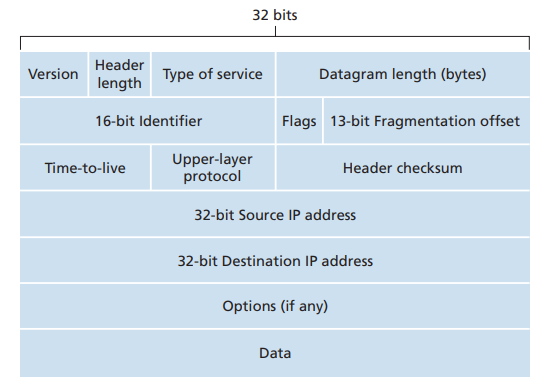
\includegraphics[width = 0.7\linewidth]{img/4/data-plane/IPv4-datagram-format.png}
    \caption{IPv4 Datagram format \cite{Kurose2017}}
    \label{fig:IPv4}
\end{figure}

\begin{itemize}
    \item \textbf{Version number (4 bits):} Specifies the IP protocol version of the datagram, e.g., IPv4 or IPv6.
    
    \item \textbf{Header length (4 bits):} Indicates where the payload begins, considering variable number of options in the header.
    
    \item \textbf{Type of service (8 bits):} Distinguishes different types of IP datagrams, e.g., real-time vs non-real-time traffic, and supports Explicit Congestion Notification.
    
    \item \textbf{Datagram length (16 bits):} Total length of the IP datagram (header plus data) in bytes, with a theoretical maximum size of 65,535 bytes.
    
    \item \textbf{Identifier, flags, fragmentation offset (32 bits):} Related to IP fragmentation, where large datagrams are split into smaller ones, then reassembled at the destination.
    
    \item \textbf{Time-to-live (8 bits):} Ensures datagrams don't circulate indefinitely; decre- mented by one at each router, and dropped when reaching zero.
    
    \item \textbf{Protocol (8 bits):} Indicates the transport-layer protocol for the payload (e.g., 6 for TCP, 17 for UDP).
    
    \item \textbf{Header checksum (16 bits):} Helps detect bit errors in the received IP datagram using 1s complement arithmetic; recomputed and stored at each router.
    
    \item \textbf{Source IP address (32 bits):} IP address of the sender.
    
    \item \textbf{Destination IP address (32 bits):} IP address of the intended recipient.
    
    \item \textbf{Options (variable):} Allow IP header to be extended; used rarely and not included in IPv6 header.
    
    \item \textbf{Data (payload):} Contains the transport-layer segment (e.g., TCP or UDP) or other data types (e.g., ICMP messages) to be delivered to the destination.
\end{itemize}

%//==============================--@--==============================//%
\subsubsection[4.4.2 IPv4 Addressing]{$\rightarrow$ IPv4 Addressing}

\noindent Each IP address is 32 bits long (equivalently, 4 bytes). These addresses are typically written in so-called dotted-decimal notation, in which each byte of the address is written in its decimal form and is separated by a period (dot) from other bytes in the address:
$$
    \texttt{193.32.216.9} \pmb{\rightarrow} \texttt{11000001 00100000 11011000 00001001}
$$

\paragraph[4.4.2.1 Subnet and CIDR]{$\pmb{\star}$ Subnet and CIDR}\mbox{}
\begin{theo}[\underline{Subnet}]{def:Subnet}\label{def:Subnet}
    ``To determine the subnets, detach each interface from its host or router, creating islands of isolated networks, with interfaces terminating the end points of the isolated networks. Each of these isolated networks is called a subnet."\cite{Kurose2017}
\end{theo}

\vspace{-0.5em}
\begin{figure}[H]
    \centering
    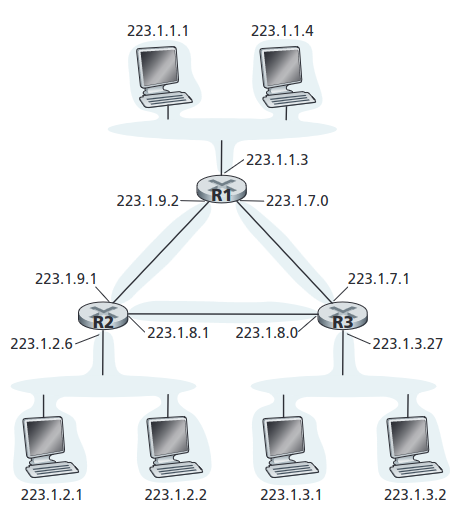
\includegraphics[width = 0.5\linewidth]{img/4/data-plane/Subnets}
    \caption{3 routers connected to 6 subnets}
    \label{fig:Subnet}
\end{figure}

\begin{itemize}[noitemsep, nolistsep]
    \item The boundary between the host and the physical link is called an \textbf{interface}. A router may have more than one interface (In \hyperref[fig:Subnet]{Fig. 39} each of the three routers possess 3 different interfaces)
    
    \item Multiple subnets can exist in a network, including point-to-point links connecting routers (see \hyperref[fig:Subnet]{Fig. 39}).
    
    \item An organization's network devices typically have IP addresses with a common network prefix.
    
    \item \textbf{Classless Interdomain Routing (CIDR)} generalizes subnet addressing by dividing the 32-bit IP address into two parts, with the network prefix indicated by x (\textbf{subnet mask}) in the a.b.c.d/x format (e.g.: \texttt{223.3.2.1/24} has prefix \texttt{223.3.2}).

    \item The x most significant bits are the network prefix, while the remaining 32-x bits can be used for subnetting within the organization.
\end{itemize}

\vspace{1 em}
\noindent\textbf{Nota:}\\
Address \texttt{255.255.255.255} is known has a brodcast address and is used to deliver a message to all hosts in the same subnet.

\paragraph[4.4.2.2 Allocating a block of addresses ]{$\pmb{\star}$ Allocating a block of addresses}\mbox{}
\begin{itemize}
    \item Network administrators obtain IP address blocks for their organizations from ISPs.
    
    \item ISPs can divide a larger allocated block into smaller blocks for their customers (e.g.: ISP's block \texttt{200.23.16.0/20} can be divided into eight smaller blocks for organizations such as \texttt{200.23.16.0/23}, \texttt{200.23.18.0/23} and so on).
    
    \item ISPs and other organizations can also obtain IP address blocks from a global authority, the \textbf{Internet Corporation for Assigned Names and Numbers (ICANN)}.
    
    \item ICANN manages IP addresses, DNS root servers, domain names, and domain name disputes, and allocates addresses to regional Internet registries.
\end{itemize}

%//==============================--@--==============================//%
\subsubsection[4.4.3 The Dynamic Host Configuration Protocol (DHCP)]{$\rightarrow$ The Dynamic Host Configuration Protocol (DHCP)}

\begin{itemize}
    \item Dynamic Host Configuration Protocol (DHCP) automates IP address assignment for hosts.
    \item Provides plug-and-play or zero-configuration functionality.
    \item Widely used in residential, enterprise, and wireless networks.
    \item DHCP operates as a client-server protocol.
    \item If no server is present on a subnet, a DHCP relay agent (typically a router) is needed.
\end{itemize}

\begin{figure}[H]
    \centering
    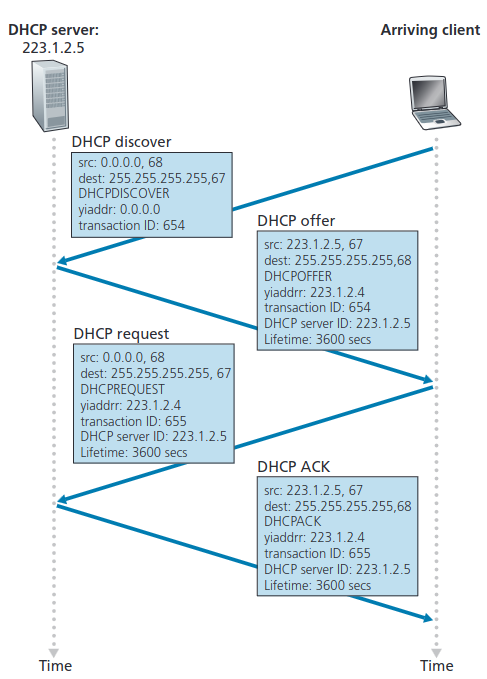
\includegraphics[width = 0.6\linewidth]{img/4/data-plane/DHCP.png}
    \caption{Client-server DHCP protocol}
    \label{fig:DHCP}
    \end{figure}

\begin{enumerate}[nolistsep]
    \item \textbf{DHCP server discovery:} Client sends a DHCP discover message using the broadcast destination IP address \texttt{255.255.255.255} and source IP address \texttt{0.0.0.0.}
    
    \item \textbf{DHCP server offer(s):} DHCP server responds with a DHCP offer message, also broadcast to all nodes on the subnet. Offer message contains transaction ID, proposed IP address, network mask, and IP address lease time.
    
    \item \textbf{DHCP request:} Client chooses an offer and responds with a DHCP request message, echoing back the configuration parameters (usually DHCP request is broadcasted, however, the client can choose to unicast it directly to the DHCP server if the server's IP address is known, the same can be said for DHCP ACK).
    
    \item \textbf{DHCP ACK:} Server responds with a DHCP ACK message, confirming the requested parameters.
\end{enumerate}

%//==============================--@--==============================//%
\subsubsection[4.4.4 Network Address Translation (NAT)]{$\rightarrow$ Network Address Translation (NAT)}

\begin{figure}[H]
    \centering
    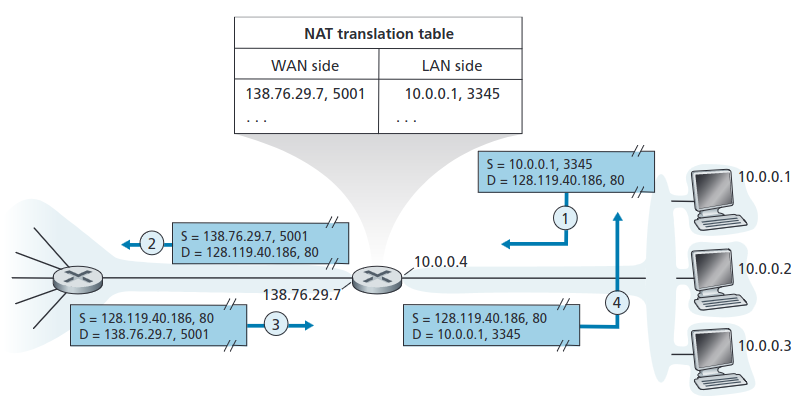
\includegraphics[width = 0.9\linewidth]{img/4/data-plane/NAT.png}
    \caption{Network address translation}
    \label{fig:NAT}
\end{figure}

\noindent The NAT-enabled router does not look like a router to the outside world. Instead
the NAT router behaves to the outside world as a single device with a single IP
address, possessing a \textbf{NAT translation table} capable of redirecting any messages to their specified destination through an (IP, PORT) association:

\begin{enumerate}
    \item User requests a Web page from a Web server (port 80) with IP address \texttt{128.119.40.186}.
    \item Host \texttt{10.0.0.1} assigns source port number 3345 and sends the datagram into the LAN.
    \item NAT router generates a new source port number 5001, replaces the source IP address and port, and adds an entry to its NAT translation table.
    \item Web server responds with a datagram \textbf{whose destination address is the NAT router's IP address}, and \textbf{destination port number is 5001}.
    \item NAT router uses the NAT translation table to obtain the appropriate IP address and destination port number for the browser in the home network, rewrites the datagram's destination address and port, and forwards the datagram into the home network.
\end{enumerate}

%//==============================--@--==============================//%
\clearpage
\subsubsection[4.4.5 IPv6 Datagram Format]{$\rightarrow$ IPv6 Datagram Format}

In the early 1990s, the Internet Engineering Task Force (IETF) began developing a successor to the IPv4 protocol due to concerns that the 32-bit IPv4 address space was running out. This led to the creation of the IPv6 protocol, which aimed to address the limitations of IPv4 and introduce improvements based on accumulated operational experience.

\begin{mdframed}
    \begin{itemize}[nolistsep, noitemsep]
        \item \textbf{IPv6 Address Representation:}
        \begin{itemize}[nolistsep, noitemsep]
            \item IPv6 addresses are 128 bits long, separated into 8 fields of 16 bits each.
            \item Each 16-bit field is represented by 4 hexadecimal characters.
        \end{itemize}
        \item Example:
        \begin{itemize}[nolistsep, noitemsep]
            \item Original: \texttt{2001:0db8:130f:0000:0000:7000:0000:140b}
            \item Simplified (without leading zeros): \texttt{2001:db8:130f:0:0:7000:0:140b}
            \item Further simplified (with consecutive zero fields replaced by "\texttt{::}"): \texttt{2001:db8:130f::7000:0:140b}
        \end{itemize}
    \end{itemize}
\end{mdframed}

\vspace{-0.5em}
\begin{figure}[H]
    \centering
    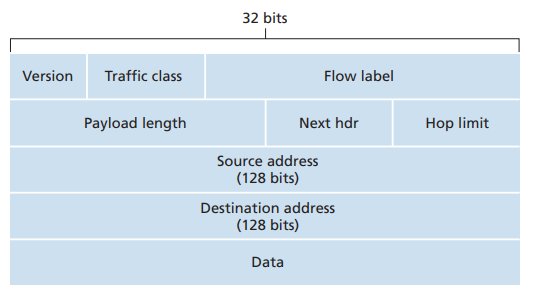
\includegraphics[width = 0.7\linewidth]{img/4/data-plane/IPv6-datagram-format.png}
    \caption{IPv6 Datagram format \cite{Kurose2017}}
    \label{fig:IPv6}
\end{figure}

\begin{itemize}
    \item \textbf{Version (4 bits):} Identifies the IP version number; IPv6 carries a value of 6.
    
    \item \textbf{Traffic class (8 bits):} Prioritizes certain datagrams within a flow or from specific applications, similar to the Type of Service in IPv4.
    
    \item \textbf{Flow label (20 bits):} Used to identify a flow of datagrams, with an elusive definition; could distinguish traffic from different applications or users.
    
    \item \textbf{Payload length (16 bits):} Unsigned integer giving the number of bytes in the IPv6 datagram following the fixed-length, 40-byte datagram header.
    
    \item \textbf{Next header (8 bits):} Identifies the protocol to which the data field of the datagram will be delivered (e.g., TCP, UDP); same values as IPv4 protocol field.
    
    \item \textbf{Hop limit (8 bits):} Contents decremented by one at each router; if the count reaches zero, the router discards the datagram.
    
    \item \textbf{Source address (128 bits):} IPv6 address of the sender, described in RFC 4291.
    
    \item \textbf{Destination address (128 bits):} IPv6 address of the intended recipient, described in RFC 4291.
    
    \item \textbf{Data (payload):} Transport-layer segment (e.g., TCP, UDP) or other data types (e.g., ICMP messages) to be delivered to the destination.
\end{itemize}

\noindent IPv6 also omits certain fields that were present in the IPv4 datagram format:
\begin{itemize}
    \item \textbf{Fragmentation/reassembly:} IPv6 does not allow fragmentation and reassembly at intermediate routers. If an IPv6 datagram is too large to be forwarded, the router drops the datagram and sends a "Packet Too Big" ICMP error message back to the sender, who can then resend the data using a smaller IP datagram size.

    \item \textbf{Header checksum:} Due to checksumming already being performed at the transport layer and link layer in the Internet, the header checksum was considered redundant and removed to speed up IP packet processing.

    \item \textbf{Options:} The options field is no longer a part of the standard IP header. Instead, it can be one of the possible next headers pointed to from within the IPv6 header, alongside TCP or UDP protocol headers. This change results in a fixed-length, 40-byte IP header.
\end{itemize}

\paragraph[4.4.5.1 Transitioning from IPv4 to IPv6]{$\pmb{\star}$ Transitioning from IPv4 to IPv6}\mbox{}

\begin{itemize}
    \item New IPv6 systems can be made backward-compatible, but deployed IPv4 systems cannot handle IPv6 datagrams.
    \item A "flag day" for simultaneous transition from IPv4 to IPv6 is not feasible due to the vast number of devices.
\end{itemize}

\begin{theo}[\underline{Tunneling}]{def:tunneling}\label{def:tunneling}
    \begin{itemize}[nolistsep,noitemsep]
        \item The most widely adopted approach for IPv4-to-IPv6 transition.
        \item IPv6 nodes wanting to communicate are connected by intervening IPv4 routers (forming a tunnel).
        \item The IPv6 node on the sending side encapsulates the entire IPv6 datagram into the payload field of an IPv4 datagram using the IPv6 protocol (number 41).
        \item The IPv4 routers in the tunnel route the IPv4 datagram without knowing it contains an IPv6 datagram, only aware of the IPv4 header information.
        \item The IPv6 node on the receiving side extracts the IPv6 datagram from the IPv4 datagram by recognizing protocol number 41 and routes it accordingly.
    \end{itemize}
\end{theo}

\begin{figure}[H]
    \centering
    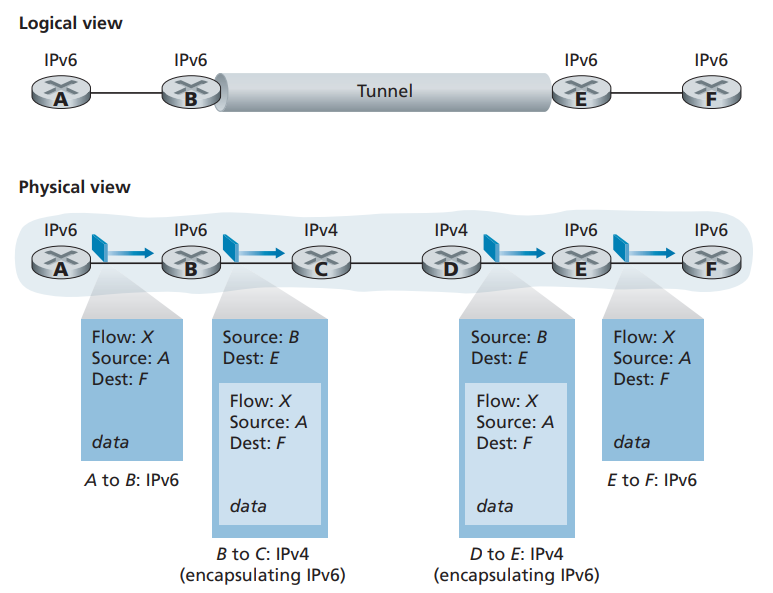
\includegraphics[width = 0.65\linewidth]{img/4/data-plane/tunneling.png}
    \caption{Tunneling \cite{Kurose2017}}
    \label{fig:tunneling}
\end{figure}

\newpage
\subsubsection[4.4.6 ICMP: The Internet Control Message Protocol]{$\rightarrow$ ICMP: The Internet Control Message Protocol}
\begin{theo}[\underline{ICMP}]{def:ICMP}\label{def:ICMP}
    ICMP is often considered part of IP, but architecturally it lies just above IP, as ICMP messages are carried inside IP datagrams. That is, ICMP messages are carried as IP payload, just as TCP or UDP segments are carried as IP payload. Similarly, when a host receives an IP datagram with ICMP specified as the upper-layer protocol (an upper-layer protocol number of 1), it demultiplexes the datagram’s contents to ICMP, just as it would demultiplex a datagram’s content to TCP or UDP.
\end{theo}

\noindent ICMP messages consist of \textbf{type} and \textbf{code fields} and contains the \textbf{header of first 8 bytes of the triggering IP datagram}. ICMP messages are not only for error signaling; the ping program sends an ICMP echo request and the destination host responds with an ICMP echo reply. Traceroute is implemented with ICMP messages, sending a series of IP datagrams with increasing TTL values to identify routers and round-trip times between the source and destination hosts. ICMPv6 has reorganized the existing ICMP types and codes and added new ones for IPv6 functionality.

\begin{figure}[H]
    \centering
    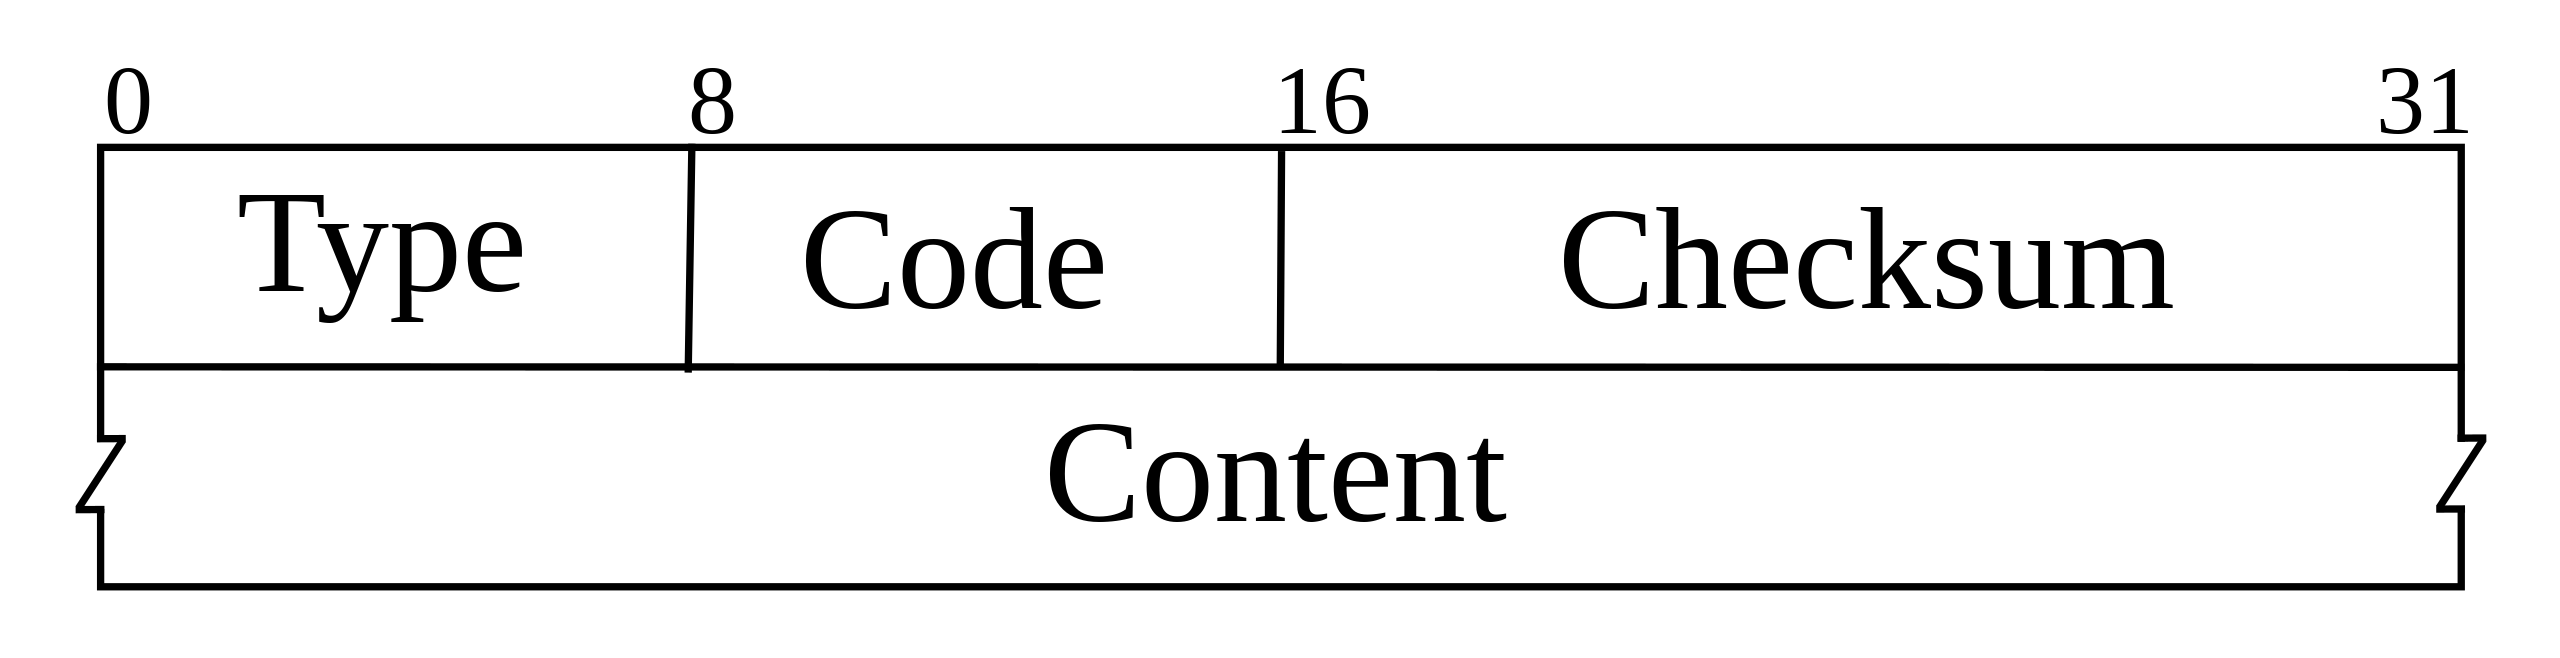
\includegraphics[width = 0.65\linewidth]{img/4/data-plane/ICMP-segment.png}
    \caption{ICMP header}
    \label{fig:icmp-header}
\end{figure}

{
\setlength{\tabcolsep}{32pt}

\begin{table}[h!]
    \centering
    \captionsetup{justification=centering}
    \begin{tabularx}{\textwidth}{ccl}
        \toprule
        \textbf{ICMP Type} & \textbf{Code} & \multicolumn{1}{c}{\textbf{Description}} \\
        \midrule
        0 & 0 & Echo reply (to ping) \\
        3 & 0 & Destination network unreachable \\
        3 & 1 & Destination host unreachable \\
        3 & 2 & Destination protocol unreachable \\
        3 & 3 & Destination port unreachable \\
        3 & 6 & Destination network unknown \\
        3 & 7 & Destination host unknown \\
        4 & 0 & Source quench (congestion control) \\
        5 & 0 & Redirect Datagram for the Network \\
        5 & 1 & Redirect Datagram for the Host \\
        5 & 2 & \>\> for the Type of Service and Network \\
        5 & 3 & \>\> for the Type of Service and Host \\
        8 & 0 & Echo request \\
        9 & 0 & Router advertisement \\
       10 & 0 & Router discovery \\
       11 & 0 & TTL expired \\
       12 & 0 & IP header bad \\
        \bottomrule
    \end{tabularx}
    \caption{ICMP message types \cite{Kurose2017}}
    \label{tab:icmp}
\end{table}
}

\clearpage
\noindent ICMP redirects (types 5, codes 0-3) are used by routers to inform the sender that there is a more optimal route to the destination. When a router receives a packet and determines that the packet's next hop should be on the same interface it was received, the router sends an ICMP redirect message to the sender, indicating a more direct route to the destination. This can help optimize network traffic and reduce unnecessary load on routers.

\vspace{1 em}
\noindent Here's an example scenario:
\begin{enumerate}
    \item Host A wants to send a packet to Host B.
    \item Host A's routing table indicates that it should send the packet to Router 1.
    \item Router 1 receives the packet, but based on its routing table, it determines that Host A should have sent the packet directly to Host B or to another router, Router 2, on the same network segment instead.
    \item Router 1 sends an ICMP redirect message to Host A, notifying it that there is a more optimal route available to reach Host B.
    \item Host A updates its routing table based on the received ICMP redirect message and sends subsequent packets to Host B using the new, more optimal route.
\end{enumerate}

\noindent This process allows the network to self-optimize and avoid sending packets through unnecessary or suboptimal paths. However, it's worth mentioning that ICMP redirects are sometimes disabled for security reasons, as they can be exploited for man-in-the-middle attacks.

\vspace{1 em}
\begin{figure}[H]
    \centering
    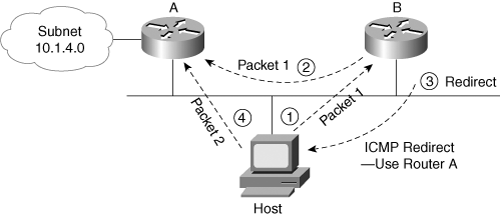
\includegraphics[width = 0.8\linewidth]{img/4/data-plane/ICMP-redirect.png}
    \caption{ICMP redirect}
    \label{fig:icmp-redirect}
\end{figure}

%//==============================--@--==============================//%

    \clearpage\addtocontents{toc}{\protect\newpage}
    \section{5. Camada de Ligação de Dados}\label{sec:link-layer}%
        %//==============================--@--==============================//%
\subsection[5.1 Visão Geral]{\hspace*{0.075 em}\raisebox{0.2 em}{$\pmb{\drsh}$} Visão Geral}
\label{subsec:visao-geral}

\begin{theo}[\underline{Link Layer}]{def:Link-Layer}\label{def:Link-Layer}
    ``The basic service of any link layer is to move a datagram from one node to an adjacent node over a single communication link."\cite{Kurose2017}
\end{theo}

\noindent The link layer may provide the following services:
\begin{itemize}
    \item \textbf{Framing:} Encapsulates network-layer datagrams in link-layer frames. A frame consists of a data field, in which the network-layer datagram is inserted, and a number of header fields.
    \item \textbf{Link access:} MAC (Medium Access Control) protocol governs frame transmission, coordinating multiple nodes on a broadcast link.
    \item \textbf{Reliable delivery:} Ensures error-free transmission across the link, useful for high-error-rate links but unnecessary for low-error-rate links.
    \item \textbf{Error detection and correction:} Identifies and corrects bit errors introduced by signal attenuation and electromagnetic noise.
\end{itemize}

\noindent The link layer implementation:
\begin{itemize}
    \item Involves both hardware and software components.
    \item Uses a \textbf{network adapter}, also known as a \textbf{network interface controller (NIC)} for hardware implementation.
    \item Can be integrated into the motherboard chipset or implemented via a dedicated Ethernet chip.
    \item Handles various link layer services including framing, link access, and error detection.
\end{itemize}

\begin{figure}[H]
    \centering
    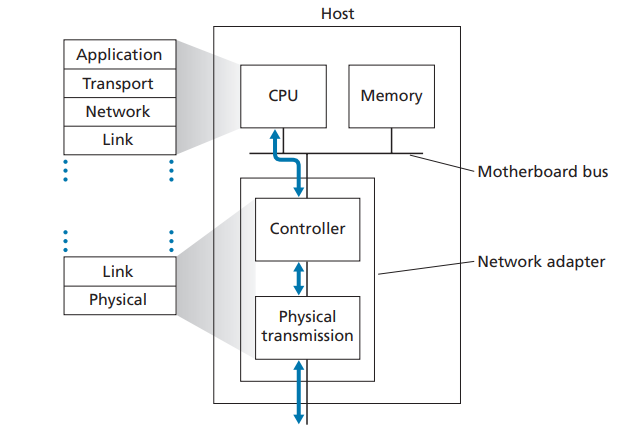
\includegraphics[width = 0.75\linewidth]{img/5/network-adapter.png}
    \caption{``Network adapter: relationship to other host components and to protocol stack functionality''\cite{Kurose2017}}
    \label{fig:network-adapter}
\end{figure}

\newpage
\noindent The link layer in the protocol stack involves both hardware and software components:
\begin{itemize}
    \item On the sending side:
    \begin{itemize}[nolistsep, noitemsep]
        \item The network adapter takes a datagram created and stored in host memory by higher layers of the protocol stack.
        \item It encapsulates the datagram in a link-layer frame.
        \item The frame is transmitted into the communication link following the link-access protocol.
    \end{itemize}
    \item On the receiving side:
    \begin{itemize}[nolistsep, noitemsep]
        \item The network adapter receives the entire frame.
        \item It extracts the network-layer datagram.
        \item Error detection is performed, if necessary.
    \end{itemize}
    \item Higher-level link-layer features are implemented in software running on the host's CPU:
    \begin{itemize}[nolistsep, noitemsep]
        \item Software components assemble link-layer addressing information.
        \item They activate the controller hardware.
        \item Error conditions are handled, and datagrams are passed up to the network layer.
    \end{itemize}
\end{itemize}

%//==============================--@--==============================//%
        %//==============================--@--==============================//%
\subsection[Link Layer Error-Detection and -Correction Techniques]{\hspace*{0.075 em}\raisebox{0.2 em}{$\pmb{\drsh}$} Link Layer Error-Detection and -Correction Techniques}
\label{subsec:link-layer-error-detection-correction}

Error-detection and -correction techniques in the link layer are essential for maintaining data integrity during transmission between physically connected neighboring nodes. These techniques detect and correct bit errors in the link-layer frame.

%//==============================--@--==============================//%
\subsubsection[Parity Checking]{$\pmb{\rightarrow}$ Parity Checking}

Parity checking is a basic error-detection technique that adds a single parity bit to the data being transmitted. The parity bit is set to make the total number of 1s in the data either even (even parity) or odd (odd parity). At the receiving end, the parity bit is checked to ensure that the total number of 1s is consistent with the selected parity scheme. If there is a discrepancy, an error is detected.

%//==============================--@--==============================//%
\subsubsection[Checksumming]{$\pmb{\rightarrow}$ Checksumming}

Checksumming is a more advanced error-detection technique that has been previously explained in the context of the \hyperref[subsubsec:checksum]{transport layer for UDP and TCP}. In this method, a checksum is calculated by the sender based on the data being transmitted and is then included with the transmitted data. At the receiving end, the receiver calculates the checksum based on the received data and compares it to the received checksum. If the calculated and received checksums do not match, an error is detected.

%//==============================--@--==============================//%
\subsubsection[Cyclic Redundancy Checks (CRC)]{$\pmb{\rightarrow}$ Cyclic Redundancy Checks (CRC)}

Cyclic Redundancy Check (CRC) is an error-detection technique widely used in computer networks. It works by interpreting the bit string as a polynomial and performing modulo-2 arithmetic operations. The sender calculates CRC bits (\texttt{R}) and appends them to the data (\texttt{D}) to create a bit pattern divisible by a generator (\texttt{G}). The receiver checks the received data for errors by dividing the received bit pattern by \texttt{G} and verifying if the remainder is zero.

\begin{figure}[H]
    \centering
    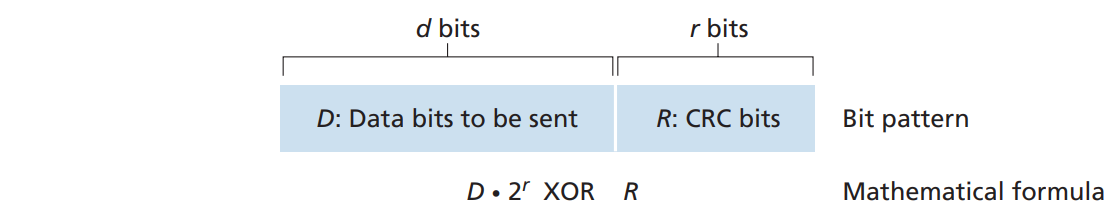
\includegraphics[width = 0.85\linewidth]{img/5/CRC.png}
    \caption{CRC (Cyclic Redundancy Check) \cite{Kurose2017}}
    \label{fig:CRC}
\end{figure}

\begin{enumerate}
    \item Choose a generator (\texttt{G}) with \texttt{r}+1 bits and make sure the leftmost bit of \texttt{G} is 1.
    \item Calculate the CRC bits (\texttt{R}) by finding the remainder of the division $\texttt{D} \cdot 2^\texttt{r}/\texttt{G}$, where \texttt{D} is the data bits.
    \item Append the CRC bits (\texttt{R}) to the data (\texttt{D}) and send the d+r bit pattern.
    \item The receiver divides the received $\texttt{d}+\texttt{r}$ bits by \texttt{G} using modulo-2 arithmetic.
    \item If the remainder is nonzero, an error has occurred; otherwise, the data is accepted as correct.
\end{enumerate}

\hrule

\begin{quote}
    \noindent ``International standards have been defined for 8-, 12-, 16-, and 32-bit generators (\texttt{G}). The CRC-32 32-bit standard, adopted in several link-level IEEE protocols, uses a generator:
    $$
        \texttt{G}_\text{ CRC-32} = \texttt{100000100110000010001110110110111}
    $$
    \noindent Each CRC standard can detect burst errors of fewer than $\texttt{r}+1$ bits, and under appropriate assumptions, a burst of length greater than $\texttt{r}+1$ bits is detected with a probability of $1 - 0.5^\texttt{r}$. Furthermore, each CRC standard can detect any odd number of bit errors.''\cite{Kurose2017}
\end{quote}

%//==============================--@--==============================//%

        %//==============================--@--===========================
\subsubsection[5.3 Multiple Access Links and Protocols]{\hspace*{0.075 em}\raisebox{0.2 em}{$\pmb{\drsh}$} Multiple Access Links and Protocols}

Broadcast links allow multiple nodes to send and receive data on a shared channel. Multiple access protocols coordinate transmissions to minimize collisions and optimize throughput; they widely used in various network settings such as wired and wireless access networks, satellite networks, and local area networks (LANs).  The three main categories of these protocols are channel partitioning, random access, and taking-turns protocols.

\vspace{1em}
\noindent An ideal multiple access protocol should have the following characteristics:
\begin{enumerate}
    \item When only one node has data to send, that node has a throughput of $R$ bps.
    \item When M nodes have data to send, each of these nodes has a throughput of $R/M$ bps. This implies that each node should have an average transmission rate of $R/M$ over a defined interval of time.
    \item The protocol is decentralized, meaning there is no master node that represents a single point of failure for the network.
    \item The protocol is simple, making it inexpensive to implement.
\end{enumerate}

\noindent These protocols aim to efficiently manage transmissions and prevent bandwidth wastage in various network settings, including wired, wireless, and satellite networks.

%//==============================--@--==============================//%
\clearpage
\subsubsection[5.3.1 Channel Partitioning Protocols]{$\rightarrow$ Channel Partitioning Protocols}
\label{subsec:part-access-protocols}

%//==============================--@--==============================//%
\paragraph[5.3.1.1 TDM]{$\pmb{\star}$ TDM (Time Division Multiplexing)}\mbox{}\\[4pt]
\noindent \textbf{Brief:} TDM divides time into time frames and further
divides each time frame into $N$ time slots. Each time slot is then assigned to one of the $N$ nodes. Each node gets a dedicated transmission rate of $R/N$ bps during each frame time.

\vspace{1em}
\noindent \textbf{Pros \& Cons:}
\begin{table}[H]
    \begin{tabularx}{\linewidth}{>{\parskip1ex}X@{\kern4\tabcolsep}>{\parskip1ex}X}
    \toprule
    \hfil\bfseries Pros
    &
    \hfil\bfseries Cons 
    \\\cmidrule(r{3\tabcolsep}){1-1}\cmidrule(l{-\tabcolsep}){2-2}
    
    %% separated by empty line or \par
    Eliminates collisions and is perfectly fair 
    &
    
    %% separated by empty line or \par
    Is limited to an average rate of $R/N$ bps even when it is the only node with packets to send.\par
    A node must always wait for its turn in the transmission sequence
    \\\bottomrule
    \end{tabularx}
    \caption{Pros \& cons: TDM}
\end{table}

%//==============================--@--===========================//%
\paragraph[5.3.1.2 FDM]{$\pmb{\star}$ FDM (Frequency Division Multiplexing)}\mbox{}\\[4pt]
\noindent \textbf{Brief:} FDM divides the $R$ bps channel into different frequencies (each with a bandwidth of $R/N$) and assigns each frequency to one of the $N$ nodes. FDM thus creates $N$ smaller channels of $R/N$ bps out of the single, larger $R$ bps channel.

\vspace{1em}
\noindent \textbf{Pros \& Cons:}
\begin{table}[H]
    \begin{tabularx}{\linewidth}{>{\parskip1ex}X@{\kern4\tabcolsep}>{\parskip1ex}X}
    \toprule
    \hfil\bfseries Pros
    &
    \hfil\bfseries Cons 
    \\\cmidrule(r{3\tabcolsep}){1-1}\cmidrule(l{-\tabcolsep}){2-2}
    
    %% separated by empty line or \par
    Avoids collisions and divides the band- width fairly among the $N$ nodes.
    &
    
    %% separated by empty line or \par
    Is limited to a bandwidth of $R/N$, even when it is the only node with packets to send.
    \\\bottomrule
    \end{tabularx}
    \caption{Pros \& cons: FDM}
\end{table}
%//==============================--@--===========================//%
\paragraph[5.3.1.3 CDMA]{$\pmb{\star}$ CDMA (Code Division Multiple Access)}\mbox{}\\[4pt]
\noindent \textbf{Brief:} CDMA assigns a different code to each node. Each node then uses its unique code to encode the data bits it sends.

\vspace{1em}
\noindent \textbf{Pros \& Cons:}
\begin{table}[H]
    \begin{tabularx}{\linewidth}{>{\parskip1ex}X@{\kern4\tabcolsep}>{\parskip1ex}X}
    \toprule
    \hfil\bfseries Pros
    &
    \hfil\bfseries Cons 
    \\\cmidrule(r{3\tabcolsep}){1-1}\cmidrule(l{-\tabcolsep}){2-2}
    
    %% separated by empty line or \par
     If the codes are chosen carefully (as in, are ortogonal to each other), CDMA networks have the wonderful property that different nodes can transmit simul- taneously and be successfully received by the receiver.
    &
    
    %% separated by empty line or \par
    Transmissions on the same frequency with different codes are still received and decoded but simply re-appear as noise. This means the greater the number of users, the higher the noise level on the system
    \\\bottomrule
    \end{tabularx}
    \caption{Pros \& cons: CDMA}
\end{table}

%//==============================--@--==============================//%
\clearpage
\subsubsection[5.3.2 Random Access Protocols]{$\rightarrow$ Random Access Protocols}
\label{subsec:random-access-protocols}

\begin{mdframed}
    ``A transmitting node always transmits at the full rate of the channel, namely, $R$ bps. When there is a collision, each node involved in the collision repeatedly retransmits its frame (that is, packet) until its frame gets through without a collision. But when a node experiences a collision, it doesn’t necessarily retransmit the frame right away. Instead it waits a random delay before retransmitting the frame."\cite{Kurose2017}
\end{mdframed}%adoro-te

%//==============================--@--==============================//%
\paragraph[5.3.2.1 ALOHA]{$\pmb{\star}$ ALOHA}\mbox{}\\[4pt]
\noindent \textbf{Consideremos o modelo:}
\begin{itemize}[nolistsep,noitemsep] \small
    \item All frames consist of exactly $L$ bits.
    \item Channel capacity of $R$ bits/s
    \item Transmission of frames (new and retransmissions) at an average rate of $g$ frames per second
    \item Average frame transmission rate per frame transmission time is $G = g L/R$ (offered load)
    \item All colliding frames at reception are lost
    \item The channel utilization $S$ (throughput per frame time) is a function of $G$
\end{itemize}

\vspace{1em}
\noindent O \textbf{processo de Poisson} é utilizado para modelar as interações deste protocolo.
$$
    \mathcal{P}r\{k\; \text{transmissões durante o período de vulnerabilidade}\} = \frac{(gT)^k}{k!}\, e^{-gT}
$$
em que $T$ é o período de vulnerabilidade.

\vspace{1em}
\noindent \textbf{Pure ALOHA:}\\[2pt]
In pure ALOHA, a node transmits a frame immediately when it is ready. If a collision occurs, the node retransmits the frame with probability $p$ or waits for another frame time with probability $1-p$. The maximum efficiency of pure ALOHA can be derived by examining the probability of successful transmission for a single node. Let the frame transmission time be the unit of time. At any given time, the probability that a node is transmitting a frame is $p$. Suppose this frame begins transmission at time $t_0$. For the frame to be successfully transmitted, no other nodes can start transmitting in the interval of time $[t_0 - 1, t_0]$ and during the interval $[t_0, t_0 + 1]$. The probability that all other nodes do not begin a transmission in each interval is $(1 - p)^{N-1}$, where $N$ is the total number of nodes. Thus, the probability of a successful transmission for a given node is $p(1 - p)^{2(N-1)}$. Taking the limit, we find that the maximum efficiency of pure ALOHA is $1/(2e)$, half of that of slotted ALOHA. This is the price for a fully decentralized ALOHA protocol.

\begin{figure}[H]
    \centering
    \includegraphics[width = 0.75\linewidth]{img/5/vulnerability.png}
    \caption{Pure ALOHA vulnerability window. The \textbf{vulnerable period} is $T = 2L/R$---two frame times!}
    \label{fig:ALOHA-puro-vulnerability}
\end{figure}

\clearpage
\noindent \textbf{Slotted ALOHA:}\\[2pt]
\noindent With \underline{slotted} ALOHA we'll assume the following:
\begin{itemize}[nolistsep,noitemsep] \small
    \item \underline{Time is divided into slots} of size $L/R$ (a slot equals the time to transmit one frame).
    \item Nodes start to \underline{transmit frames only at the beginnings of slots}.
    \item The nodes are synchronized so that each node knows when the slots begin.
    \item If two or more frames collide in a slot, then all the nodes detect the collision event before the slot ends.
\end{itemize}

\vspace{0.5em}
\noindent The operations of slotted ALOHA are the following:
\begin{itemize}
    \item When the node has a fresh frame to send, it waits until the beginning of the next slot and transmits the entire frame in the slot.
    
    \item If there isn’t a collision, the node has successfully transmitted its frame and thus need not consider retransmitting the frame. (The node can prepare a new frame for transmission, if it has one.)
    
    \item If there is a collision, the node detects the collision before the end of the slot. The node retransmits its frame in each subsequent slot with probability $p$ until the frame is transmitted without a collision (as in, the node effectively tosses a biased coin; the event heads corresponds to "retransmit", which occurs with probability $p$.).
\end{itemize}

\begin{figure}[H]
    \centering
    \includegraphics[width = 0.75\linewidth]{img/5/ALOHA.png}
    \caption{Collision visualization in ALOHA protocol}
    \label{fig:ALOHA}
\end{figure}

\noindent\textbf{Efficiency Comparison:}\mbox{}\\[2pt]
\noindent Definindo a utilização do canal como:
$$
    S(G) = G e^{-\alpha G}\; \text{em que}\; \alpha\; \propto\; \text{período de vulnerabilidade}
$$

\vspace{-1em}
\begin{figure}[H]
    \centering
    \includegraphics[width = 0.7\linewidth]{img/5/Efficiency-ALOHA.png}
    \caption{ALOHA protocols---efficiency comparison.}
    \label{fig:efficiency-ALOHA}
\end{figure}

%//==============================--@--==============================//%
\newpage
\paragraph[5.3.2.2 CSMA (Carrier Sense Multiple Access)]{$\pmb{\star}$ CSMA (Carrier Sense Multiple Access)}\mbox{}\\[4pt]
In CSMA, a node’s decision to transmit takes into account the activity of other nodes attached to the broadcast channel, unlike ALOHA protocols. Two important rules for CSMA are:

\begin{enumerate}
    \item \textbf{Listen before speaking}: This is called carrier sensing, where a node listens to the channel before transmitting. If a frame from another node is being transmitted, the node waits until no transmissions are detected and then begins transmission.
    \item \textbf{Stop talking if someone else begins talking}: In networking, this is called collision detection. A transmitting node listens to the channel while it is trans- mitting. If it detects an interfering frame, it stops transmitting and waits a random amount of time before repeating the sense-and-transmit-when-idle cycle.
\end{enumerate}

\noindent Collisions can still occur in CSMA despite carrier sensing. Consider four nodes (A, B, C, D) attached to a linear broadcast bus. At time $t_0$, node B senses the channel is idle and begins transmitting. The bits propagate in both directions along the broadcast medium. At time $t_1\: (t_1 > t_0)$, node D has a frame to send. Even though B is transmitting, the bits haven't reached D yet, so D senses the channel idle at $t_1$. In accordance with the CSMA protocol, D begins transmitting, and shortly after, B's transmission interferes with D's transmission at D. It is evident that the end-to-end channel propagation delay plays a crucial role in determining the performance of a broadcast channel.

%//==============================--@--==============================//%
\paragraph[5.3.2.3 CSMA/CD (Carrier Sense Multiple Access with Collision Detection)]{$\pmb{\star}$ CSMA/CD (Carrier Sense Multiple Access with Collision Detection)}\mbox{}\\[4pt]
CSMA/CD improves upon CSMA by incorporating collision detection. Nodes abort their transmission shortly after detecting a collision, thus reducing wasted channel time. The operation of CSMA/CD from the perspective of a node's adapter is as follows:

\begin{enumerate}
    \item Obtain datagram, prepare link-layer frame, put frame in adapter buffer.
    \item Sense channel idle or busy; if idle, transmit frame; if busy, wait until no signal energy detected and transmit.
    \item Monitor for signal energy from other adapters while transmitting.
    \item If no signal energy detected during transmission, frame is complete; if signal energy detected, abort transmission.
    \item Enter the exponential backoff state after aborting and return to step 2.
\end{enumerate}

\noindent \textbf{Binary Exponential Backoff:} $\boxed{ t_\text{backoff} = K \cdot t_\text{frame} }$\\[2pt]
This algorithm addresses the problem of choosing an appropriate random backoff time interval by adapting the range of values based on the number of collisions experienced by a frame. When a frame has undergone $n$ collisions, the algorithm selects the value of $K$ randomly from $\{0, \dots, 2^{n} - 1\}$. The maximum value for $n$ is usually limited to 10 to prevent excessive waiting times.

\vspace{1em}
\noindent \textbf{CSMA/CD Efficiency:}\\[2pt]
Efficiency is defined as the long-run fraction of time during which frames are being transmitted without collisions when there is a large number of active nodes with many frames to send. Let $d_{prop}$ be the maximum signal energy propagation time between two adapters, and $d_{trans}$ be the time to transmit a maximum-size frame. The efficiency approximation is:
$$
    \text{Efficiency} = \frac{1}{1 + 5\, d_{prop}/d_{trans}}
$$

%//==============================--@--==============================//%
\paragraph[5.3.2.4 CSMA/CA (Carrier Sense Multiple Access with Collision Avoidance)]{$\pmb{\star}$ CSMA/CA (Carrier Sense Multiple Access with Collision Avoidance)}\mbox{}\\[4pt]
CSMA/CA is an improvement to the CSMA protocol that focuses on collision avoidance. It is commonly used in wireless networks like Wi-Fi, where collision detection is not feasible due to hardware limitations and issues like the hidden terminal problem and fading. In wireless LANs, such as 802.11, CSMA/CA employs a random access protocol with a distributed coordination function (DCF) and incorporates inter-frame spacing intervals, such as \textbf{Distributed Inter-frame Space (DIFS)} and \textbf{Short Inter-frame Space (SIFS)}.

\begin{enumerate}
    \item If the station senses the channel idle initially, it transmits its frame after a short period of time known as the Distributed Inter-frame Space (DIFS).
    \item Otherwise, the station chooses a random backoff value using binary exponential backoff (as discussed earlier) and counts down this value after DIFS when the channel is sensed idle. The counter value remains frozen while the channel is sensed busy.
    \item When the counter reaches zero (which can only occur while the channel is sensed idle), the station transmits the entire frame and then waits for an acknowledgment.
    \item If an acknowledgment is received, the transmitting station knows that its frame has been correctly received at the destination station.
    \begin{enumerate}
        \item If the station has another frame to send, it begins the protocol at step 2.
        \item If the acknowledgment isn't received, the transmitting station reenters the backoff phase in step 2, with the random value chosen from a larger interval.
    \end{enumerate}
\end{enumerate}

\begin{figure}[H]
    \centering
    \includegraphics[width = 0.55\linewidth]{img/5/link-layer-ack.png}
    \caption{Link-layer acknowledgments \cite{Kurose2017}}
    \label{fig:link-layer-ack}
\end{figure}

%//==============================--@--==============================//%
\paragraph[5.3.2.5 RTS-CTS (Request to Send - Clear to Send)]{$\pmb{\star}$ RTS-CTS (Request to Send - Clear to Send)}\mbox{}\\[4pt]
RTS-CTS is a mechanism used in conjunction with CSMA/CA to further reduce collisions in wireless networks, especially in the presence of hidden terminals. 

\begin{theo}[\underline{Hidden terminal}]{def:hidden-terminal}\label{def:hidden-terminal}
    The hidden terminal problem occurs when multiple wireless stations within the range of an access point (AP) are unable to detect each other's signals due to limited signal ranges. This situation results in collisions and wasted channel resources, as stations might transmit frames unknowingly during another station's ongoing transmission to the AP.
    
    To tackle this problem, the IEEE 802.11 protocol introduces the use of short RTS and CTS control frames to reserve channel access. The sender transmits a \textbf{Request to Send (RTS)} packet to the receiver, which replies with a \textbf{Clear to Send (CTS)} packet. Neighboring nodes overhearing the RTS or CTS packets update their Network Allocation Vector, helping them anticipate when the channel will be available again.
\end{theo}

\noindent The steps for RTS-CTS are:
\begin{enumerate}
    \item The sender senses the channel to check if it is idle before initiating the transmission process.
    \item The sender prepares to transmit a frame and sends an RTS packet to the receiver, specifying the total time required to transmit the frame and its acknowledgment.
    \item The receiver, upon receiving the RTS packet, responds with a CTS packet, which confirms its readiness and reserves the channel for the specified duration.
    \item Neighboring nodes that overhear the RTS or CTS packets update their Network Allocation Vector (NAV) to determine when the channel will be free again and defer their transmissions accordingly.
    \item The sender waits for the CTS packet; if received, it proceeds to transmit the frame.
    \item If the sender does not receive the CTS packet, it performs a binary exponential backoff and retries the process from step 1.
    \item Once the frame is successfully transmitted, the receiver sends an ACK packet to the sender to confirm successful reception.
    \item Other nodes that overhear the ACK packet can also update their NAV and defer their transmissions accordingly.
\end{enumerate}

\noindent By employing the RTS-CTS mechanism, nodes reserve the channel, effectively notifying other nodes of ongoing transmissions. This helps to reduce collisions and address the hidden terminal problem. However, the RTS-CTS exchange can introduce additional delay and consume channel resources.

To strike a balance between collision avoidance and performance, the RTS-CTS mechanism is typically only used for reserving the channel for long \texttt{DATA} frames. In practice, wireless stations can set an RTS threshold, activating the RTS-CTS sequence only for frames exceeding the threshold. Many wireless stations adopt a default RTS threshold value larger than the maximum frame length, effectively skipping the RTS-CTS sequence for all \texttt{DATA} frames sent, optimizing resource usage and minimizing delay.

%//==============================--@--==============================//%
\clearpage
\subsubsection[5.3.3 Taking-Turns Protocols]{$\rightarrow$ Taking-Turns Protocols}
\label{subsec:turn-access-protocols}

Taking-turns protocols, such as polling and token-passing protocols, aim to improve throughput and reduce collisions.

%//==============================--@--==============================//%
\paragraph[5.3.3.1 Polling Protocol]{$\pmb{\star}$ Polling Protocol}\mbox{}\\[4pt]
A master node polls other nodes in a round-robin\footnotemark[5] fashion, allowing them to transmit up to a maximum number of frames. This method eliminates collisions and empty slots, resulting in higher efficiency. However, it introduces polling delay and risks a single point of failure with the master node.

\vspace{1em}
\noindent \textbf{Example:} Bluetooth Protocol
\begin{enumerate}
    \item A master node (e.g., a Bluetooth headset) establishes connections with one or more slave nodes (e.g., a smartphone and a tablet).
    \item The master node polls each slave node, granting them permission to transmit data for a limited time.
    \item After a slave node has transmitted its data, the master node polls the next slave node in the sequence.
    \item This process continues in a cyclic manner, enabling communication between the master and slave nodes.
\end{enumerate}

%//==============================--@--==============================//%
\paragraph[5.3.3.2 Token-Passing Protocol]{$\pmb{\star}$ Token-Passing Protocol}\mbox{}\\[4pt]
In token-passing protocols, a special-purpose frame (the token) is exchanged among nodes in a fixed order. A node holding the token can transmit frames before passing the token to the next node. This method is decentralized and efficient, but may face issues related to node failure or token circulation.

\vspace{1em}
\noindent \textbf{Example:} IEEE 802.5 Token Ring Protocol
\begin{enumerate}
    \item Nodes are organized in a logical ring topology, with each node connected to its two neighboring nodes.
    \item The token, a special-purpose frame, circulates through the ring.
    \item When a node receives the token and has data to transmit, it replaces the token with its data frame and sends it along the ring.
    \item As the data frame traverses the ring, the destination node reads the data and marks the frame as acknowledged.
    \item The frame eventually returns to the source node, which then removes the frame from the ring and releases a new token for circulation.
    \item If a node receives the token but has no data to transmit, it forwards the token to the next node in the ring.
\end{enumerate}

\footnotetext[5]{%
    In the context of polling protocols, round-robin refers to the method of visiting each node in a predefined cyclic sequence, ensuring that each node gets an opportunity to transmit data in a fair manner.
}

%//==============================--@--===========================//%
        %//==============================--@--===========================//%
\clearpage
\subsection[5.4 MAC addressing and ARP protocol]{\hspace*{0.075 em}\raisebox{0.2 em}{$\pmb{\drsh}$} MAC addressing and ARP protocol}
\label{subsec:MAC}

\noindent A link-layer address is variously called a LAN address, a physical address, or a MAC address.

\begin{itemize}
    \item The MAC address is 6 bytes long, giving $2^{48}$ possible MAC addresses. 
    \item The Mac address is expressed in hexadecimal notation.
    \item  MAC addresses were designed to be permanent (however there exists software which allows one to alter them).
    \item IEEE manages the MAC address space. 
    \item Each adapter has it's own unique MAC address.
    \item An adapter’s MAC address has a flat structure (as opposed to a hierarchical structure) and doesn’t change no matter where the adapter goes.
    \item When an adapter receives a frame, it will check to see whether the destination MAC address in the frame matches its own MAC address. If there is a match, the adapter extracts the enclosed datagram and passes the datagram up the protocol stack, if not, the adapter discards the frame.
\end{itemize}

\vspace{1 em}
\noindent\textbf{Nota:}
An adapter may choose to broadcast it's frame to all available adapters in the LAN. To do so it uses a \textbf{MAC brodcast address}: \texttt{FF-FF-FF-FF-FF-FF}.

\vspace{-1em}
\begin{figure}[H]
    \centering
    \includegraphics[width = 0.6\linewidth]{img/5/MAC-address-example.png}
    \caption{Each interface connected to a LAN has a unique MAC address. Notice that the switch does not possess a MAC address in each of their interfaces, this is because the job of the link-layer switch is to carry datagrams between hosts and routers; a switch does this job transparently, that is, without the host or router having to explicitly address the frame to the intervening switch}
    \label{fig:MAC-address-example}
\end{figure}

\begin{mdframed}
    \textbf{MAC address spoofing} is a technique where an attacker manipulates the unique hardware identifier (Media Access Control address) of a network interface, allowing them to impersonate other devices, bypass access controls, or evade monitoring on a network.
\end{mdframed}

%//==============================--@--==============================//%
\clearpage
\subsubsection[5.4.1 Address Resolution Protocol (ARP)]{$\rightarrow$ Address Resolution Protocol (ARP)}

\noindent An ARP module in the sending host takes any IP address on the same LAN as input, and returns the corresponding MAC address of the destination. Each host and router has an \textbf{ARP table} in its memory, which contains mappings of IP addresses to MAC addresses. It also contains a time-to-live (TTL) value, which indicates when each mapping will be deleted from the table.

\begin{figure}[H]
    \centering
    \includegraphics[width = 0.75\linewidth]{img/5/ARP-table.png}
    \caption{Example of an ARP table \cite{Kurose2017}}
    \label{fig:ARP-table}
\end{figure}

\noindent\textbf{Note:} ARP resolves IP addresses for \underline{hosts and router interfaces} \textbf{on the same subnet}.

\vspace{1 em}
\noindent The ARP protocol is defined by the following steps:

\begin{enumerate}
    \item The sending host checks if the ARP table contains an entry for the destination node's IP address.
    \item If not, the sender constructs an ARP query packet containing the sending and receiving IP and MAC addresses.
    \item The sender passes the ARP query packet to the adapter, indicating to send the packet to the MAC broadcast address (\texttt{FF-FF-FF-FF-FF-FF}).
    \item The adapter encapsulates the ARP packet in a link-layer frame and transmits it into the subnet using the broadcast address.
    \item All adapters on the subnet receive the frame and pass the ARP packet to their ARP modules.
    \item The ARP modules check if their IP address matches the destination IP address in the ARP packet.
    \item The module with a matching IP address sends a response ARP packet back to the querying host with the desired IP-to-MAC mapping.
    \item The querying host updates its ARP table and sends its IP datagram, encapsulated in a link-layer frame with the destination MAC obtained from the ARP response.
\end{enumerate}

\begin{figure}[H]
    \centering
    \includegraphics[width = 0.7\linewidth]{img/5/MAC-IP-LAN.png}
    \caption{Each interface on a LAN has an IP address and a MAC address \cite{Kurose2017}}
    \label{fig:MAC-IP-LAN}
\end{figure}

%//==============================--@--===========================//%
\clearpage
\paragraph[5.4.1 Sending a Datagram off the Subnet]{$\pmb{\star}$ Sending a Datagram off the Subnet}\mbox{}\\[4pt]
\noindent Sending a datagram off the subnet is more complicated than sending it within the subnet. Let's consider a network with two subnets interconnected by a router. In this scenario, each host has one IP address and one adapter, while a router has an IP address for each of its interfaces, as well as an ARP module and an adapter for each interface.

\begin{figure}[H]
    \centering
    \includegraphics[width = 1\linewidth]{img/5/sending-datagram-two-subnets.png}
    \caption{Two subnets interconnected by a router \cite{Kurose2017}}
    \label{fig:sending-datagram-two-subnets}
\end{figure}

\noindent Assume that host A wants to send an IP datagram to host B on a different subnet. The sender must pass the datagram to its adapter and indicate an appropriate destination MAC address. But, using the MAC address of the adapter for host B directly would be incorrect, as the datagram would not pass through any adapters on the sender's subnet\footnotemark[6].

Instead, the appropriate MAC address for the frame should be that of the router interface on the sender's subnet, which can be obtained using ARP. After creating a frame containing the datagram addressed to host B, the sender sends it to the router interface on its subnet. The router then forwards the datagram to the router interface on the destination subnet, which sends the frame into that subnet. Finally, the destination MAC address of the frame is indeed the MAC address of the ultimate destination (host B), which is also obtained via ARP.

\vspace{1 em}
\noindent The general behavior of sending datagrams off of a subnet to another can be summarized as follows:
\begin{enumerate}
    \item The sender checks the destination IP address and uses ARP to obtain the MAC address of the router interface on its subnet, if needed.
    \item The sender creates a frame containing the datagram addressed to the destination host, using the MAC address obtained in the previous step.
    \item The sender's adapter transmits the frame onto its subnet; the router's adapter on the sender's subnet receives it and passes the datagram to the router's network layer.
    \item The router consults its forwarding table, determines the correct output interface, and uses ARP to obtain the destination MAC address for the destination host or next-hop router interface.
    \item The router's adapter on the destination subnet encapsulates the datagram in a new frame with the obtained MAC address and transmits it onto the destination subnet.
    \item The destination host's adapter receives the frame and passes the datagram to its network layer.
\end{enumerate}

\footnotetext[6]{``The datagram would just die and go to datagram heaven.''\protect\cite{Kurose2017}}

%//==============================--@--===========================//%
\clearpage 
\subsubsection[5.4.2 Ethernet]{$\rightarrow$ Ethernet}

\noindent Ethernet is a widely used local area network (LAN) technology that provides a communication protocol for transmitting data packets over wired connections.

\vspace{1em}
\noindent Ethernet has dominated the wired LAN market since the 1970s due to its early deployment, simplicity, cost-effectiveness, and continuous evolution in data rates. Initially using a coaxial bus topology, Ethernet transitioned to a hub-based star topology in the late 1990s, which still operated as a broadcast LAN. In the early 2000s, the hub was replaced with a switch, making Ethernet collision-less and transforming it into a store-and-forward packet switch that operates up to layer 2. This evolution has contributed to Ethernet's ongoing success and prevalence in local area networking.

\begin{figure}[H]
    \centering
    \includegraphics[width = 1\linewidth]{img/5/Ethernet.png}
    \caption{Ethernet frame structure \cite{Kurose2017}}
    \label{fig:ethernet}
\end{figure}

\begin{itemize}
\item \textbf{Preamble} (8 bytes): serves to "wake up" the receiving adapters and synchronize their clocks to that of the sender's clock. The first 7 bytes have a value of 10101010, and the last byte is 10101011. The last two bits of the 8th byte alert the receiving adapter that the "important stuff" is about to come.

\item \textbf{Destination address} (6 bytes): contains the MAC address of the destination adapter.

\item \textbf{Source address} (6 bytes): contains the MAC address of the sending adapter.

\item \textbf{Type field} (2 bytes): allows Ethernet to multiplex network-layer protocols, such as IP, Novell IPX, AppleTalk, and ARP, among others. Each protocol has its own standardized type number.

\item \textbf{Data field} (46 to 1,500 bytes): carries the IP datagram, requires padding or fragmentation as needed. The maximum transmission unit (MTU) of Ethernet is 1,500 bytes. If the IP datagram exceeds 1,500 bytes, the host has to fragment the datagram. If the IP datagram is less than 46 bytes, the data field has to be "stuffed" to fill it out to 46 bytes.

\item \textbf{Cyclic redundancy check (CRC)} (4 bytes): allows the receiving adapter to detect bit errors in the frame. The receiving adapter runs a CRC check but does not send an acknowledgment for passed frames nor a negative acknowledgment for failed frames.
\end{itemize}

\noindent Ethernet technologies provide an unreliable and connectionless service at the link layer, analogous to IP's layer-3 datagram service and UDP's layer-4 connectionless service. Ethernet has evolved into different flavors, such as
\begin{itemize}[nolistsep,noitemsep,label=--]\small
    \item \texttt{10BASE-T}: 10 Mbps over twisted-pair copper cables
    \item \texttt{10BASE-2}: 10 Mbps over thin coaxial cables
    \item \texttt{100BASE-T}: 100 Mbps over twisted-pair copper cables
    \item \texttt{1000BASE-LX}: 1 Gbps over long-wavelength single-mode fiber-optic cables
    \item \texttt{10GBASE-T}: 10 Gbps over twisted-pair copper cables
    \item \texttt{40GBASE-T}: 40 Gbps over twisted-pair copper cables
\end{itemize}
standardized by the IEEE 802.3 CSMA/CD (Ethernet) working group.

%//==============================--@--===========================//%
        %//==============================--@--===========================//%
\clearpage
\subsection[5.5 Link-Layer Switches]{\hspace*{0.075 em}\raisebox{0.2 em}{$\pmb{\drsh}$} Link-Layer Switches}
\label{subsec:switches}

\begin{quote}
    ``The role of the switch is to receive incoming link-layer frames and forward them onto outgoing links"\cite{Kurose2017}
\end{quote}

\noindent The switch is \textbf{transparent} to the hosts and routers in the subnet, that is, a host/router addresses a frame to another host/router (rather than addressing the frame to the switch) and happily sends the frame into the LAN, unaware that a switch will be receiving the frame and forwarding it. Switches may also encounter congestion (the rate at which frames arrive to any one of the switch’s output interfaces may temporarily exceed the link capacity of that interface), for which \textbf{they also possess buffers} capable of storing queued frames.

\vspace{1em}
\noindent Both routers and switches are \textbf{store-and-forward devices} with different functionalities:
\begin{itemize}[noitemsep, nolistsep]
    \item \textbf{Routers (encaminhadores):}
    \begin{itemize}[noitemsep, nolistsep]
        \item Operate at the \underline{network layer}.
        \item Determine optimal paths to destinations.
        \item Require configuration.
        \item Protect against broadcast storms.
    \end{itemize}

    \vspace{0.25em}
    \item \textbf{Switches (comutadores):}
    \begin{itemize}[noitemsep, nolistsep]
        \item Operate at the \underline{data link layer}.
        \item Determine a spanning tree for all destinations.
        \item Do not require configuration (plug-and-play).
        \item Do not protect against broadcast storms.
    \end{itemize}
\end{itemize}

%//==============================--@--===========================//%
\subsubsection[5.5.1 Filtering and Forwarding]{$\rightarrow$ Filtering and Forwarding}

\begin{itemize}
    \item \textbf{Filtering:} the switch function that determines if a frame should be forwarded or dropped.
    
    \item \textbf{Forwarding:} the switch function that identifies the interfaces to which a frame should be directed, and moves the frame to those interfaces (switches forward packets based on MAC addresses rather than on IP addresses).
\end{itemize}

\vspace{-1em}
\begin{figure}[H]
    \centering
    \includegraphics[width = 0.9\linewidth]{img/5/switch-table.png}
    \caption{Portion of a switch table}
    \label{fig:switch-table}
\end{figure}

\vspace{-0.25em}
\noindent Filtering and forwarding actions may take one of the following scenarios:
\begin{enumerate}
    \item \textbf{No table entry for destination address}: Switch broadcasts the frame to all interfaces except the input interface.
    
    \item \textbf{Table entry associates destination with input interface}: Switch filters and discards the frame, as it doesn't need forwarding.
    
    \item \textbf{Table entry associates destination with different output interface}: Switch forwards the frame to the specified output interface.
\end{enumerate}

\begin{figure}[H]
    \centering
    \includegraphics[width = 0.85\linewidth]{img/5/switch-action.png}
    \caption{Diagram of an example subnet}
    \label{fig:switch-action}
\end{figure}

\noindent Taking into account the picture above:
\begin{itemize}
    \item Frame with destination address \texttt{62-FE-F7-11-89-A3} arrives at switch from interface 1: Switch filters (discards) the frame, as it has already been broadcast on the LAN segment containing the destination.
    
    \item Frame with destination address \texttt{62-FE-F7-11-89-A3} arrives from interface 2: Switch forwards the frame to the output buffer preceding interface 1, as the destination is in that direction.
    \item A complete and accurate switch table ensures frame forwarding without unnecessary broadcasting.
\end{itemize}

%//==============================--@--===========================//%
\subsubsection[5.5.2 Self-Learning]{$\rightarrow$ Self-Learning}

\begin{enumerate}
    \item The switch table is initially empty.

    \item For each incoming frame received on an interface, the switch stores the MAC address in the frame's source address field, the interface from which the frame arrived, and the current time. This way, the switch records the LAN segment on which the sender resides.
    
    \item The switch deletes an address in the table if no frames are received with that address as the source address after some period of time (the aging time). This ensures that outdated MAC addresses are eventually purged from the switch table.
\end{enumerate}

\noindent Taking \hyperref[fig:switch-action]{Fig. 56} into consideration again:

\begin{quote}
     ``Suppose at time 9:39 a frame with source address \texttt{01-12-23-34-45-56} arrives from interface 2. Suppose that this address is not in the switch table. Then the switch adds a new entry to the table. Continuing with this same example, suppose that the aging time for this switch is 60 minutes, and no frames with source address \texttt{62-FE-F7-11-89-A3} arrive to the switch between 9:32 and 10:32. Then at time 10:32, the switch removes this address from its table.''\cite{Kurose2017}
\end{quote}

%//==============================--@--===========================//%
\clearpage
\subsubsection[5.5.2 Spanning Tree Protocol (STP)]{$\rightarrow$ Spanning Tree Protocol (STP)}

\noindent The Spanning Tree Protocol (STP) is a link-layer protocol that ensures a loop-free topology in Ethernet networks by creating a spanning tree. It is particularly useful in bridged and switched networks, where loops can cause broadcast storms and result in duplicate frames. STP was standardized as IEEE 802.1D.

\vspace{0.5 em}
\noindent The primary objectives of STP are:
\begin{itemize}[noitemsep, nolistsep]
    \item Preventing loops in the network.
    \item Selecting a designated port for forwarding frames.
    \item Blocking other redundant ports to maintain a loop-free topology.
\end{itemize}

\vspace{0.25 em}
\begin{mdframed}
    \noindent \textbf{STP operates in the following steps:}
    \begin{enumerate}
        \item Elect a root bridge by comparing Bridge IDs (BIDs) which consist of a bridge's priority value and MAC address.
        \item Calculate the shortest path from each switch to the root bridge using path costs.
        \item Select the port with the lowest path cost as the root port for each non-root bridge.
        \item Elect designated ports on each network segment, selecting the port with the lowest path cost to the root bridge.
        \item Block all other ports, putting them in a backup state, preventing loops.
    \end{enumerate}
\end{mdframed}

\noindent During the operation of STP, switches exchange Bridge Protocol Data Units (BPDUs) to share information about network topology and maintain the correct spanning tree state.

\begin{theo}[\underline{Bridge Protocol Data Unit (BPDU)}]{def:BPDU}\label{def:BPDU}
    \noindent BPDUs are special data packets that contain crucial information such as the switch's unique identifier, the sender's root bridge identifier, the sender's root path cost, and the sender's switch port identifier. BPDUs are used by STP to determine the best loop-free topology.
\end{theo}

\begin{figure}[H]
    \centering
    \includegraphics[width = 0.7\linewidth]{img/5/STP-header.png}
    \caption{STP header $[$\textbf{?}$]$}
    \label{fig:STP-header}
\end{figure}

%//==============================--@--===========================//%
        %//==============================--@--===========================//%
\clearpage
\subsubsection[5.5.3 Virtual Local Area Network (VLAN)]{$\rightarrow$ Virtual Local Area Network (VLAN)}

\begin{mdframed}
    A \textbf{Virtual Local Area Network (VLAN)} is a network configuration that allows multiple virtual LANs to be defined over a single physical LAN infrastructure. This enables hosts within a VLAN to communicate as if they were exclusively connected to the switch, providing solutions for issues such as lack of traffic isolation, inefficient use of switches, and user management difficulties in modern institutional LANs.
\end{mdframed}

\noindent In port-based VLANs, the switch's ports are divided into groups, with each group forming a VLAN and its own broadcast domain. VLAN switches can be interconnected using two methods: direct connections between VLAN ports or a more scalable approach called \textbf{VLAN trunking}. In trunking, a special port on each switch is configured as a trunk port that belongs to all VLANs. Frames sent to any VLAN are forwarded over the trunk link to the other switch.

\begin{figure}[H]
    \centering
    \includegraphics[width = 0.8\linewidth]{img/5/port-based-VLAN.png}
    \caption{Connecting two VLAN switches with two VLANs \cite{Kurose2017}}
    \label{fig:port-based-VLAN}
\end{figure}

\noindent To identify the frame's VLAN membership, the IEEE 802.1Q frame format is used. It extends the standard Ethernet frame by adding a four-byte \textbf{VLAN tag} to the header, containing the \textbf{VLAN identifier} and a priority field. This tag is added and removed by the sending and receiving switches, respectively.

\begin{figure}[H]
    \centering
    \includegraphics[width = 0.7\linewidth]{img/5/802.1Q-tagged-VLAN-frame.png}
    \caption{Original Ethernet frame (top), 802.1Q-tagged Ethernet VLAN frame (below) \cite{Kurose2017}}
    \label{fig:802.1Q-tagged-VLAN-frame}
\end{figure}

\noindent Besides port-based VLANs, there are MAC-based VLANs where the network manager specifies the set of MAC addresses belonging to each VLAN. VLANs can also be defined based on network-layer protocols and other criteria. It is even possible for VLANs to be extended across IP routers, allowing geographically separated LANs to form a single VLAN.

%//==============================--@--===========================//%

        %//==============================--@--===========================//%
\clearpage
\subsection[5.6 WiFi: 802.11 Wireless LANs]{\hspace*{0.075 em}\raisebox{0.2 em}{$\pmb{\drsh}$} WiFi: 802.11 Wireless LANs}
\label{subsec:WLAN}

Wireless LANs (WLANs), particularly the IEEE 802.11 standard, have become ubiquitous in the modern world, providing internet access in various settings like homes, workplaces, and public areas. Despite having some physical layer differences, these standards share the 802.11 frame format, backward compatibility, and use the same medium access protocol, CSMA/CA. The 802.11ax standard also supports centralized scheduling.

{
\setlength{\tabcolsep}{8pt}

\begin{table}[h!]
    \centering
    \captionsetup{justification=centering}
    \begin{tabularx}{\textwidth}{lllll}
        \toprule
        IEEE 802.11 standard & Year & Max data rate & Range & Frequency\\
        \midrule
        802.11 n (WiFi 4) & $2009$ & $600$ Mbps & $70$ m & $2.4$, $5$ Ghz \\
        802.11 ac (WiFi 5) & $2013$ & $3.47$ Gpbs & $70$ m & $5$ Ghz \\
        802.11 ax (WiFi 6) & $2020$ (expected) & $14$ Gbps & $70$ m & $2.4$, $5$ Ghz \\
        \bottomrule
    \end{tabularx}
    \caption{Summary of some IEEE 802.11 standards \cite{Kurose2017}}
    \label{tab:WiFi-standards}
\end{table}
}

%//==============================--@--===========================//%
\vspace{-1.5 em}
\subsubsection[5.6.1 Wireless LAN Architecture]{$\rightarrow$ Wireless LAN Architecture}

The basic building block of the 802.11 architecture is the basic service set (BSS), comprising one or more wireless stations and an access point (AP). APs connect to interconnection devices, which in turn connect to the Internet. Each wireless station and AP have unique MAC addresses.

\vspace{-1.5 em}
\begin{figure}[ht] 
    \begin{subfigure}[b]{0.5\linewidth}%%
        \centering
        \includegraphics[width=0.8\linewidth]{img/5/rede-estruturada.png}
        \caption{Infrastructure wireless LAN (rede estruturada) \cite{Kurose2017}} 
        \label{fig:WiFi-net-a} 
    \end{subfigure}%% 
    \begin{subfigure}[b]{0.5\linewidth}
        \centering
        \includegraphics[width=0.8\linewidth]{img/5/rede-ad-hoc.png} 
        \caption{An ad hoc network \cite{Kurose2017}} 
        \label{fig:WiFi-net-b} 
    \end{subfigure}
    \caption{}
\end{figure}

\vspace{-1.5 em}
\begin{itemize}
    \item \textbf{Infrastructure wireless LANs} (\hyperref[fig:WiFi-net-b]{Fig. 62 (a)}):
    \begin{itemize}[noitemsep, nolistsep] \small
        \item Consist of wireless stations connected to an AP.
        \item AP connects to the wired network infrastructure.
        \item Centralized control, increased range, and access to wired resources.
        \item Stations associate with APs by passively or actively scanning channels.
        \item Device obtains IP address through DHCP.
    \end{itemize}

    \item \textbf{Ad hoc networks} (\hyperref[fig:WiFi-net-b]{Fig. 62 (b)}):
    \begin{itemize}[noitemsep, nolistsep] \small
        \item Decentralized networks without an AP.
        \item Wireless stations communicate directly with each other.
        \item Useful for temporary, spontaneous, or small-scale communication.
        \item Lacks centralized control and extended range of infrastructure networks.
    \end{itemize}
\end{itemize}

\renewcommand*{\thefootnote}{\fnsymbol{footnote}}
\footnotetext[4]{%
    Ad hoc networks do not inherently have direct access to the Internet. However, if one device in the network has an Internet connection (e.g., via cellular network or separate Wi-Fi), it can potentially share its connection with other devices through Internet Connection Sharing (ICS) or tethering, though performance may not be as robust as in infrastructure-based networks.
}
\renewcommand*{\thefootnote}{\arabic{footnote}}

%//==============================--@--===========================//%
        
%\iffalse
%\fi

    %% appendix
    \appendix
    \renewcommand{\thefigure}{A\arabic{figure}}
\renewcommand{\thetable}{A\arabic{table}}
\setcounter{figure}{0}
\setcounter{table}{0}

%//==============================--@--==============================//%
\clearpage
\section{Appendix A: OSI Stack Model}
\label{appendixA}
{
\setlength{\tabcolsep}{8pt}

\begin{table}[h!]
    \centering
    \captionsetup{justification=centering}
    \begin{tabularx}{\textwidth}{clX}
        \toprule
        \textbf{Layer} & \multicolumn{1}{c}{\textbf{Name}} & \multicolumn{1}{c}{\textbf{Function}} \\
        \midrule
        7 & Application & Provides the interface between the user and network services \\
        6 & Presentation & Ensures data is in a readable format for the application layer \\
        5 & Session & Establishes, manages, and terminates sessions between applications \\
        4 & Transport & Provides reliable and ordered data transfer between processes \\
        3 & Network & Manages addressing, routing, and path determination \\
        2 & Data Link & Defines the protocol for transferring data across a physical link \\
        1 & Physical & Transmits raw bits over the communication medium \\
        \bottomrule
    \end{tabularx}
    \caption{OSI stack model layers and their functions.}
    \label{tab:osi_layers}
\end{table}
}

\noindent \textbf{Historical Remarks:} The Open Systems Interconnection (OSI) model was developed by the International Organization for Standardization (ISO) in the late 1970s and early 1980s. The objective was to create a standardized framework for the development and implementation of network protocols to enable interoperability between different systems and vendors.

Although the OSI model has been largely replaced by the TCP/IP model in modern networking, it still serves as a useful conceptual tool to understand the various functions and layers involved in network communication. Many of the protocols defined in the OSI model remain relevant and are used in today's networks.

\vspace{-0.25em}
\begin{itemize}
    \item \textbf{Layered Architecture:} The OSI model consists of seven layers, each with a distinct set of responsibilities. This layered architecture allows for separation of concerns, making it easier to design, develop, and troubleshoot network protocols.
    
    \item \textbf{Modularity:} The OSI model's modular design allows for the development and improvement of individual layers without impacting the entire system. This flexibility enables networks to evolve and adapt to new technologies and requirements.
    
    \item \textbf{Interoperability:} The OSI model promotes the development of interoperable network protocols by providing a common framework for their design. By adhering to the OSI model, different vendors and systems can communicate seamlessly, fostering a more open and interconnected networking environment.
\end{itemize}

%//==============================--@--==============================//%

    \renewcommand{\thefigure}{B\arabic{figure}}
\renewcommand{\thetable}{B\arabic{table}}
\setcounter{figure}{0}
\setcounter{table}{0}

%//==============================--@--==============================//%
\clearpage
\section{Appendix B: Universal Resource Locator (URL)}
\label{appendixB}
{
URLs, or Universal Resource Locators, are a type of Uniform Resource Identifier (URI) that provide a means of locating and accessing resources on the World Wide Web. A URL is composed of different components that describe the resource's location and the method to access it.

\begin{figure}[h!]
    \newsavebox\myv
    \begin{lrbox}{\myv}\begin{minipage}{\linewidth}\centering
        \begin{verbatim}
  scheme                  authority                    path        query       fragment
+-------+  +------------------------------------+  +---------+  +---------+  +---------+
| https |  |   user:password@example.com:8080   |  |/path/to/|  |?query=42|  |#section1|
+-------+  +------------------------------------+  +---------+  +---------+  +---------+
        \end{verbatim}
    \end{minipage}\end{lrbox}

    \resizebox{0.825\textwidth}{!}{\usebox\myv}
    \caption{URL structure and its components.}
    \label{fig:url_structure}
\end{figure}

\noindent The primary components of a URL include:
\begin{itemize}
    \item \textbf{Scheme:} The scheme specifies the protocol used to access the resource. Common schemes include HTTP (Hypertext Transfer Protocol), HTTPS (HTTP Secure), FTP (File Transfer Protocol), and mailto (for email addresses).
    
    \item \textbf{Authority:} The authority component is often composed of a username and password (optional) for authentication purposes, followed by the domain name (or IP address) of the server hosting the resource.
    
    \item \textbf{Port:} The port number, if specified, is used to connect to the server. If not provided, the default port for the specified scheme is used, e.g., 80 for HTTP or 443 for HTTPS.
    
    \item \textbf{Path:} The path represents the hierarchical structure of the resource on the server. It often corresponds to the directory and file structure of the server's filesystem.
    
    \item \textbf{Query:} The query component, if present, contains a series of key-value pairs separated by the `\&' symbol, which provides additional information for processing the resource request.
    
    \item \textbf{Fragment:} The fragment identifier, if specified, refers to a specific part or section within the resource, often used for navigation purposes.
\end{itemize}

%//==============================--@--==============================//%
    \renewcommand{\thefigure}{C\arabic{figure}}
\renewcommand{\thetable}{C\arabic{table}}
\setcounter{figure}{0}
\setcounter{table}{0}

%//==============================--@--==============================//%
\clearpage
\section{Appendix C: Reserved Ports}
\label{appendixC}
{
\setlength{\tabcolsep}{16pt}

\begin{table}[h!]
    \centering
    \captionsetup{justification=centering}
    \begin{tabularx}{\textwidth}{ccl}
        \toprule
        \textbf{Port Number} & \textbf{Protocol} & \multicolumn{1}{c}{\textbf{Usage}} \\
        \midrule
        20 & FTP & Data transfer \\ 
        21 & FTP & Control (command) \\
        22 & SSH & Secure Shell (remote login) \\
        23 & Telnet & Remote login \\
        25 & SMTP & Simple Mail Transfer Protocol \\
        53 & DNS & Domain Name System \\
        67 & DHCP & Dynamic Host Configuration Protocol (server) \\
        68 & DHCP & Dynamic Host Configuration Protocol (client) \\
        80 & HTTP & Hypertext Transfer Protocol \\
        110 & POP3 & Post Office Protocol 3 \\
        143 & IMAP & Internet Message Access Protocol \\
        443 & HTTPS & HTTP Secure \\
        \bottomrule
    \end{tabularx}
    \caption{Reserved socket ports and their protocolar usage.}
    \label{tab:reserved_ports}
\end{table}
}

\noindent \textbf{Note:} In UNIX-based systems, port numbers below 1024 are considered "privileged" or "reserved" ports. These ports are locked for use by the operating system and system services, which often run with superuser (root) privileges. The main reason behind this restriction is security.

\vspace{-0.25em}
\begin{itemize}
    \item \textbf{Root privileges for binding:} Lower-numbered ports are associated with essential system services (like SSH, FTP, and HTTP), they should be reserved for trusted applications and services that are authorized by the system administrator. By restricting access to these ports to only applications running with root privileges, the system minimizes the risk of unauthorized or rogue applications hijacking these critical ports, which could lead to security vulnerabilities or service disruption.
    
    \item \textbf{Least privilege principle:} After binding the port, the application may drop its root privileges to run as a less privileged user to reduce the potential impact of security vulnerabilities.
    
    \item \textbf{Ephemeral/unprivileged ports:} Ports with numbers above 1024 are available for non-privileged services and user applications, which can bind without root privileges.
\end{itemize}

%//==============================--@--==============================//%
    \renewcommand{\thefigure}{D\arabic{figure}}
\renewcommand{\thetable}{D\arabic{table}}
\setcounter{figure}{0}
\setcounter{table}{0}

%//==============================--@--==============================//%
\clearpage
\section{Appendix D: TCP Header Flags and Optional Fields}
\label{appendixD}
{
\setlength{\tabcolsep}{8pt}

\begin{table}[h!]
    \centering
    \captionsetup{justification=centering}
    \begin{tabularx}{\textwidth}{clX}
        \toprule
        \textbf{Flag} & \multicolumn{1}{c}{\textbf{Name}} & \multicolumn{1}{c}{\textbf{Usage}} \\
        \midrule
        URG & Urgent & Indicates that the Urgent Pointer field is significant \\
        ACK & Acknowledge & Indicates that the Acknowledgment Number field is significant \\
        PSH & Push & Instructs the receiving host to immediately pass the data to the application \\
        RST & Reset & Resets the connection due to an error or an unreachable host \\
        SYN & Synchronize & Used for establishing connections; synchronizes sequence numbers \\
        FIN & Finish & Indicates that the sender has finished transmitting data \\
        \bottomrule
    \end{tabularx}
    \caption{TCP header flags and their usage.}
    \label{tab:tcp_header_flags}
\end{table}
}

% Optional fields
{
\setlength{\tabcolsep}{8pt}

\begin{table}[h!]
    \centering
    \captionsetup{justification=centering}
    \begin{tabularx}{\textwidth}{clX}
        \toprule
        \textbf{Option} & \multicolumn{1}{c}{\textbf{Name}} & \multicolumn{1}{c}{\textbf{Usage}} \\
        \midrule
        MSS & Maximum Segment Size & Specifies the maximum segment size that the sender is willing to receive \\
        WSOPT & Window Scale & Allows window sizes larger than 65,535 bytes by defining a scale factor \\
        SACK & Selective Acknowledgment & Acknowledges non-contiguous blocks of data and reports gaps \\
        TSopt & Timestamp & Used for round-trip time measurement and PAWS (Protect Against Wrapped Sequence numbers) \\
        \bottomrule
    \end{tabularx}
    \caption{TCP optional fields and their usage.}
    \label{tab:tcp_optional_fields}
\end{table}
}

\vspace{-0.25em}
\begin{itemize}
    \item \textbf{Variable-length options:} Optional fields are variable in length and provide additional features, such as improved performance or error handling.
    \item \textbf{Negotiation during connection establishment:} Certain options, like MSS and WSOPT, are negotiated during the three-way handshake process.
\end{itemize}

%//==============================--@--==============================//%
    \renewcommand{\thefigure}{E\arabic{figure}}
\renewcommand{\thetable}{E\arabic{table}}
\setcounter{figure}{0}
\setcounter{table}{0}

%//==============================--@--==============================//%
\clearpage
\section{Appendix E: IP Header Field - Transport-Layer Protocol}
\label{appendixE}
{
\setlength{\tabcolsep}{16pt}

\begin{table}[h!]
    \centering
    \captionsetup{justification=centering}
    \begin{tabularx}{\textwidth}{ccX}
        \toprule
        \textbf{Protocol Number} & \textbf{Protocol} & \multicolumn{1}{c}{\textbf{Usage}} \\
        \midrule
        1 & \textbf{ICMP} & Internet Control Message Protocol \\
        2 & IGMP & Internet Group Management Protocol \\
        6 & \textbf{TCP} & Transmission Control Protocol \\
        8 & EGP & Exterior Gateway Protocol \\
        17 & \textbf{UDP} & User Datagram Protocol \\
        27 & RDP & Reliable Datagram Protocol \\
        41 & \textbf{IPv6} & IPv6 encapsulation \\
        47 & GRE & Generic Routing Encapsulation \\
        50 & ESP & Encapsulating Security Payload \\
        51 & AH & Authentication Header \\
        57 & SKIP & Simple Key Management for IP \\
        89 & \textbf{OSPF} & Open Shortest Path First \\
        97 & EtherIP & Ethernet within IP Encapsulation \\
        112 & VRRP & Virtual Router Redundancy Protocol \\
        115 & L2TP & Layer 2 Tunneling Protocol \\
        118 & STP & Simple Transport Protocol \\
        132 & SCTP & Stream Control Transmission Protocol \\
        \bottomrule
    \end{tabularx}
    \caption{Expanded IP header field transport-layer protocol for the payload.}
    \label{tab:expanded_ip_protocol_numbers}
\end{table}
}

\noindent \textbf{Note:} The IP header contains a field named "Protocol", which is 8 bits long. This field is used to identify the transport-layer protocol carried in the IP datagram's payload. The protocol numbers are assigned by the \textbf{Internet Assigned Numbers Authority (IANA)} to standardize and maintain consistency in the identification of different transport-layer protocols.

\vspace{-0.25em}
\begin{itemize}
    \item The IP protocol number helps routers and end systems identify the appropriate transport-layer protocol and process the IP datagram's payload accordingly. It ensures the correct protocol is used to handle the payload and maintain communication between the source and destination systems.

    \item \textbf{Future protocols:} The 8-bit field for protocol identification allows for up to 256 different protocol numbers. While not all of these numbers are currently assigned, this allows for the development and assignment of new transport-layer protocols in the future.
\end{itemize}

%//==============================--@--==============================//%

    %% refs
    \clearpage
    \bibliographystyle{unsrtnat}
    \nocite{*}
    {\footnotesize%
    \bibliography{refs}}
    %% attachments
    %\newpage
    %\input{appendix}

\end{document}%